\documentclass[11pts,a4paper,amsmath,amssymb,floatfix]{book}

%\usepackage[gather]{chapterbib}

\usepackage{graphicx,wrapfig}% Include figure files
%\usepackage{dcolumn,enumerate}% Align table columns on decimal point
\usepackage{enumerate}% Align table columns on decimal point
\usepackage{bm,dpfloat}% bold math
\usepackage[pdftex,bookmarks,colorlinks=true,urlcolor=rltblue,citecolor=blue]{hyperref}
\usepackage{amsfonts,amsmath,amsthm,amssymb,stmaryrd,indentfirst}
\usepackage{times,psfrag,pdfpages}
%\usepackage{natbib} 
\usepackage{color}
\usepackage{units}
\usepackage{rotating}
\usepackage{multirow}
% This package provides \cancel{a} and \cancelto{a}{b} to "cancel"
% expressions in math.
\usepackage{cancel}

%\usepackage{algorithm}
\usepackage[linesnumbered,lined,boxed,commentsnumbered]{algorithm2e}
%[ruled,vlined][linesnumbered,lined,boxed,commentsnumbered]

\usepackage[noend]{algpseudocode}
\makeatletter
\def\BState{\State\hskip-\ALG@thistlm}
\makeatother

\usepackage{pifont}
\usepackage{subfigure}
\usepackage{subeqnarray}
\usepackage{ifthen}

\usepackage{pgfplots}
\pgfplotsset{every axis/.append style={
                    axis x line=middle,    % put the x axis in the middle
                    axis y line=middle,    % put the y axis in the middle
                    axis line style={<->}, % arrows on the axis
                    xlabel={$x$},          % default put x on x-axis
                    ylabel={$y$},          % default put y on y-axis
                }}



\usepackage{supertabular}
\usepackage{moreverb}
\usepackage{fancyvrb}
\usepackage{listings}
\usepackage{palatino}
%\usepackage{doi}
\usepackage{longtable}
\usepackage{float}
\usepackage{perpage}
\MakeSorted{figure}
%\usepackage{pdflscape}
\usepackage{framed}
\definecolor{shadecolor}{gray}{0.9}

% Appendix allows the inclusion of a line for "appendices", which otherwise won't get the right page number. You must
% use the [toc] option.
%\usepackage[toc]{appendix}

\definecolor{rltblue}{rgb}{0,0,0.75}

%\usepackage{natbib}
\usepackage{fancyhdr} %%%%
\pagestyle{fancy}%%%%
% with this we ensure that the chapter and section
% headings are in lowercase
%%%%\renewcommand{\chaptermark}[1]{\markboth{#1}{}}
%\renewcommand{\sectionmark}[1]{\markright{\thesection\ #1}}
\renewcommand*\thesection{\arabic{section}}
\fancyhf{} %delete the current section for header and footer
%\fancyhead[LE,RO]{\bfseries\thepage}
%\fancyfoot[LE,RO]{\bfseries\thepage}
\fancyhead[LO]{\bfseries\rightmark}
\fancyhead[RE]{\bfseries\leftmark}
\renewcommand{\headrulewidth}{0.5pt}
% make space for the rule
\fancypagestyle{plain}{%
\fancyhead{} %get rid of the headers on plain pages
\renewcommand{\headrulewidth}{0pt} % and the line
}

\def\newblock{\hskip .11em plus .33em minus .07em}
\usepackage{color}

\theoremstyle{definition}
\newtheorem{exmp}{Example}[chapter]

% For theorems
\newtheorem{theorem}{Theorem}[section]
\newtheorem{corollary}{Corollary}[theorem]
\newtheorem{lemma}[theorem]{Lemma}

\usepackage{makeidx}
\makeindex

\setlength\textwidth      {16.cm}
\setlength\textheight     {23.0cm}
\setlength\oddsidemargin  {-0.3cm}
\setlength\evensidemargin {0.3cm}

\setlength\headheight{14.49998pt} 
\setlength\topmargin{0.0cm}
\setlength\headsep{.5cm}
\setlength\footskip{.8cm}
\setlength\parskip{0pt}
%\setlength\parindent{0pt} % no indentation

%%%
%%% Headers and Footers
%\lhead[\text{\small{WORK IN PROGRESS}}] {\text{\small{ICON/AMCG}}} 
%-\lhead[] {\text{\small{ICON/AMCG}}} 
%-\chead[\text{\small{FETCH Manual}}]  {\text{\small{FETCH Manual}}} %{\text{\small{JAERI Analysis Report Issue}}}
%-\rhead[\text{\small{Commercial-in Confidence}}]{}
\rfoot[\thepage]{\thepage}
%-\rfoot[]{}%{\text{\small{\today}}}
%\cfoot[\text{\small{\today}}]{}% {\text{\small{\today}}}
%\cfoot[\text{\small{January 2006}}] {\text{\small{January 2006}}}
%-\lfoot []{}%{\text{\small{Numerical Analysis}}}
%-\renewcommand{\headrulewidth}{0.8pt}

%%%
%%% space between lines
%%%
\renewcommand{\baselinestretch}{1.5}

\newenvironment{VarDescription}[1]%
  {\begin{list}{}{\renewcommand{\makelabel}[1]{\textbf{##1:}\hfil}%
    \settowidth{\labelwidth}{\textbf{#1:}}%
    \setlength{\leftmargin}{\labelwidth}\addtolength{\leftmargin}{\labelsep}}}%
  {\end{list}}

%%%%%%%%%%%%%%%%%%%%%%%%%%%%%%%%%%%%%%%%%%%
%%%%%%                              %%%%%%%
%%%%%%      NOTATION SECTION        %%%%%%%
%%%%%%                              %%%%%%%
%%%%%%%%%%%%%%%%%%%%%%%%%%%%%%%%%%%%%%%%%%%

% Text abbreviations.
\newcommand{\ie}{{\em{i.e., }}}
\newcommand{\eg}{{\em{e.g., }}}
\newcommand{\cf}{{\em{cf., }}}
\newcommand{\fetch}{FETCH }
\newcommand{\fmips}{FETCH-MIPS }
\newcommand{\bw}{B$\$$W }
\newcommand{\fluidity}{Fluidity }
\newcommand{\event}{{EVENT }}
\newcommand{\gem}{GEM }
\newcommand{\radiant}{RADIANT }
\newcommand{\wrt}{with respect to}
\newcommand{\lhs}{left hand side}
\newcommand{\rhs}{right hand side}
\newcommand{\vv}{V$\&$V }
\newcommand{\cse}{CS$\&$E }
\newcommand{\amcg}{\href{http://amcg.ese.ic.ac.uk}{AMCG }}
% Commands definining mathematical notation.

% This is for quantities which are physically vectors.
\renewcommand{\vec}[1]{{\mbox{\boldmath$#1$}}}
% Physical rank 2 tensors
\newcommand{\tensor}[1]{\overline{\overline{#1}}}
% This is for vectors formed of the value of a quantity at each node.
\newcommand{\dvec}[1]{\underline{#1}}
% This is for matrices in the discrete system.
\newcommand{\mat}[1]{\mathrm{#1}}


\DeclareMathOperator{\sgn}{sgn}

%\newcommand\qed{\hfill\mbox{$\Box$}}
\newcommand{\re}{{\mathrm{I}\hspace{-0.2em}\mathrm{R}}}
\newcommand{\inner}[2]{\langle#1,#2\rangle}
\renewcommand\leq{\leqslant}
\renewcommand\geq{\geqslant}
\renewcommand\le{\leqslant}
\renewcommand\ge{\geqslant}
\renewcommand\epsilon{\varepsilon}
\newcommand\eps{\varepsilon}
\newcommand{\bmF}{\vec{F}}
\newcommand{\bmphi}{\vec{\phi}}
\newcommand{\bmn}{\vec{n}}
\newcommand{\bmns}{{\textrm{\scriptsize{\boldmath $n$}}}}
\newcommand{\bmi}{\vec{i}}
\newcommand{\bmj}{\vec{j}}
\newcommand{\bmk}{\vec{k}}
\newcommand{\bmx}{\vec{x}}
\newcommand{\bmu}{\vec{u}}
\newcommand{\bmv}{\vec{v}}
\newcommand{\bmr}{\vec{r}}
\newcommand{\bma}{\vec{a}}
\newcommand{\bmg}{\vec{g}}
\newcommand{\bmU}{\vec{U}}
\newcommand{\bmI}{\vec{I}}
\newcommand{\bmq}{\vec{q}}
\newcommand{\bmT}{\vec{T}}
\newcommand{\bmM}{\vec{M}}
\newcommand{\bmtau}{\vec{\tau}}
\newcommand{\bmOmega}{\vec{\Omega}}
\newcommand{\pp}{\partial}
\newcommand{\kaptens}{\tensor{\kappa}}
\newcommand{\tautens}{\tensor{\tau}}
\newcommand{\sigtens}{\tensor{\sigma}}
\newcommand{\etens}{\tensor{\dot\epsilon}}
\newcommand{\ktens}{\tensor{k}}
\newcommand{\half}{{\textstyle \frac{1}{2}}}
\newcommand{\tote}{E}
\newcommand{\inte}{e}
\newcommand{\strt}{\dot\epsilon}
\newcommand{\modu}{|\bmu|}
% Derivatives
\renewcommand{\d}{\mathrm{d}}
\newcommand{\D}{\mathrm{D}}
\newcommand{\ddx}[2][x]{\frac{\d#2}{\d#1}}
\newcommand{\ddxx}[2][x]{\frac{\d^2#2}{\d#1^2}}
\newcommand{\ddt}[2][t]{\frac{\d#2}{\d#1}}
\newcommand{\ddtt}[2][t]{\frac{\d^2#2}{\d#1^2}}
\newcommand{\ppx}[2][x]{\frac{\partial#2}{\partial#1}}
\newcommand{\ppxx}[2][x]{\frac{\partial^2#2}{\partial#1^2}}
\newcommand{\ppt}[2][t]{\frac{\partial#2}{\partial#1}}
\newcommand{\pptt}[2][t]{\frac{\partial^2#2}{\partial#1^2}}
\newcommand{\DDx}[2][x]{\frac{\D#2}{\D#1}}
\newcommand{\DDxx}[2][x]{\frac{\D^2#2}{\D#1^2}}
\newcommand{\DDt}[2][t]{\frac{\D#2}{\D#1}}
\newcommand{\DDtt}[2][t]{\frac{\D^2#2}{\D#1^2}}
% Norms
\newcommand{\Ltwo}{\ensuremath{L_2} }
% Basis functions
\newcommand{\Qone}{\ensuremath{Q_1} }
\newcommand{\Qtwo}{\ensuremath{Q_2} }
\newcommand{\Qthree}{\ensuremath{Q_3} }
\newcommand{\QN}{\ensuremath{Q_N} }
\newcommand{\Pzero}{\ensuremath{P_0} }
\newcommand{\Pone}{\ensuremath{P_1} }
\newcommand{\Ptwo}{\ensuremath{P_2} }
\newcommand{\Pthree}{\ensuremath{P_3} }
\newcommand{\PN}{\ensuremath{P_N} }
\newcommand{\Poo}{\ensuremath{P_1P_1} }
\newcommand{\PoDGPt}{\ensuremath{P_{-1}P_2} }

\newcommand{\metric}{\tensor{M}}
\newcommand{\configureflag}[1]{\texttt{#1}}

% Units
\newcommand{\m}[1][]{\unit[#1]{m}}
\newcommand{\km}[1][]{\unit[#1]{km}}
\newcommand{\s}[1][]{\unit[#1]{s}}
\newcommand{\invs}[1][]{\unit[#1]{s}\ensuremath{^{-1}}}
\newcommand{\ms}[1][]{\unit[#1]{m\ensuremath{\,}s\ensuremath{^{-1}}}}
\newcommand{\mss}[1][]{\unit[#1]{m\ensuremath{\,}s\ensuremath{^{-2}}}}
\newcommand{\K}[1][]{\unit[#1]{K}}
\newcommand{\PSU}[1][]{\unit[#1]{PSU}}
\newcommand{\Pa}[1][]{\unit[#1]{Pa}}
\newcommand{\kg}[1][]{\unit[#1]{kg}}
\newcommand{\rads}[1][]{\unit[#1]{rad\ensuremath{\,}s\ensuremath{^{-1}}}}
\newcommand{\kgmm}[1][]{\unit[#1]{kg\ensuremath{\,}m\ensuremath{^{-2}}}}
\newcommand{\kgmmm}[1][]{\unit[#1]{kg\ensuremath{\,}m\ensuremath{^{-3}}}}
\newcommand{\Nmm}[1][]{\unit[#1]{N\ensuremath{\,}m\ensuremath{^{-2}}}}

% Dimensionless numbers
\newcommand{\dimensionless}[1]{\mathrm{#1}}
\renewcommand{\Re}{\dimensionless{Re}}
\newcommand{\Ro}{\dimensionless{Ro}}
\newcommand{\Fr}{\dimensionless{Fr}}
\newcommand{\Bu}{\dimensionless{Bu}}
\newcommand{\Ri}{\dimensionless{Ri}}
\renewcommand{\Pr}{\dimensionless{Pr}}
\newcommand{\Pe}{\dimensionless{Pe}}
\newcommand{\Ek}{\dimensionless{Ek}}
\newcommand{\Gr}{\dimensionless{Gr}}
\newcommand{\Ra}{\dimensionless{Ra}}
\newcommand{\Sh}{\dimensionless{Sh}}
\newcommand{\Sc}{\dimensionless{Sc}}


% Journals
\newcommand{\IJHMT}{{\it International Journal of Heat and Mass Transfer}}
\newcommand{\NED}{{\it Nuclear Engineering and Design}}
\newcommand{\ICHMT}{{\it International Communications in Heat and Mass Transfer}}
\newcommand{\NET}{{\it Nuclear Engineering and Technology}}
\newcommand{\HT}{{\it Heat Transfer}}   
\newcommand{\IJHT}{{\it International Journal for Heat Transfer}}


\newcommand{\frc}{\displaystyle\frac}
\newcommand{\red}{\textcolor{red}}
\newcommand{\blue}{\textcolor{blue}}
\newcommand{\green}{\textcolor{green}}
\newcommand{\purple}{\textcolor{purple}}
\newcommand{\PNDG}[3][error]{P$_{#1}$DG-P$_{#2}$DG$_{#3}$}
\newcommand{\Partial}[3][error]{\left(\frc{\partial #1}{\partial #2}\right)_{#3}}
%{P$_{#1}$DG-P$_{#2}$DG}%$_{#3}$}

%%%%%%%%%%%%%%%%%%%%%%%%%%%%%%%%%%%%%%%%%%%
%%%%%%                              %%%%%%%
%%%%%% END OF THE NOTATION SECTION  %%%%%%%
%%%%%%                              %%%%%%%
%%%%%%%%%%%%%%%%%%%%%%%%%%%%%%%%%%%%%%%%%%%

% Cause numbering of subsubsections. 
%\setcounter{secnumdepth}{8}
%\setcounter{tocdepth}{8}

\setcounter{secnumdepth}{3}%
\setcounter{tocdepth}{3}%

%\usepackage{chngcntr}
%\counterwithout{figure}{chapter}

\newcounter{qcounter}
\newcounter{mcounter}
\includeonly{Module_01, Module_02}
%\includeonly{model_introduction, model_reservoir_equations, model_description}
\DeclareMathAlphabet{\mathpzc}{OT1}{pzc}{m}{it}

\begin{document}

\vspace{4cm}

\begin{titlepage}
\begin{center}
\bigskip

  % 
\includegraphics[width=15cm,clip]{./../FigBanner/UoAHorizBanner}

\bigskip
\vspace{3.5cm}

   {\bf{\Huge Fundamentals of Applied Thermodynamics }}

\bigskip
   {\bf{\huge Lecture Notes}}

\vspace{3.5cm}

\end{center}

\begin{tabular}{l c l}
{\bf{\large Author:}}                          &     & J.L.M.A. Gomes \\
%                                               &     & Environmental and Industrial Fluid Mechanics Group \\
                                               &     & School of Engineering \\
                                               &     & University of Aberdeen \\
\bigskip
{\bf{\large Date:}}                            &     &   \today\\
                                               &     &         \\
{\bf{\large Revision 1:}}                      &     &   \today\\
                                               &     &         \\
\end{tabular}
\vspace{3.5cm}

\bigskip

\bigskip
\end{titlepage}

\pagenumbering{gobble}% Remove page numbers (and reset to 1)

\pagenumbering{roman}% Arabic page numbers (and reset to 1)
\begin{center}
  \Large{ Revisions}

\bigskip

\begin{tabular}{ c c}
\hline
{\bf Revision number}  & {\bf Date } \\
\hline
  1                    & \today \\
\hline 
\end{tabular}
\end{center}

\setcounter{page}{1}

\tableofcontents
\vfill

\pagebreak
\listoftables
\vfill
\pagebreak
\listoffigures
\vfill
\pagebreak


\pagenumbering{arabic}% Arabic page numbers (and reset to 1)

\part{Introduction and Review of Basic Concepts}

%%%
%%% CHAPTER
%%%
\chapter{Thermodynamics: Introduction and Principles}\label{Chapter:Introduction}

   \begin{LearningObjectivesBlock}{Learning Objectives}
      Upon completion of this chapter, you will
        \begin{enumerate}
           \item be able to identify the main elements in a thermodynamic system;
           \item understand the concept of thermodynamic equilibrium;
           \item be able to state the zeroth law of thermodynamics.
        \end{enumerate}
\medskip
     Recommended reading: Chapter 2 of \citet{Atkins_Book,Devoe_Book,Borgnakke_Book}.
   \end{LearningObjectivesBlock}


%%%
%%% SECTION
%%%
   \section{Introduction}\label{Chapter:Introduction:Section:Introduction}

   The word `{\it thermodynamics}' stems from Greek roots, {\it therme}: heat and {\it dynamis}: power -- `movement of heat', and was used by the first time by Lord Kelvin \citep{Thomson_1849}. Thermodynamics studies global properties of the matter and the process (\eg thermal, chemical, mechanical, nuclear etc) in which these properties may be altered. In other words, the quantification of the inter-relation between energy and the change of properties of any physical system.

   For most practical applications, thermodynamics deals with interactions between thermal (\ie heat and temperature), mechanical (\ie work) and/or chemical (\ie chemical potential) energies. \citet{Borgnakke_Book} defined thermodynamics as the `the science that deals with heat and work and those properties of matter that relate to heat and work.'

   \medskip
   
   The study of thermodynamics may be divided into two main areas, {\it classical} and {\it statistical} thermodynamics. The latter investigates the macroscopic properties of systems comprising of a large number of subsystems (\ie particles or atoms). Properties of such systems are controlled by the motion of each set (or assembly) of particles, which can be determined by applying probabilistic theories and methods to laws of motion.

   {\it Classical thermodynamics} studies the macroscopic change of properties, \ie it is assumed that matter is formed by large quantity of particle assemblies that have properties representing the interactions between these assemblies. The extent of such changes due to transfer of energy to or from the system is described by fundamental equations of thermodynamics which are derived from observations known as `{\it Laws of Thermodynamics}'. These laws are postulates that describe the nature of interactions of systems and energy.

   {\bf This document will focus only on the study of fundamentals of \underline{classical thermodynamics} and its application on environmental and industrial problems. }

%%%
%%% SECTION
%%%
   \section{Main Elements of Thermodynamics Analysis}\label{Chapter:Introduction:Section:ThermodAnalysis}

   The first stage in the analysis of any thermodynamic problem is to identify the domain in which all energy and/or forces are transferred to or from.
   
% Figure
   \begin{figure}[h]
     \begin{center}
       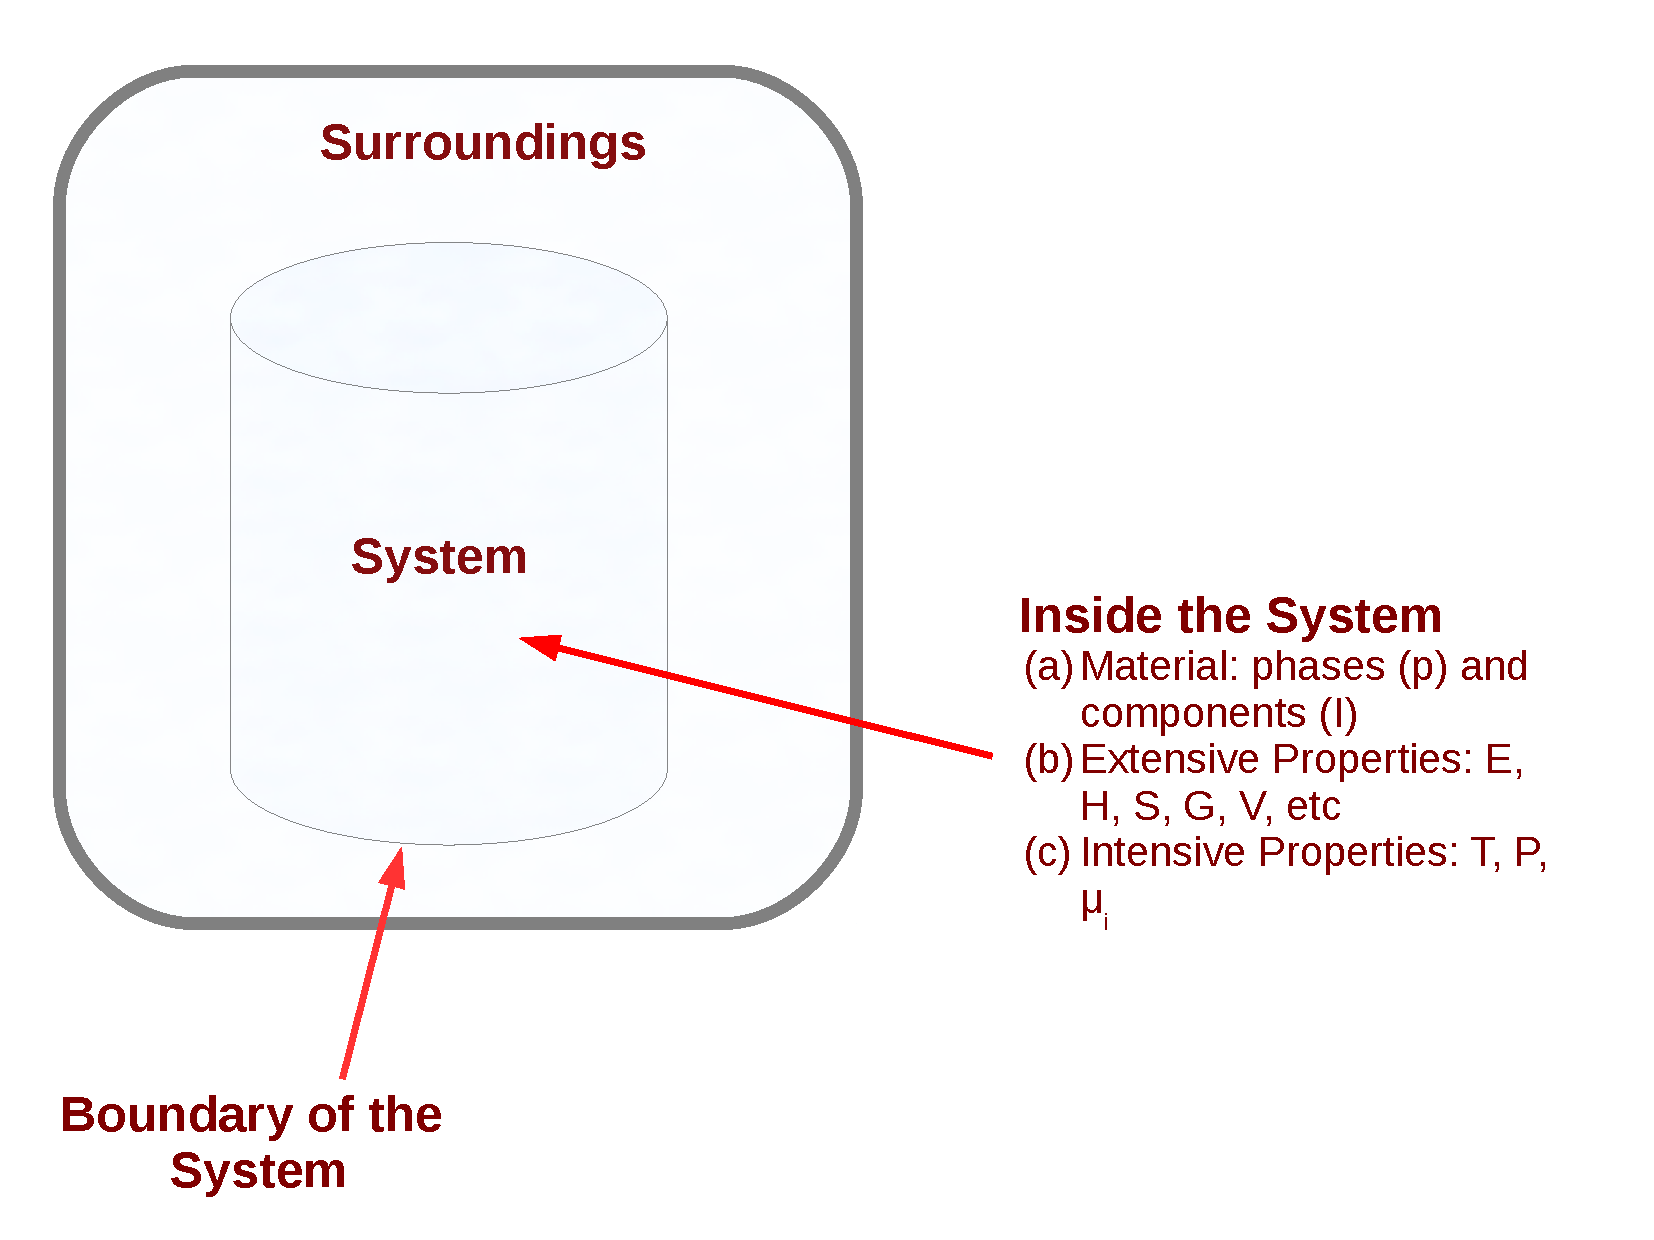
\includegraphics[width=8cm, height=8cm]{./../Pics/Fig_SystemDefinition}
       \caption{Elements of a thermodynamic problem: system and surroundings separated by well-defined borders.}\label{Chapter:Introduction:Fig:Domain}
     \end{center}
   \end{figure}
   
   
%%% Subsection
   \subsection{System, Surroundings and Boundaries}\label{Chapter:Introduction:Section:Introduction:SystemSurroundingsBoundaries}\index{System}\index{System!Boundaries}\index{System!Surroundings}
   In practice, any thermodynamic analysis starts by defining the domain of interest, which can be a volume in space or quantity of matter (Fig.~\ref{Chapter:Introduction:Fig:Domain}). This domain is called {\it system}, \ie any 3-D region of physical space with prescribed mass; the remaining of the domain is called {\it surroundings} (or {\it neighbourhood}) which is limited by {\it boundaries}. The {\it boundary} is a surface that encloses the {\it system} and separates it from the {\it surroundings}. For example, in Fig.~\ref{Chapter:Introduction:Fig:Domain2}, liquid nitrogen is contained in a cylinder with prescribed wall thickness. In this case, the interior of the vessel with N$_{2}$ is the {\it system}, whereas the cylinder wall is the border of the system. 

% Figure
   \begin{figure}[h]
     \begin{center}
       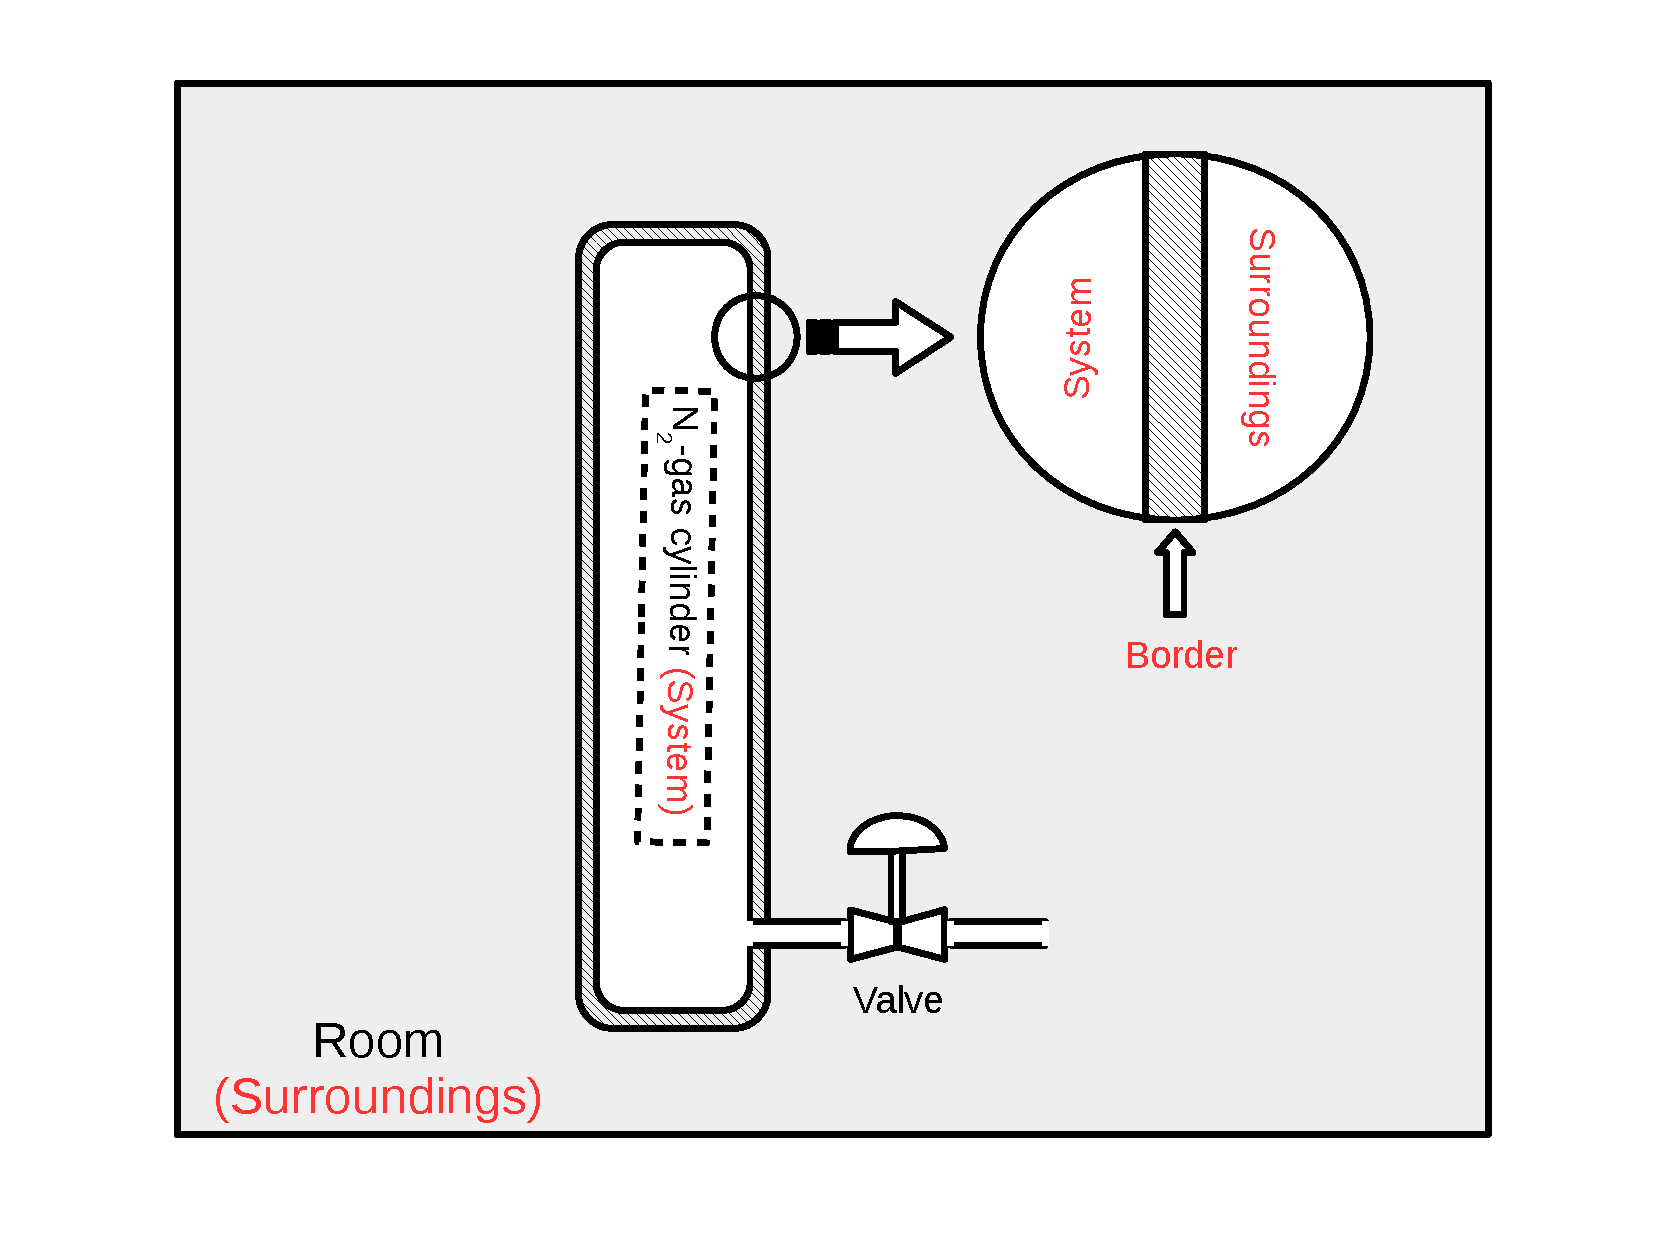
\includegraphics[width=9cm, height=7cm]{./../Pics/Fig_SystemDefinition2}
        \caption{Example of a well-defined thermodynamic problem: cylinder stored in a room. Pressurised liquid N$_{2}$ contained in a cylinder is the system, whereas the remaining of the room are the surroundings. Cylinder's wall is the border of the system.}\label{Chapter:Introduction:Fig:Domain2}
     \end{center}
   \end{figure}

   For convenience, sometimes we may want to divide the {\it system} into multiple {\it sub-systems} and analyse them individually, or to combine several small {\it systems} into larger {\it super-systems}. The choice depends on the conditions of the domain of interest and how mass and energy flow across the {\it sub-systems}. For example, in Fig.~\ref{Chapter:Introduction:Fig:Domain2}, if the valve is opened to the room (at atmospheric pressure) would be vaporised ({\it phase change}) and occupy the room. In such scenario, the room and the cylinder become the {\it system} bounded by the room's walls; the area outside the room is now the surroundings. Multiple different configurations can be drawn from this rather simple cylinder-room set.

%%% Table
   \begin{table}[h]
     \begin{center}
      \begin{tabular}{|c|c|c|}
         \hline
                      & {\bf Mass} & {\bf Energy} \\
                      & {\bf Exchange} & {\bf Exchange} \\
         \hline
         {\bf Open}   & {\it yes}  & {\it yes}    \\
         {\bf Closed} & {\it no}   & {\it yes}    \\
         {\bf Isolated}&{\it no}   & {\it no}     \\
         \hline 
      \end{tabular}  
        \caption{System and control volumes: energy and mass transfer.}\label{Chapter:Introduction:Table:System}
     \end{center}
   \end{table}
   
   If mass and energy are allowed to flow across the {\it boundaries}, we say that the {\it system} is {\bf open}, otherwise if only the energy is allowed to flow (\ie be transferred) across the {\it boundaries}, the {\it system} is assumed to be {\bf closed}. If both energy and mass can not be transferred across the {\it boundaries} the system is assumed {\bf isolated}, in such case, where there is no energy flow, the boundary is called {\bf adiabatic} (Table~\ref{Chapter:Introduction:Table:System}).\index{System!Open}\index{System!Closed}\index{System!Isolated}\index{System!Adiabatic}\index{Adiabatic}

% Figure
   \begin{figure}[h]
     \begin{center}
        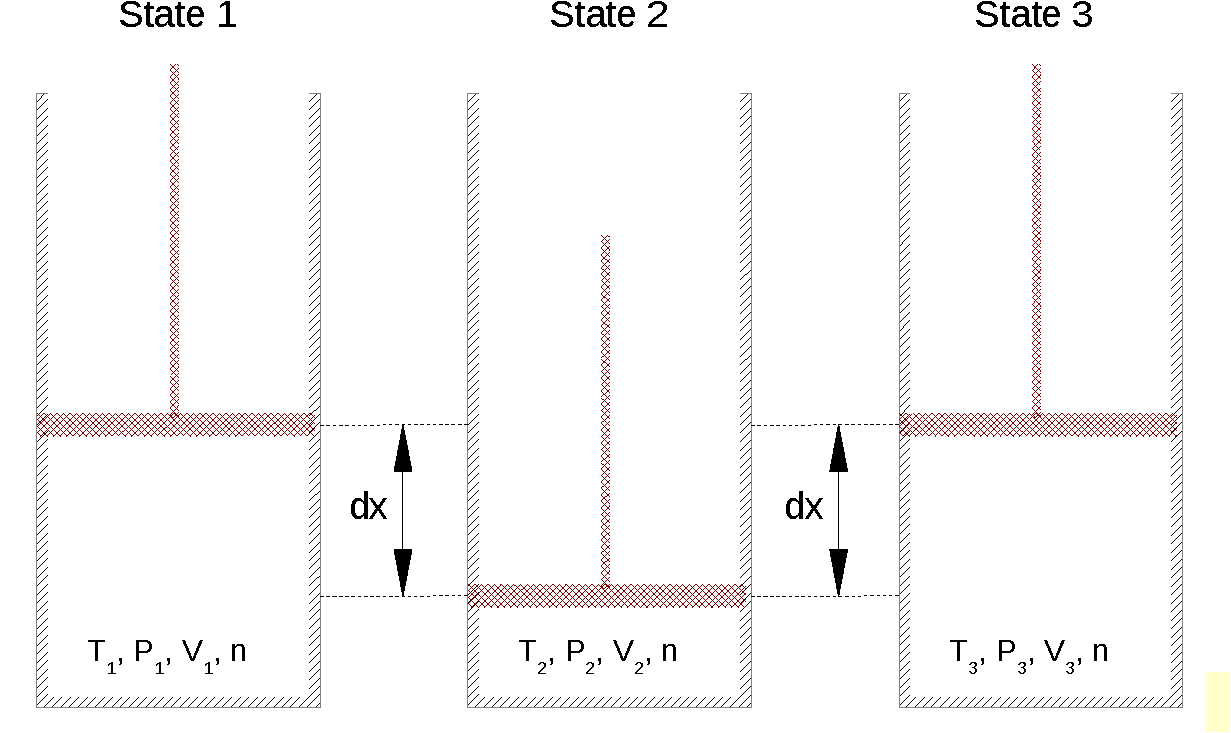
\includegraphics[width=0.7\columnwidth,clip]{./../Pics/Fig_SystemDefinition3}
        \caption{Cylinder-piston system with extensive/intensive properties.}\label{Chapter:Introduction:Fig:Domain3}
     \end{center}
   \end{figure}

   In the example depicted in Fig.~\ref{Chapter:Introduction:Fig:Domain2}, assuming an ordinary industrial liquid N$_{2}$ (at subzero temperature) cylinder, if the valve is closed, then there is no fluid flow from the cylinder to the room, but heat is flowing from the environment to the cylinder cavity. Such system is said to be {\bf closed}.
\medskip
% Example
\begin{MyExample}{\begin{center}{\bf Example}\end{center}}
\begin{example}\label{Chapter:Introduction:Example1}
  \citep{Reisel_Book} For the following systems, determine whether the system described is best modelled as an isolated, closed or open system:
  \begin{enumerate}[a)]
     \item steam flowing through a turbine\;\;$\rightarrow$\;\; {\it Open.}
     \item an incandescent light bulb\;\;$\rightarrow$\;\; {\it Closed.}
     \item an inflated tire\;\;$\rightarrow$\;\; {\it Isolated if the tire is at rest, but closed if it is in movement.}
     \item a rock formation 200 m below the surface of the earth\;\;$\rightarrow$\;\; {\it Open.}
     \item a tea kettle containing boiling water\;\;$\rightarrow$\;\; {\it Open as water steam can still leave the system.}
     \item a human body\;\;$\rightarrow$\;\;{\it Depending on the circumstances, a human body can be either open (\eg during meals, physical exercises etc) or closed.}
     \item an engine's radiator\;\;$\rightarrow$\;\; {\it Closed}.
  \end{enumerate}
\end{example}
\end{MyExample}

%%% Subsection
   \subsection{Properties and State of Substances}\label{Chapter:Introduction:Section:Introduction:ExtensiveIntensiveProperties}\index{Extensive Properties}\index{Intensive Properties}\index{System!Extensive Properties}\index{System!Intensive Properties}
   The {\it material} in a system is composed of phases (e.g., solid, liquid, gas) with distinct physical and chemical properties, thus with explicit {\it boundaries} (\ie interfaces) between phases. A quantitative property of a system (\eg temperature and pressure) describes macroscopic characteristics, which may vary with time (\ie time-dependent property). Two states of the matter are equivalent if they have the same properties, \eg in a cylinder-piston system (Fig.~\ref{Chapter:Introduction:Fig:Domain3}) containing {\it n} moles of pure gas, if {\it state 1} is defined by temperature $T_{1}$, pressure $P_{1}$ and volume $V_{1}$, and {\it state 3} is defined is by temperature $T_{3}$, pressure $P_{3}$ and volume $V_{3}$, state 1 is {\it equivalent} to state 3 {\it if and only if} $T_{1} = T_{3}$ and $P_{1} = P_{2}$. 
\medskip

   Thermodynamic properties may be classified as either {\bf extensive} or {\bf intensive}. An extensive property is a property that depends on the mass (or extent) of the substance (\ie size) in the system. Examples of extensive properties are total mass, total volume, total internal energy etc. An intensive property is a property that is independent of the mass of the substance, examples are temperature and pressure.

   Thus, for example, if a system is cut in half, its intensive properties remain unchanged, while extensive properties are cut in half. The ratio of an extensive property to the mass (\ie property per unit mass) is called {\bf specific property}, and this is an {\bf intensive} property.. The ratio of an extensive property to the number of moles of the substance in the system (\ie property per mole) is referred as {\bf molar property}, also this is an {\bf intensive} property.

   
%%%
%%% SECTION
%%%
   \section{Thermodynamic Work and Heat}\label{Chapter:Introduction:Section:ThermodynamicWorkHeat}\index{Work}\index{Heat}
   \begin{subequations}
     Work can be defined as a form of energy transfer due to changes in external macroscopic physical properties of a thermodynamic system. It can be expressed in several forms: magnetic, mechanical, electrical etc.

     For example, in a piston-cylinder system (Fig.~\ref{Chapter:Introduction:Fig:Domain3}) work is produced by the system when the gas volume expands against an external force (states 2-3). Similarly, an external force is responsible for the compression of the gas, \ie work is given to the system (states 1-2). In these cases (expansion and compression of a gas), work transfer (to or from the system) is due to the application of a finite force on the system boundary (piston).

     It is clear that the boundary (\ie volume limited by the cylinder wall and the piston-head) either contracts or expands due to external and internal forces acting on it. In other words, applied forces acting over a distance (piston length) result in mechanical energy transfer (\ie work). For an infinitesimal displacement of the piston within a cylinder, {\it dx}, the work ($W$) can be defined by
     \begin{equation}
        dW = F dx,\label{Chpt01_Work1}
     \end{equation}
     where $F$ is the force acting vertically upon the piston. If the movement occurs over a finite distance, the resulting work can be obtained by integrating Eqn.~\ref{Chpt01_Work1}. By convention, {\bf work} is assumed {\bf positive} if the displacement is in the same direction as the force applied, and {\bf negative} when the force and the displacement are in opposite directions. Thus, from stage 2 to 3 (Fig.~\ref{Chapter:Introduction:Fig:Domain3}), the force is acting upon the piston with contraction of the volume of the gas $\left(V^{t}\right)$,
     \begin{displaymath}
       dW = -PAd\left(\frc{V^{t}}{A}\right),
     \end{displaymath}
     where $A$ is the area of the piston (constant), then
     \begin{shaded}
        \begin{equation}
           dW = -PdV^{t}.\label{Chpt01_Work2}
        \end{equation}
     \end{shaded}
     Equation~\ref{Chpt01_Work2} describes the work undertaken by any process when volume changes due to transfer of energy from or to the system. If the fluid undertakes a compression (thus reduction of volume) due pressure over the system, the work is positive, otherwise when the system produces work (\ie transfer energy to the surroundings through expansion of the boundaries), the work is considered as negative.

     \citet{Devoe_Book} defined {\bf heat} as `the transfer of energy across the boundary caused by a temperature gradient at the boundary'. This concept will naturally lead to the {\it First Law of Thermodynamics} (Section~\ref{Chapter:LawsOfThermodynamics:FirstLaw}).     

   \end{subequations}
   
%%%
%%% SECTION
%%%
   \section{Thermodynamic Equilibrium and the Zeroth Law}\label{Chapter:Introduction:Section:Equilibrium_ZerothLaw}\index{Equilibrium!Mechanical}\index{Equilibrium!Chemical}\index{Equilibrium!Thermal }\index{Laws of Thermodynamics!Zeroth law}
   During thermodynamic processes, the state of the system may change due to gradients of different variables within or across boundaries, \ie
   \begin{enumerate}[a)]
        \item pressure gradients result in momentum transfer and/or convective mass transport;
        \item temperature gradients produce heat exchange, and;
        \item concentration gradients yields to diffusive mass transfer.
   \end{enumerate}
   Changes in the state of the system will continue until all internal or cross-boundary gradients vanish. When all gradients are non-existent the system exhibits no further changes and at such conditions, the system is said to be in {\bf thermodynamic equilibrium}.\index{Equilibrium!Thermodynamic}
      A system is in {\bf thermodynamic equilibrium} if it satisfies the criteria for mechanical, thermal and chemical equilibrium.  
% Figure
   \begin{figure}[h]
     \begin{center}
        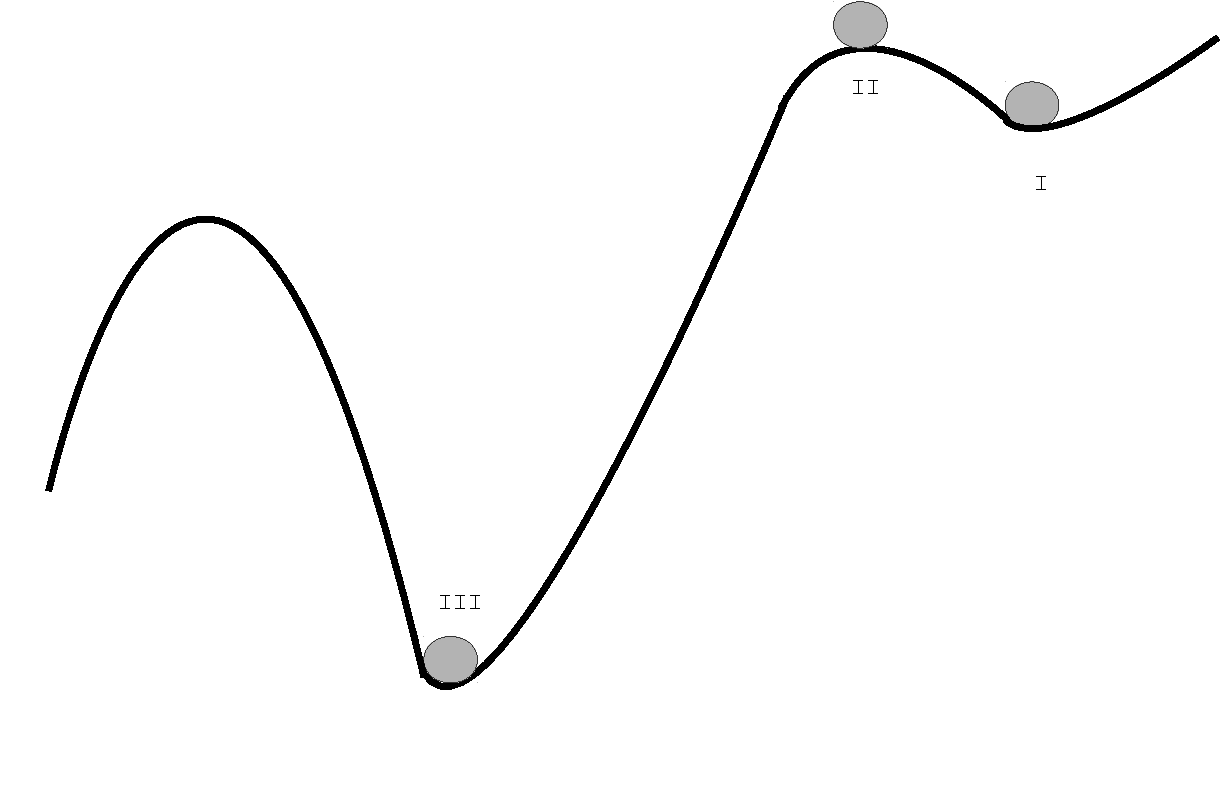
\includegraphics[width=0.7\columnwidth,clip]{./../Pics/Fig_SystemDefinition4}
        \caption{Potential energy variation in a particle motion.}\label{Chapter:Introduction:Fig:Domain4}
     \end{center}
   \end{figure}

\medskip

   Let's consider a particle initially at rest (state I in Fig.~\ref{Chapter:Introduction:Fig:Domain4}). The total energy associated with this particle is the sum of potential and kinetic energies (assuming that the particle is inert and is kept at a constant temperature). If the particle is perturbed by a mechanical force of very small magnitude, it will eventually return to its initial state (\ie at a finite time), however if the perturbation is sufficiently large the particle is unlikely to return to the original state. In this scenario, the particle is said to be in a {\it unstable equilibrium}\index{Equilibrium!Mechanical!Unstable}. Now, let's assume that the particle is at state II, where any perturbation can move it to either state I or III. In such conditions, the particle is said to be in a {\it meta-stable equilibrium}\index{Equilibrium!Mechanical!Meta-stable}. Finally, if the particle is at state III, it will remain at this condition even under the influence of large perturbation. At such conditions, the particle is said to be in a {\it stable equilibrium}\index{Equilibrium!Mechanical!Stable}. If $E_{p}$ is the potential energy of the particle and $x$ is the displacement in the vertical direction, the equilibrium states can be described as
   \begin{equation}
      \begin{cases}
         \text{Stable equilibrium (III):}  & \frc{\partial E_{p}}{\partial x} = 0 \text{ and } \frc{\partial^{2} E_{p}}{\partial x^{2}} > 0; \\
          \\
         \text{Unstable equilibrium (II):}  & \frc{\partial E_{p}}{\partial x} = 0 \text{ and } \frc{\partial^{2} E_{p}}{\partial x^{2}} < 0; \\
          \\
         \text{Meta-stable equilibrium (I):}  & \frc{\partial E_{p}}{\partial x} = 0 \text{ and } \frc{\partial^{2} E_{p}}{\partial x^{2}} = 0; \\
      \end{cases}
   \end{equation}
   These mechanical equilibrium states can be extended to thermodynamic systems during phase changes, where the potential energy and the spatial coordinate are replaced by the {\it Gibbs free energy} and intensive/extensive properties, respectively.

   \bigskip

   The concept of thermal equilibrium is intuitively simple: if two or more bodies at distinct temperatures are in physical contact, the bodies will tend to a single temperature at a finite time. This principle is called the {\bf Zeroth Law} of thermodynamics and was first stated by J. C. Maxwell in 1872:
   \begin{MyBlock}{\bf Zeroth Law of Thermodynamics} 
     ``Bodies whose temperatures are equal to that of the same body have themselves equal temperatures.”
   \end{MyBlock}
   This definition enables the use of thermometers as devices to measure the temperature of bodies. Traditional thermometers have two components, a bulb containing mercury and a linear temperature scale. The mercury bulb is maintained at a relatively low temperature $\left(\text{\ie } T_{\text{th}}\le 35^{\circ}\text{C}\right)$, whereas a body is at temperature $T>T_{\text{th}}$. When the thermometer and the body are in contact, from the {\it zeroth law}, both will reach the same temperature $T$ at a finite time. The temperature difference triggers a volumetric expansion of the mercury that can be readily observed in the scaled glass column.

\begin{FinalSummaryBlock}{Summary}
    In this chapter, some fundamental concepts of thermodynamic properties were revised and the their relationships with energy were introduced. Heat and work, two of the most important forms of energy exchange studied in thermodynamics, were introduced. The Zeroth law of thermodynamics was introduced and its application to temperature measurement was briefly explored.

    Most of these fundamentals concepts are familiar to you through other engineering courses. However, the remaining of this document strongly relies on this concepts and ideas, and you should understand all these concepts before moving forward.
\end{FinalSummaryBlock}

\begin{problem}\label{pr:pb1}
  A simple problem environment
BLELBLEBLE
\end{problem}

   
\begin{comment}
%%%
%%% SECTION
%%%
\section{Laws of Thermodynamics}\label{Chapter:Introduction:Section:LawsThermodynamics}\index{Laws of Thermodynamics}

%%%
%%% SECTION
%%%
\section{Zeroth Law}\label{zeroth_law}\index{Laws of Thermodynamics!Zeroth law}



%%%
%%% SECTION
%%%
\section{First Law}\label{Chapter:LawsOfThermodynamics:FirstLaw}\index{Laws of Thermodynamics!First law}


%%%
%%% SECTION
%%%
\section{Second Law}\label{second_law}\index{Laws of Thermodynamics!Second law}




blablabla \cite{batchelor_1967} \cite{SmithVanNess_Book}
\index{Reynolds Transport theorem}

\begin{exmp}
This is the example.
\end{exmp}

%%%
%%% SECTION 1
%%%
\section{Module 01: Introduction and Principles}\label{Section:01}

%%% SUBSECTION
\subsection{A Few Important Definitions}
  
   \begin{enumerate}[i)]
%
       \item The thermodynamic system is the part of the universe we are considering. We are free to choose boundary conditions that best represent the problem.
%
       \item \red{System} is defined as a quantity of matter or a region in space chosen for study. The mass or region outside the system is called the {\it surroundings};
%
       \item Real or imaginary surfaces that separate the system from its surroundings is called the {\it boundary};
%
      \item Systems may be considered to be {\it closed} or {\it open}, depending on whether a fixed mass or a fixed volume in space is chosen for study; 
%
      \item A closed system (also known as a {\it control mass}) consists of a fixed amount of mass, and no mass can cross its boundary. However, energy (in the form of heat or work) may cross the boundary -- and the volume of a closed system does not have to be fixed; 
%
      \item When neither energy nor mass is allowed to cross the boundary, that system is called an {\it isolated system};
%
      \item An open system (or {\it control volume}) is a properly selected region in space. It usually encloses a device that involves mass flow such as a compressor, turbine, or nozzle.
%
      \item The {\it material} in a system is composed of phases (e.g., solid, liquid, gas) with distinct physical and chemical properties;
%
      \item The {\it composition} of each phase is described by a series of discrete chemical formula units (i.e., chemical components) -- e.g., water/steam $\left(\right.$H$_{2}$O$\left.\right)$, ammonia $\left(\right.$NH$_{3}\left.\right)$, carbon dioxide $\left(\right.$CO$_{2}\left.\right)$, etc;
%
      \item {\it Properties} are macroscopic quantities associated with the system and may be defined experimentally (\eg P, V, T etc). These quantities are either intensive or extensive, \ie either independent or linearly dependent on the amount of matter.
%
      \item {\it State functions} are function of any thermodynamic property, and as such they can be either extensive or intensive (\eg internal energy, enthalpy, entropy, Gibbs free energy, Helmholtz free energy etc).
%
      \item In an arbitrary thermodynamic transformation where $Q$ is the net amount of heat absorbed by the system, and $W$ is the net amount of work done on the system, the 1$^{\text{st}}$ Law states that
          \begin{displaymath}
             \Delta U = Q + W,
          \end{displaymath}
where $U$ is the internal energy.
%
      \item In thermally isolated system (\ie contained within adiabatic walls):
          \begin{displaymath}
             Q = 0 \Longrightarrow \Delta U = W. 
          \end{displaymath}
%
      \item For mechanically isolated system,
          \begin{displaymath}
             W = 0 \Longrightarrow \Delta U = Q.
          \end{displaymath}
%
      \item The 1$^{\text{st}}$ Law is a statement of energy conservation and defines $U$ as an extensive state function. In an infinitesimal transformation, the first law can be expressed in differential form as,
          \begin{displaymath}
             dU = \delta Q + \delta W.
          \end{displaymath}
This expression states that d$U$ is a total (\ie exact) differential for an infinitesimal transformation. $Q$ and $W$ are process-dependent and are not state functions, therefore $\delta Q$ and $\delta W$ are approximations (\ie not exact). 
%
      \item In thermodynamic cycles, changes in the system may lead to a number of equilibrium and non-equilibrium states, but ending in exactly the same state as the start. By definition, all state variables (\eg $U$) are unchanged in a cycle thus,
          \begin{displaymath}
             \displaystyle\oint\limits_{C} d U = 0,
          \end{displaymath}
around any closed cycle $C$, or
          \begin{displaymath}
             \displaystyle\oint\limits_{C} \delta Q + \displaystyle\oint\limits_{C} \delta W = 0.
          \end{displaymath}
Although in general $\displaystyle\oint\limits_{C} \delta Q\ne 0$ and $\displaystyle\oint\limits_{C} \delta W\ne 0$, these line integrals depend on the closed path $C$.
%
      \item For a process to be {\it reversible} two conditions must be satisfied: (a) it must be quasistatic, and (b) there must be no friction. A quasistatic process is a successive set of equilibrium states of the system. It is an idealisation as it is required to be carried out infinitely slowly. As reversible processes are infinitely slow, it is always essentially in equilibrium.
%
      \item In {\it irreversible} processes, variables and state functions continuously change through a number of non-equilibrium states until reaching equilibrium.
%
      \item If the PVT behaviour of a fluid is represented by $PV^{n}=$ constant, then
           \begin{itemize}
              \item If $n = 0\;\;\Longrightarrow P =$ constant, and the process is {\it isobaric}; 
              \item If $n = 1\;\;\Longrightarrow PV =$ constant, and the fluid is an {\it ideal gas};
              \item If $n = \infty\;\;\Longrightarrow$ the process is {\it isochoric} (\ie constant volume);
              \item If $n = \gamma=\frc{C_{p}}{C_{v}}\;\;\Longrightarrow$ the process is {\it adiabatic} (\ie isentropic).
           \end{itemize}
%
   \end{enumerate}

%%% SUBSECTION
\subsection{A Few Important Derivations}
  
   \begin{enumerate}[i)]
%
      \item Derive \blue{$C_{p}-C_{v}=R$}:

           From the statement of the First Law $dU = dQ + dW$ with $dU=C_{v}dT$ and $dW = -PdV$,
              \begin{equation}
                  \red{dQ = C_{v}dT + PdV},\label{Mod01_1Law_1}
              \end{equation}
           where $V$ is the molar volume. For constant external pressure,
              \begin{displaymath}
                  C_{p}dT = dQ = C_{v}dT + PdV,
              \end{displaymath}
           And assuming \underline{ideal gas}, the equation of state, $PV=RT$, can be differentiated,
              \begin{displaymath}
                  dT = d\left(\frc{P V}{R}\right) \Longrightarrow dT =\frc{P}{R}dV + \frc{V}{R}\cancelto{=0\text{ (constant pressure)}}{dP}  \Longrightarrow PdV = RdT
              \end{displaymath}
           Now, replacing in the previous equation,
              \begin{eqnarray}
                  C_{p}dT &=& C_{v}dT + PdV \nonumber \\
                  C_{p}dT &=& C_{v}dT + RdT \;\;\;\blue{\left(\times \frc{1}{dT}\right)} \nonumber\\
                  C_{p} &=& C_{v} + R \Longrightarrow \red{C_{p}-C_{v}=R}  \label{Mod01_1Law_CpCv}
              \end{eqnarray}
%
      \item Derive \blue{$dQ=C_{p}dT-\frc{RT}{P}dP$}: 

           Again from $dU = dQ + dW$,
           \begin{displaymath}
               dQ = dU -dW = dU + PdV = C_{v}dT + PdV,
           \end{displaymath}
           however as $C_{p}+C_{v}=R$,
           \begin{eqnarray}
               dQ &=& \left(C_{p}-R\right)dT + PdV \nonumber \\
                  &=& C_{p}dT - RdT + PdV. \nonumber
           \end{eqnarray}
           Differentiating the ideal gas equation of state,
           \begin{eqnarray}
               PV &=& RT \;\;\text{ (differentiating both sides)} \nonumber \\
               d(PV) &=& d(RT) \nonumber \\
               PdV + VdP &=& RdT \nonumber
           \end{eqnarray}
           Replacing $RdT$ in the relation above for $dQ$,
           \begin{eqnarray}
               \red{dQ} &=& C_{p}dT - RdT + PdV. \nonumber \\
                  &=& C_{p}dT - PdV - VdP + PdV \nonumber \\
                  &=& C_{p}dT - VdP \red{= C_{p}dT - \frc{RT}{P}dP} \label{Mod01_1Law_2}
           \end{eqnarray}
%
      \item Derive \blue{$dQ=\frc{C_{p}}{R} PdV + \frc{C_{v}}{R} VdP$}:

           Again from $dU = dQ + dW$,
           \begin{displaymath}
               dQ = dU -dW = dU + PdV = C_{v}dT + PdV,
           \end{displaymath}
           Differentiating the ideal gas equation of state, $T=\frc{PV}{R}$
           \begin{displaymath}
                dT = \frc{P}{R}dV + \frc{V}{R}dP.
           \end{displaymath}
           Replacing it in the previous relation, and with $C_{p}-C_{v}=R$,
           \begin{eqnarray}
             \red{dQ} &=& C_{v}\frc{P}{R}dV + C_{v}\frc{V}{R}dP + PdV = \left(\frc{C_{v}}{R}+1\right)PdV + \frc{C_{v}}{R}VdP \nonumber \\
                &=& \left(\frc{C_{p}-R}{R}+1\right)PdV + \frc{C_{v}}{R}dP \nonumber \\
                      &=&  \red{\frc{C_{p}}{R} PdV + \frc{C_{v}}{R} VdP } \label{Mod01_1Law_3}
           \end{eqnarray}
%
      \item We just derived 3 fundamental relations based on the 1$^{\text{st}}$ Law -- Eqns.~\ref{Mod01_1Law_1},~\ref{Mod01_1Law_2} and ~\ref{Mod01_1Law_3}.
%
      \item Isentropic/Polytropic Relations: in adiabatic processes, no heat exchange is allowed between the system and the surroundings ($dQ=0$). For mechanically reversible adiabatic (\ie isentropic) \blue{compression / expansion} of ideal gasses (Eqn.~\ref{Mod01_1Law_1}),
           \begin{eqnarray}
             dQ &=& C_{v}dT + PdV =0 \nonumber \\
             dT &=& -\frc{P}{C_{v}}dV  \;\; \left(\text{Constraint: } C_{v}\ne 0\right) \nonumber \\
             dT &=& -\frc{RT}{V C_{v}}dV \;\; \Rightarrow \;\; \frc{dT}{T} = - \frc{R}{C_{v}}\frc{dV}{V}. \label{Mod01_1Law_4}
           \end{eqnarray}
           Integrating Eqn.~\ref{Mod01_1Law_4} and assuming $C_{v}$ is constant,
           \begin{eqnarray}
              \int\limits_{T_{1}}^{T_{2}} \frc{dT}{T} &=& \frc{R}{C_{v}}\int\limits_{V_{1}}^{V_{2}}\frc{dV}{V} \nonumber \\
              \left.\ln{T}\right|_{T_{1}}^{T_{2}} &=& \left.-\frc{R}{C_{v}}\ln{V}\right|_{V_{1}}^{V_{2}} \nonumber \\
              \ln{\frc{T_{2}}{T_{1}}} &=& -\frc{R}{C_{v}}\ln{\frc{V_{2}}{V_{1}}} = \ln{\left(\frc{V_{1}}{V_{2}}\right)^{\frac{R}{C_{v}}}} \nonumber \\
              \frc{T_{2}}{T_{1}} &=& \left(\frc{V_{1}}{V_{2}}\right)^{\frac{R}{C_{v}}} \nonumber
           \end{eqnarray}

           Now, defining the heat capacity ratio (or isentropic index), $\gamma\equiv\frc{C_{p}}{C_{v}}$, and using the relation $C_{p}-C_{v}=R$,
           \begin{equation}
              \gamma = \frc{C_{p}}{C_{v}} = \frc{C_{v}+R}{C_{v}} = 1 + \frc{R}{C_{v}},\label{Mod01_Gamma}
           \end{equation}
           the relation above becomes
           \begin{equation}
              \red{TV^{\gamma-1} = \text{ constant}}\label{Mod01_1Law_5}
           \end{equation}

           Now, from Eqn.~\ref{Mod01_1Law_2} and assuming $C_{p}$ is constant and different from zero,
           \begin{eqnarray}
             dQ &=& C_{p}dT - \frc{RT}{P} = 0 \nonumber \\
             \int\limits_{T_{1}}^{T_{2}}\frc{dT}{T} &=& \frc{R}{C_{p}}\int\limits_{P_{1}}^{P_{2}}\frc{dP}{P} \nonumber \\
             \left.\ln{T}\right|_{T_{1}}^{T_{2}} &=& \left.\frc{R}{C_{p}} \ln{P}\right|_{P_{1}}^{P_{2}} \nonumber \\
             \ln{\frc{T_{2}}{T_{1}}} &=& \ln{\left(\frc{P_{2}}{P_{1}}\right)^{\frac{R}{C_{p}}}} \nonumber \\
             \frc{T_{2}}{T_{1}} &=& \left(\frc{P_{2}}{P_{1}}\right)^{\frac{R}{C_{p}}}.\nonumber
           \end{eqnarray}
            Using the $\gamma$ relation, Eqn.~\ref{Mod01_Gamma},
           \begin{equation}
              \red{TP^{\frac{1-\gamma}{\gamma}} = \text{ constant}}\label{Mod01_1Law_6}
           \end{equation}

           Finally, from Eqn.~\ref{Mod01_1Law_3},
           \begin{eqnarray}
             dQ &=& \frc{C_{v}}{R}VdP + \frc{C_{p}}{R}PdV = 0 \nonumber \\
              \frc{C_{v}}{\cancel{R}}VdP = -\frc{C_{p}}{\cancel{R}}PdV &\Longrightarrow& C_{v}\int\limits_{P_{1}}^{P_{2}} \frc{dP}{P} = -C_{p}\int\limits_{V_{1}}^{V_{2}}\frc{dV}{V} \nonumber \\
              \left.\ln{P}\right|_{P_{1}}^{P_{2}} &=& -\left.\frc{C_{p}}{C_{v}}\ln{V}\right|_{V_{1}}^{V_{2}} \nonumber \\
              \frc{P_{2}}{P_{1}} &=& \left(\frc{V_{1}}{V_{2}}\right)^{\frac{C_{p}}{C_{v}}} \nonumber
           \end{eqnarray}
            Using the $\gamma$ relation, Eqn.~\ref{Mod01_Gamma},
           \begin{equation}
              \red{PV^{\gamma} = \text{ constant}}\label{Mod01_1Law_7}
           \end{equation}
%
      \item {\bf Relation for Entropy Changes:} From the First Law equation,
           \begin{equation}
              dU = dQ - PdV,\label{Mod01_1Law_Eqn}
           \end{equation} 
           If we differentiate the enthalpy equation -- $H = U + PV$.
                \begin{displaymath}
                    dH = dU + d(PV) = dU + PdV +VdP,
                \end{displaymath}
           and replace in Eqn.~\ref{Mod01_1Law_Eqn}:
                \begin{displaymath}
                    dH - \cancel{PdV} - VdP = dQ - \cancel{PdV} \;\;\Rightarrow \;\; dQ = dH - VdP
                \end{displaymath}
           For ideal gas, $C_{p}=\left(\frac{dH}{dT}\right)_{P}$ and $V=\frc{RT}{P}$,
                \begin{eqnarray}
                  dQ &=& C_{p}dT - \frc{RT}{P}dP\;\;\;\;\;\times\left(\frc{1}{T}\right) \nonumber \\
                  \frc{dQ}{T} &=& \frc{C_{p}}{T}dT - \frc{R}{P}dP \nonumber \\
                  dS &=& \frc{C_{p}}{T}dT - \frc{R}{P}dP, \nonumber
                \end{eqnarray}
           where $S$ is the molar entropy of ideal gas. Integrating from state 0 to state 1,
                \begin{eqnarray}
                    \int\limits_{S_{0}}^{S_{1}} dS &=& \int\limits_{T_{0}}^{T_{1}} \frc{C_{p}}{T}dT - R\int\limits_{P_{0}}^{P_{1}}\frc{dP}{P} \nonumber \\
                    \left(S_{1}-S_{0}\right) &=& \int\limits_{T_{0}}^{T_{1}} \frc{C_{p}}{T}dT - R\ln{\frc{P_{1}}{P_{0}}} \;\;\;\;\times\left(\frc{1}{R}\right) \nonumber \\
                    \red{\frc{\Delta S}{R}} &=& \red{\int\limits_{T_{0}}^{T_{1}} \frc{C_{p}}{R}\frc{dT}{T} - \ln{\frc{P_{1}}{P_{0}}} }.
                \end{eqnarray}
           Although this equation was derived for mechanically reversible processes, it focuses on \underline{properties only} and is independent of the process. Thus it can be used to calculate of {\it ideal gasses}.

               
%
   \end{enumerate}

%%% SUBSECTION
\subsection{General Remarks for the Course}

\begin{enumerate}[(i)]
%
   \item Do always use \blue{SI units} for calculations:
       \begin{itemize}
          \item second ($s$), meter ($m$), gram ($g$), Kelvin ($K$), mole ({\it mol});
       \end{itemize}
%
   \item Or those based on them:
       \begin{itemize}
          \item Newton ($N=kg.m.s^{-2}$), Joule ($J=N.m=kg.m^{2}.s^{-2}$), Pascal ($Pa=N.m^{-2}=kg.m^{-1}.s^{-2}$).
       \end{itemize}
%
   \item And the appropriated prefix:
      \begin{center}
        \begin{tabular}{c c c | c c c}
             \hline
             {\it Multiple} & {\it Prefix} & {\it Symbol} & {\it Multiple} & {\it Prefix} & {\it Symbol} \\
             \hline
             10$^{-15}$      & femto        & f            &   10$^{2}$     &  hecto       & h            \\
             10$^{-12}$      & pico         & p            &   10$^{3}$     &  kilo        & k            \\
             10$^{-9}$       & nano         & n            &   10$^{6}$     &  mega        & M            \\
             10$^{-6}$       & micro        & $\mu$        &   10$^{9}$     &  giga        & G            \\
             10$^{-3}$       & milli        & m            &   10$^{12}$    &  tera        & T            \\
             10$^{-2}$       & centi        & c            &   10$^{15}$    &  peta        & P            \\
             \hline
        \end{tabular}
      \end{center}
%
   \item Most of the time, we need to convert units during our calculations. Thus if we want to convert pressure ($P$) from {\it atm} to {\it psi} (pounds per square inch):
      \begin{displaymath}
        P = 5\;\cancel{\text{atm}} \times \textcolor{red}{\displaystyle\frac{14.70\;\text{psi}}{1\;\cancel{\text{atm}}}} = 73.50\;psi
      \end{displaymath}
%
   \item Or, in a more complex example:
      \begin{eqnarray}
        h_{7} &=& h_{6} + v_{6}\left(P_{7}-P_{6}\right) \nonumber \\
              &=& 706.9\textcolor{red}{\frac{kJ}{kg}} + 1.1111\times 10^{-3}\textcolor{blue}{\frac{m^{3}}{kg}}\left(210.0-7.4\right)\textcolor{blue}{bar} \nonumber \\
              &=& 706.9\textcolor{red}{\frac{kJ}{kg}} + 1.1111\times 10^{-3}\textcolor{blue}{\frac{\cancel{m^{3}}}{\cancel{kg}}} 202.6\;\textcolor{blue}{\cancel{bar}} \textcolor{red}{\frac{10^{5}\;\frac{\cancel{kg}}{\cancel{m}.\cancel{s^{2}}}}{1\; \cancel{bar}}} \textcolor{red}{\frac{10^{-3}\; \frac{kJ}{kg}}{1\;\frac{\cancel{m^{2}}}{\cancel{s^{2}}}}} \nonumber \\
              &=& 729.41\textcolor{red}{\frac{kJ}{kg}} \nonumber 
      \end{eqnarray} 
%
\end{enumerate}


\clearpage

%%% SUBSECTION
\subsection{Examples}

\begin{enumerate}[1)]
%%%
%%% EXAMPLE 
%%%
   \item\label{Mod01Ex01} If $P_{1}$ = 3.00 atm, $V_{1}$ = 500 cm$^{3}$, $P_{2}$ = 1.00 atm and $V_{2}$ = 2000 cm$^{3}$. Calculate the work, $W_{\text{rev}}$ (in $J$), for the expansion processes shown in Figs.~\ref{Mod01Fig01} (a) and (b).
      \begin{figure}[h]
         \begin{center}
           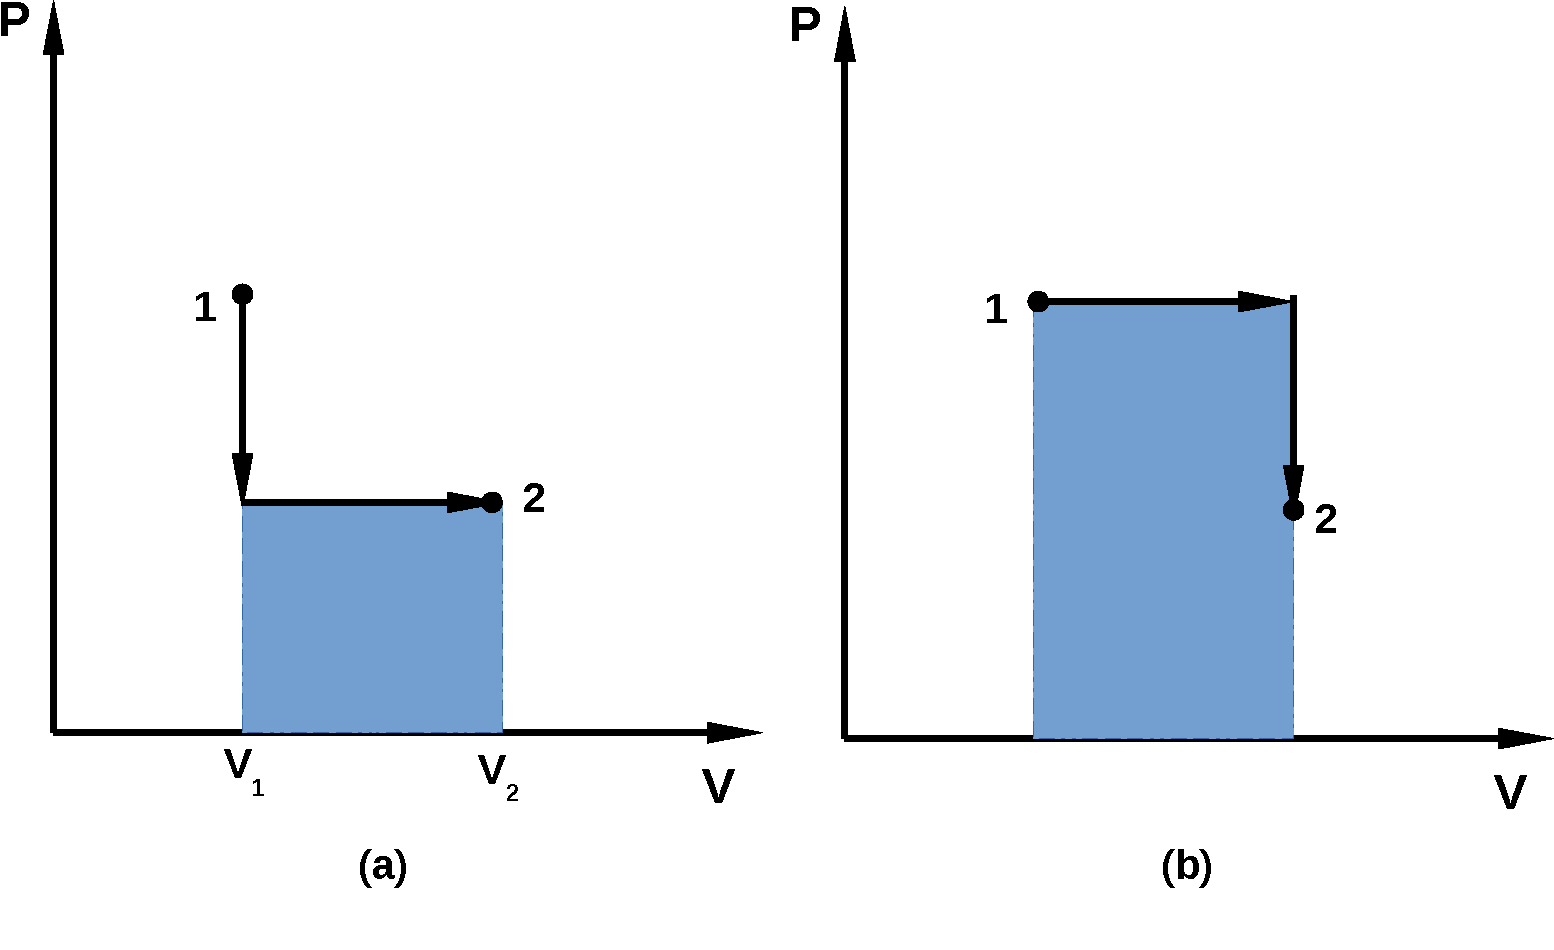
\includegraphics[width=.6\columnwidth,clip]{./Figs/Mod1Ex1}
           \vspace{-.1cm}\caption{Expansion processes (Example~\ref{Mod01Ex01}).}\label{Mod01Fig01}
         \end{center}
       \end{figure}

% SOLUTION
       \noindent{\bf Solution:} $W_{\text{rev}}$ is related to the area below the curve. Thus, we should use the $PV$ work equation:
           \begin{itemize}
              \item For process {\bf (a)}: 
                 \begin{eqnarray}
                    d W = -PdV \Longrightarrow W &=& -P_{2}\left(V_{2}-V_{1}\right) \nonumber \\
                                                 &=& - 1\text{ atm}\left(2000-500\right)\text{ cm}^{3} = -1500\text{ atm.cm}^{3} \nonumber 
                 \end{eqnarray}
                 Now we need to convert {\it atm.cm}$^{3}$ to $J$, thus using the unit conversion table:
                 \begin{eqnarray}
                     W &=& -1500\blue{\cancel{\text{ atm}}}.\red{\cancel{\text{cm}^{3}}} \frc{1.01325\times 10^{5}\blue{\cancel{\text{ Pa}}}}{1\blue{\cancel{\text{ atm}}}} \frc{1 \frc{\text{kg}}{\text{m.s}^{2}}}{1\blue{\cancel{\text{ Pa}}}} \frc{1\text{ m}^{3}}{ 100^{3} \red{\cancel{\text{ cm}^{3}}}} \nonumber \\
                       &=& -151.9875 \blue{\cancel{\frc{\text{ kg.m}^{2}}{\text{s}^{2}}}} \frc{ 1 \text{ J}}{ \blue{\cancel{\frc{\text{ kg.m}^{2}}{\text{s}^{2}}}}} \nonumber\\
                       &=& -151.9875\text{ J} \nonumber
                 \end{eqnarray}
%
              \item For process {\bf (b)}, since $P$ is constant, i.e., $P_{1}=P_{2}$:
                 \begin{eqnarray}
                    d W = -PdV \Longrightarrow W &=& -P_{1}\left(V_{2}-V_{1}\right) \nonumber \\
                                                 &=& - 3\text{ atm}\left(2000-500\right)\text{ cm}^{3} = -4500\text{ atm.cm}^{3} \nonumber \\
                                                 &=& -455.9625\text{ J} \nonumber
                 \end{eqnarray}
           \end{itemize}
\clearpage

%%%
%%% EXAMPLE
%%%
   \item Calculate the internal energy (in $J$) when 1 mol of water is isobarically heated from 25$^{\circ}$C to 30$^{\circ}$C at 1 atm. Given: densities of water are 0.9970 g.cm$^{-3}$ at 0$^{\circ}$C and 0.9956 g.cm$^{-3}$ at 100$^{\circ}$C. Molar mass and heat capacity at constant pressure of water are 18 g.mol$^{-1}$ and 1 cal.$\left(\text{g.}^{\circ}\text{C}\right)^{-1}$, respectively.

% SOLUTION
       \noindent{\bf Solution:} From the 1$^{\text{st}}$ Law, $U=Q+W$ ,and in order to calculate $U$ we first need to obtain heat ($Q$) and work ($W$). $Q$ can be obtained from the heat capacity equation
          \begin{displaymath}
             Q = m C_{p} \Delta T,
          \end{displaymath}  
          where $m$ is the mass of water can be obtained from
          \begin{displaymath}
             n = \frc{m}{MW} \Longrightarrow  m = n.MW = 1\text{ mol} . 18 \frc{\text{g}}{\text{mol}} = 18 \text{ g}
          \end{displaymath}
          $n$ and $MW$ are number of moles and molar mass, respectively. Now,
          \begin{displaymath}
             Q = m C_{p} \Delta T = 18\text{ g} . 1 \frc{\text{ cal}}{\text{g.}^{\circ}\text{C}}.\left(30-25\right)^{\circ}\text{C} = 90\text{ cal}
          \end{displaymath}  
          Now, we should calculate the work through $W=-P\Delta V$, however $V$ is not known, but we can obtain it from the density relation $V=m/\rho$, thus
          \begin{displaymath}
             W = - P\Delta V = -P\left(V_{2}-V_{1}\right) = -P\left(\frc{m}{\rho_{2}} - \frc{m}{\rho_{1}}\right) = -0.025\text{atm.cm}^{3} = -0.0006\text{ cal} 
          \end{displaymath}
          Now, calculating the internal energy,
          \begin{displaymath}
             U = Q + W = 89.9994\cancel{\text{ cal}} . \frc{ 4.186\text{ J}}{1\cancel{\text{ cal}}} = 376.7375 \text{ J}
          \end{displaymath}

\clearpage
%%%
%%% EXAMPLE
%%%
   \item A 0.3 m$^{3}$  tank contains oxygen initially at 100 kPa and 300 K. A paddle wheel within the tank is rotated until the pressure inside rise to 150 kPa. During the process 2 kJ of heat is lost to the surroundings. Determine the paddle-wheel work done (in kJ). Neglect the energy stored in the paddle wheel and assume the heat capacity at constant volume of oxygen is 0.6745 kJ.$\left(\text{kg.K}\right)^{1}$. Given molar mass of oxygen of 32 g.mol$^{-1}$.

% SOLUTION
       \noindent{\bf Solution:} The volume of the tank remains constant $V_{2}=V_{1}=V=$ 0.3 m$^{3}$ during the whole process. Thus, we can define:
            \begin{center}
              \begin{tabular}{l l l l}
                 Initial Condition & $P_{1}=$ 100 kPa   & $T_{1}=$ 300 K         & $V_{1}=$ 0.3 m$^{3}$  \\
                 Final Condition   & $P_{2}=$ 150 kPa   &                       & $V_{2}=$ 0.3 m$^{3}$ \\
                 Heat Loss         & $Q=$ -2 kJ        &                       &                    
              \end{tabular}
            \end{center}
       The compression occurs in a closed system (i.e., constant mass) and, as there is no further information, we may consider that oxygen behaves as an ideal gas. The work added to the system by the paddle can be expressed by $U=Q+W$. Our first step is to calculate $T_{2}$,
       \begin{displaymath}
          \frc{P V}{T} = \text{ constant} \Rightarrow \frc{P_{1}V_{1}}{T_{1}} = \frc{P_{2}V_{2}}{T_{2}} \Rightarrow \frc{P_{1}}{T_{1}}=\frc{P_{2}}{T_{2}} \Rightarrow T_{2} = 450\text{ K}
       \end{displaymath}
        The specific internal energy can defined by the fundamental relation, $du=C_{v}dT$ (check the units for this relation!), where $C_{v}$ is the heat capacity at constant volume thus,
       \begin{displaymath}
          \Delta U = m\Delta u = C_{v}\Delta T = Q + W,
       \end{displaymath}
       therefore, we need to obtain the mass of oxygen in the tank through the ideal gas equation of state,
       \begin{eqnarray}
         P V = n R T \Rightarrow n = \frc{m}{MW} = \frc{P V}{R T} \Rightarrow m &=& \frc{ MW P V}{R T} \nonumber \\
                                                      &=& \frc{ 32\frc{\text{ g}}{\text{mol}} 100\text{ kPa} . 0.3\text{ m}^{3}}{ 8.3143 \frc{\text{J}}{\text{mol.K}} 300\text{ K}} \nonumber \\
                                                      &=& 0.3848 \frc{\text{ g.kPa.m}^{3}}{\text{J}} \frc{1 \text{ J}}{1\text{ N.m}} \frc{1000 \text{ Pa}}{1 \text{ kPa}} \frc{ 1 \text{ N.m}^{-2}}{1\text{ Pa}} \nonumber\\
                                                      &=& 0.3848\text{ kg}\nonumber
       \end{eqnarray}
       Thus
       \begin{eqnarray}
          \Delta u = m C_{v}\Delta T = Q + W \Rightarrow W &=& m C_{v}\left(T_{2}-T_{1}\right) - Q \nonumber \\
                                                          &=& 0.3848\text{ kg} \times 0.6745 \frc{\text{kJ}}{\text{kg.K}}\times (450-300)\text{ K} - (-2 \text{ kJ}) \nonumber \\
                                                          &=& 40.9321\text{ kJ}. \nonumber
       \end{eqnarray}
       The paddle-wheel executed 40.9321 kJ of work to the system.

\clearpage
%%%
%%% EXAMPLE
%%%
   \item  Air initially occupying 1 m$^{3}$ at 1.5 bar and 20$^{\circ}$C undergoes an internally reversible compression for which $P V^{\gamma}=$ constant to a final state where the pressure is 6 bar and the temperature is 120$^{\circ}$C. Determine:
        \begin{enumerate}[(a)]
           \item Value of $\gamma$;
           \item Work and the heat transfer (in kJ).
       \end{enumerate}
       Assume that heat capacity at constant volume and molar mass of air are 0.718 kJ.$\left(\text{kg.K}\right)^{-1}$ and 29 g.mol$^{-1}$. 

% SOLUTION
       \noindent{\bf Solution:}
        \begin{center}
           \begin{tabular}{c c c c}
               {\bf State}  &   $P$ (atm)  &   $T\;\left(^{\circ}\text{C}\right)$ & $V\;\left(\text{m}^{3}\right)$ \\
                    1       &     1.5      &            20                      & 1  \\
                    2       &     6.0      &            120                     &     \\              
           \end{tabular}
        \end{center}
        \begin{enumerate}[(a)]
           \item In order to calculate the isentropic index $\gamma$, we can use any of the relations learned in the lecture,
               \begin{displaymath} 
                   P V^{\gamma} = C, \hspace{1cm} T V^{\gamma-1} = C \hspace{1cm} \text{ and/or } \hspace{1cm} T P^{\frac{1-\gamma}{\gamma}} = C.
               \end{displaymath}
               Although $P$ and $V$ is the relation initially given in the problem, we do not know the final volume of air, $V_{2}$. However, initial and final pressure and temperature are known and we can make use of this relationship to obtain $\gamma$,
               \begin{eqnarray} 
                   T P^{\frac{1-\gamma}{\gamma}} = C \Rightarrow T_{1}P_{1}^{\frac{1-\gamma}{\gamma}} = T_{2}P_{2}^{\frac{1-\gamma}{\gamma}} \nonumber \\
                   \left(\frc{P_{1}}{P_{2}}\right)^{\frac{1-\gamma}{\gamma}} = \frc{T_{2}}{T_{1}} \Rightarrow \frc{1-\gamma}{\gamma} = \frc{\ln{\frac{T_{2}}{T_{1}}}}{\ln{\frac{P_{1}}{P_{2}}}} \Longrightarrow \gamma = 1.2686  \nonumber
               \end{eqnarray}
                 
           \item Compression work can be obtained by integrating $\d W = -P dV$ from state 1 to state 2 with $P=\frac{C}{V^{\gamma}}$,
               \begin{eqnarray}
                 W_{1-2} &=& -\int\limits_{V_{1}}^{V_{2}} P dV = -\int\limits_{V_{1}}^{V_{2}}\frc{C}{V^{\gamma}} dV = -\left.\frc{C}{1-\gamma}V^{1-\gamma}\right|_{V_{1}}^{V_{2}} \nonumber \\
                         &=& -\frc{C}{1-\gamma}\left(V_{2}^{1-\gamma}-V_{1}^{1-\gamma}\right),\;\;\text{ however, as } C=P_{1}V_{1}^{\gamma}=P_{2}V_{2}^{\gamma} \nonumber \\
                         &=& -\frc{P_{2}V_{2}^{\gamma}V_{2}^{1-\gamma} - P_{1}V_{1}^{\gamma}V_{1}^{1-\gamma}}{1-\gamma} = \frc{P_{1}V_{1}-P_{2}V_{2}}{1-\gamma} \nonumber
               \end{eqnarray}
               The relation above, although important, can not be used as we do not know $V_{2}$, however we can change variables through the ideal gas relation
               \begin{eqnarray}
                  P V = n R T &\Rightarrow& n = \frc{P V}{R T } = \frc{1.5\text{ atm} \times 1\text{ m}^{3}}{ 8.3143 \frc{\text{J}}{\text{mol.K}} 293.15\text{ K}} \frc{1.01325\times 10^{5} \text{ Pa}}{1 \text{ atm}} \frc{ 1 \text{ N.m}^{-2}}{1\text{ Pa}}\frc{1 \text{ J}}{1\text{ N.m}} = 62.3580\text{ moles}\nonumber \\
                   % m &=& \frc{P_{1} V_{1} MW}{R T_{1}} = \frc{1.5\text{ atm} \times 1\text{ m}^{3} \times 29 \frac{\text{g}}{\text{mol}} } { 8.3143 \frc{\text{J}}{\text{mol.K}} 293.15\text{ K}} \frc{1 \text{ J}}{1\text{ N.m}} \frc{1.01325\times 10^{5} \text{ Pa}}{1 \text{ atm}} \frc{ 1 \text{ N.m}^{-2}}{1\text{ Pa}} = 1808.38 \text{ g}\nonumber\\
                    W &=& \frc{P_{1}V_{1}-P_{2}V_{2}}{1-\gamma} = nR\frc{T_{1}- T_{2}}{1-\gamma} \nonumber \\
                      &=& 62.3580\text{ mol} \times 8.3143 \frc{\text{J}}{\text{mol.K}} \times \frc{\left(293.15-393.15\right)\text{ K}}{1-1.2686} \nonumber \\
                      &=& 193024.2440 \text{ J} \Longrightarrow W = -193.02 \text{ kJ} \nonumber
               \end{eqnarray}
              Heat ($Q$) can be obtained from
               \begin{eqnarray}
          \Delta u &=& m C_{v}\Delta T = n MW C_{v}\Delta T = Q + W  \nonumber \\
             Q &=& n MW C_{v}\left(T_{2}-T_{1}\right) - W \nonumber \\
               &=& 62.3580\text{ mol}\times 29 \frc{\text{g}}{\text{mol}} \red{\frc{1\text{ kg}}{1000\text{ g}}}\times 0.718\frc{\text{kJ}}{\text{kg.K}}\times (393.15-293.15)\text{ K} - 193.30 \text{ kJ} \nonumber \\
                                                          &=& -63.46\text{ kJ}. \nonumber                   
               \end{eqnarray}
       \end{enumerate}


\clearpage
%%%
%%% EXAMPLE
%%%
   \item Two kg of water at 80$^{\circ}$C is mixed adiabatically with 3 kg of water at 30$^{\circ}$C in a constant pressure process of 1 atm. Find the increase in entropy $\left(\text{in kJ.K}^{-1}\right)$ of the total mass of water due to the mixing process. Assume that $C_{p}$ of water is 4.187 kJ.$\left(\text{kg.K}\right)^{-1}$. 

% SOLUTION
       \noindent{\bf Solution:} From the classic thermodynamic definition of reversible entropy processes (second law),
         \begin{displaymath}
            d S = \frc{d Q}{T}
         \end{displaymath}
         with $dQ = m C_{p}dT$, then integrating 
         \begin{eqnarray}
            \int\limits_{S_{i}}^{S_{f}} dS &=& m C_{p}\int\limits_{T_{i}}^{T_{f}}\frc{dT}{T} \nonumber \\
            \Delta S &=& S_{f}-S_{i} = m C_{p} \ln{\frc{T_{f}}{T_{i}}} \nonumber
         \end{eqnarray}
         Assuming that the system is adiabatic, we can calculate the final temperature $\left(T_{f}\right)$ from thermal energy conservation principles: 
         \begin{displaymath}
            m_{1}C_{p,1}T_{1} + m_{2}C_{p,2}T_{2} = \left(m_{1}+m_{2}\right)C_{p}T_{f} \rightarrow T_{f} = 50^{\circ}\text{C} = 323.15\text{ K}
         \end{displaymath}
         And the entropies are
         \begin{eqnarray}
             \Delta S_{1} &=& m_{1}C_{p,1}\ln{\frc{T_{f}}{T_{1}}} =  -0.7434\frc{\text{kJ}}{\text{K}} \nonumber \\
             \Delta S_{2} &=& m_{2}C_{p,2}\ln{\frc{T_{f}}{T_{2}}} =  0.8025\frc{\text{kJ}}{\text{K}} \nonumber 
         \end{eqnarray}
         Thus the increase in entropy of the total mass is
         \begin{displaymath}
              \Delta S_{\text{mix}} = \Delta S_{1} + \Delta S_{2} = 0.0591\frc{\text{kJ}}{\text{K}}
         \end{displaymath}
%
\end{enumerate}
\end{comment}


%%%
%%%  BIBLIOGRAPHY
%%%
%\bibliography{refbib}
 % Introduction and Review of Thermodynamics

\part{Thermodynamic Properties of Fluids}
% Aberdeen style guide should be followed when using this
% layout. Their template powerpoint slide is used to extract the
% Aberdeen color and logo but is otherwise ignored (it has little or
% no formatting in it anyway).
%
% http://www.abdn.ac.uk/documents/style-guide.pdf

%%%%%%%%%%%%%%%%%%%% Document Class Settings %%%%%%%%%%%%%%%%%%%%%%%%%
% Pick if you want slides, or draft slides (no animations)
%%%%%%%%%%%%%%%%%%%%%%%%%%%%%%%%%%%%%%%%%%%%%%%%%%%%%%%%%%%%%%%%%%%%%%
%Normal document mode%
\documentclass[10pt,compress]{beamer}
%Draft or handout mode
%\documentclass[10pt,compress,handout]{beamer}
%\documentclass[10pt,compress,handout,ignorenonframetext]{beamer}

%%%%%%%%%%%%%%%%%%%% General Document settings %%%%%%%%%%%%%%%%%%%%%%%
% These settings must be set for each presentation
%%%%%%%%%%%%%%%%%%%%%%%%%%%%%%%%%%%%%%%%%%%%%%%%%%%%%%%%%%%%%%%%%%%%%%
\newcommand{\shortname}{jefferson.gomes@abdn.ac.uk}
\newcommand{\fullname}{Dr Jeff Gomes}
\institute{School of Engineering}
\newcommand{\emailaddress}{}%jefferson.gomes@abdn.ac.uk}
\newcommand{\logoimage}{../../FigBanner/UoAHorizBanner}
\title{Chemical Thermodynamics (EX3029)}
\subtitle{Module 2: Volumetric Properties of Pure Fluids}
\date[ ]{ }

%%%%%%%%%%%%%%%%%%%% Template settings %%%%%%%%%%%%%%%%%%%%%%%%%%%%%%%
% You shouldn't have to change below this line, unless you want to.
%%%%%%%%%%%%%%%%%%%%%%%%%%%%%%%%%%%%%%%%%%%%%%%%%%%%%%%%%%%%%%%%%%%%%%
\usecolortheme{whale}
\useoutertheme{infolines}

% Use the fading effect for items that are covered on the current
% slide.
\beamertemplatetransparentcovered

% We abuse the author command to place all of the slide information on
% the title page.
\author[\shortname]{%
  \fullname\\\ttfamily{\emailaddress}
}


%At the start of every section, put a slide indicating the contents of the current section.
\AtBeginSection[] {
  \begin{frame}
    \frametitle{Section Outline}
    \tableofcontents[currentsection]
  \end{frame}
}

% Allow the inclusion of movies into the Presentation! At present,
% only the Okular program is capable of playing the movies *IN* the
% presentation.
\usepackage{multimedia}
\usepackage{animate}

%% Handsout -- comment out the lines below to create handstout with 4 slides in a page with space for comments
\usepackage{handoutWithNotes}
%\pgfpagesuselayout{2 on 1 with notes}[a4paper,border shrink=10mm]
%%%%% Color settings
\usepackage{color}
%% The background color for code listings (i.e. example programs)
\definecolor{lbcolor}{rgb}{0.9,0.9,0.9}%
\definecolor{UoARed}{rgb}{0.64706, 0.0, 0.12941}
\definecolor{UoALight}{rgb}{0.85, 0.85, 0.85}
\definecolor{UoALighter}{rgb}{0.92, 0.92, 0.92}
\setbeamercolor{structure}{fg=UoARed} % General background and higlight color
\setbeamercolor{frametitle}{bg=black} % General color
\setbeamercolor{frametitle right}{bg=black} % General color
\setbeamercolor{block body}{bg=UoALighter} % For blocks
\setbeamercolor{structure}{bg=UoALight} % For blocks
% Rounded boxes for blocks
\setbeamertemplate{blocks}[rounded]

%%%%% Font settings
% Aberdeen requires the use of Arial in slides. We can use the
% Helvetica font as its widely available like so
% \usepackage{helvet}
% \renewcommand{\familydefault}{\sfdefault}
% But beamer already uses a sans font, so we will stick with that.

% The size of the font used for the code listings.
\newcommand{\goodsize}{\fontsize{6}{7}\selectfont}

% Extra math packages, symbols and colors. If you're using Latex you
% must be using it for formatting the math!
\usepackage{amscd,amssymb} \usepackage{amsfonts}
\usepackage[mathscr]{eucal} \usepackage{mathrsfs}
\usepackage{latexsym} \usepackage{amsmath} \usepackage{bm}
\usepackage{amsthm} \usepackage{textcomp} \usepackage{eurosym}
% This package provides \cancel{a} and \cancelto{a}{b} to "cancel"
% expressions in math.
\usepackage{cancel}

\usepackage{comment} 

%% Handsout -- comment out the lines below to create handstout with 4 slides in a page with space for comments
\usepackage{handoutWithNotes}

\mode<handout>
{
\usepackage{pgf,pgfpages}

\pgfpagesdeclarelayout{2 on 1 boxed with notes}
{
\edef\pgfpageoptionheight{\the\paperheight} 
\edef\pgfpageoptionwidth{\the\paperwidth}
\edef\pgfpageoptionborder{0pt}
}
{
\setkeys{pgfpagesuselayoutoption}{landscape}
\pgfpagesphysicalpageoptions
    {%
        logical pages=4,%
        physical height=\pgfpageoptionheight,%
        physical width=\pgfpageoptionwidth,%
        last logical shipout=2%
    } 
\pgfpageslogicalpageoptions{1}
    {%
    border code=\pgfsetlinewidth{1pt}\pgfstroke,%
    scale=1,
    center=\pgfpoint{.25\pgfphysicalwidth}{.75\pgfphysicalheight}%
    }%
\pgfpageslogicalpageoptions{2}
    {%
    border code=\pgfsetlinewidth{1pt}\pgfstroke,%
    scale=1,
    center=\pgfpoint{.25\pgfphysicalwidth}{.25\pgfphysicalheight}%
    }%
\pgfpageslogicalpageoptions{3}
    {%
    border shrink=\pgfpageoptionborder,%
    resized width=.7\pgfphysicalwidth,%
    resized height=.5\pgfphysicalheight,%
    center=\pgfpoint{.75\pgfphysicalwidth}{.29\pgfphysicalheight},%
    copy from=3
    }%
\pgfpageslogicalpageoptions{4}
    {%
    border shrink=\pgfpageoptionborder,%
    resized width=.7\pgfphysicalwidth,%
    resized height=.5\pgfphysicalheight,%
    center=\pgfpoint{.75\pgfphysicalwidth}{.79\pgfphysicalheight},%
    copy from=4
    }%

\AtBeginDocument
    {
    \newbox\notesbox
    \setbox\notesbox=\vbox
        {
            \hsize=\paperwidth
            \vskip-1in\hskip-1in\vbox
            {
                \vskip1cm
                Notes\vskip1cm
                        \hrule width\paperwidth\vskip1cm
                    \hrule width\paperwidth\vskip1cm
                        \hrule width\paperwidth\vskip1cm
                    \hrule width\paperwidth\vskip1cm
                        \hrule width\paperwidth\vskip1cm
                    \hrule width\paperwidth\vskip1cm
                    \hrule width\paperwidth\vskip1cm
                    \hrule width\paperwidth\vskip1cm
                        \hrule width\paperwidth
            }
        }
        \pgfpagesshipoutlogicalpage{3}\copy\notesbox
        \pgfpagesshipoutlogicalpage{4}\copy\notesbox
    }
}
}

%\pgfpagesuselayout{2 on 1 boxed with notes}[letterpaper,border shrink=5mm]
%\pgfpagesuselayout{2 on 1 boxed with notes}[letterpaper,border shrink=5mm]


% Get rid of font warnings as modern LaTaX installations have scalable
% fonts
\usepackage{type1cm} 

%\usepackage{enumitem} % continuous numbering throughout enumerate commands

% For exact placement of images/text on the cover page
\usepackage[absolute]{textpos}
\setlength{\TPHorizModule}{1mm}%sets the textpos unit
\setlength{\TPVertModule}{\TPHorizModule} 

% Source code formatting package
\usepackage{listings}%
\lstset{ backgroundcolor=\color{lbcolor}, tabsize=4,
  numberstyle=\tiny, rulecolor=, language=C++, basicstyle=\goodsize,
  upquote=true, aboveskip={1.5\baselineskip}, columns=fixed,
  showstringspaces=false, extendedchars=true, breaklines=false,
  prebreak = \raisebox{0ex}[0ex][0ex]{\ensuremath{\hookleftarrow}},
  frame=single, showtabs=false, showspaces=false,
  showstringspaces=false, identifierstyle=\ttfamily,
  keywordstyle=\color[rgb]{0,0,1},
  commentstyle=\color[rgb]{0.133,0.545,0.133},
  stringstyle=\color[rgb]{0.627,0.126,0.941}}

% Allows the inclusion of other PDF's into the final PDF. Great for
% attaching tutorial sheets etc.
\usepackage{pdfpages}
\setbeamercolor{background canvas}{bg=}  

% Remove foot note horizontal rules, they occupy too much space on the slide
\renewcommand{\footnoterule}{}

% Force the driver to fix the colors on PDF's which include mixed
% colorspaces and transparency.
\pdfpageattr {/Group << /S /Transparency /I true /CS /DeviceRGB>>}

% Include a graphics, reserve space for it but
% show it on the next frame.
% Parameters:
% #1 Which slide you want it on
% #2 Previous slides
% #3 Options to \includegraphics (optional)
% #4 Name of graphic
\newcommand{\reserveandshow}[4]{%
\phantom{\includegraphics<#2|handout:0>[#3]{#4}}%
\includegraphics<#1>[#3]{#4}%
}

\newcommand{\frc}{\displaystyle\frac}
\newcommand{\red}{\textcolor{red}}
\newcommand{\blue}{\textcolor{blue}}
\newcommand{\green}{\textcolor{green}}
\newcommand{\purple}{\textcolor{purple}}
 
\begin{document}

% Title page layout
\begin{frame}
  \titlepage
  \vfill%
  \begin{center}
    \includegraphics[clip,width=0.8\textwidth]{\logoimage}
  \end{center}
\end{frame}

% Table of contents
\frame{ \frametitle{Slides Outline}
  \tableofcontents
}


%%%%%%%%%%%%%%%%%%%% The Presentation Proper %%%%%%%%%%%%%%%%%%%%%%%%%
% Fill below this line with \begin{frame} commands! It's best to
% always add the fragile option incase you're going to use the
% verbatim environment.
%%%%%%%%%%%%%%%%%%%%%%%%%%%%%%%%%%%%%%%%%%%%%%%%%%%%%%%%%%%%%%%%%%%%%%


%%%
%%% SECTION
%%%
\section{General Remarks}

%%%
%%% Slides
%%%
\begin{frame}
 \frametitle{Aims and Objectives}
   \begin{enumerate}
     \item<1-> In Module 1, we learnt:
       \begin{enumerate}
         \item<1-> the laws of Thermodynamics and how they describe thermal equilibrium of species in closed and open systems.
         \item<1-> how to obtain and calculate relevant thermodynamics properties for chemical species.
         \item<1-> reversibility  of processes.
       \end{enumerate} 
     \item<2-> This Module focuses on 
         \begin{enumerate}
           \item<2-> PVT behaviour of pure chemical species in equilibrium,
           \item<2-> Equations of state commonly used in industry.
         \end{enumerate}
   \end{enumerate}

\end{frame}


%%%
%%% SECTION
%%%
\section{Bibliography}
\begin{frame}
 \frametitle{Suggested References}
  Literature relevant for this module:
  \begin{enumerate}[1.]
   \item J.M. Smith, H.C. Van Ness, M.M. Abbott, $\lq$Introduction to Chemical Engineering Thermodynamics', 6$^{th}$ Edition: Chapter 3;
   \item Y.A. Cengel, M.A. Boles, $\lq$Thermodynamics -- An Engineering Approach', 5$^{th}$ Edition: Chapter 3; 
   \item M.J. Moran, H.N. Saphiro, D.D. Boettner, M.B. Bailey, $\lq$Principles of Engineering Thermodynamics', 7$^{th}$ Edition: Chapters 3;
   \item C. Borgnakke, R.E. Sonntag, $\lq$Fundamentals of Thermodynamics', 8$^{th}$ Edition: Chapter 2.
  \end{enumerate}
\end{frame}



%%%
%%% SECTION
%%%
\section{PVT Behaviour of Pure Substances}

%%%
%%% SUBSECTION
%%%
\subsection{Phase Diagram and Gibbs Rule} 

%%%
%%% Slide
%%%
\begin{frame}
 \frametitle{PVT Behaviour of Pure Substances}
 \begin{columns}
  \begin{column}[l]{0.5\linewidth}
    \begin{enumerate}\scriptsize
    \item <1-> This surface represents the \textcolor{red}{Pressure} - \textcolor{red}{specific volume} - \textcolor{red}{Temperature} -- $PVT$, relation in a pure substance;
    \item <2-> Any given coordinate in both, the surface plot and diagrams (projections), will represent values of pressure, specific volume and temperature when the substance is at equilibrium;
    \item <3-> The \textcolor{red}{Gibbs phase rule},
       \visible<3->{\begin{equation}
          \Psi = 2 + \mathcal{C} - \mathcal{P}
       \end{equation} 
       describes the number of degrees of freedom (dof), $\Psi$ (\underline{intensive variables}, e.g., temperature, pressure), in a closed system at equilibrium as a function of the number of phases ($\mathcal{P}$ = solid, liquid and/or vapour) and components, $\mathcal{C}$ (e.g., water, CO$_{2}$, N$_{2}$, etc). }
\end{enumerate}
  \end{column}
  \begin{column}[l]{0.5\linewidth}
   \begin{figure}%
    \begin{center}
     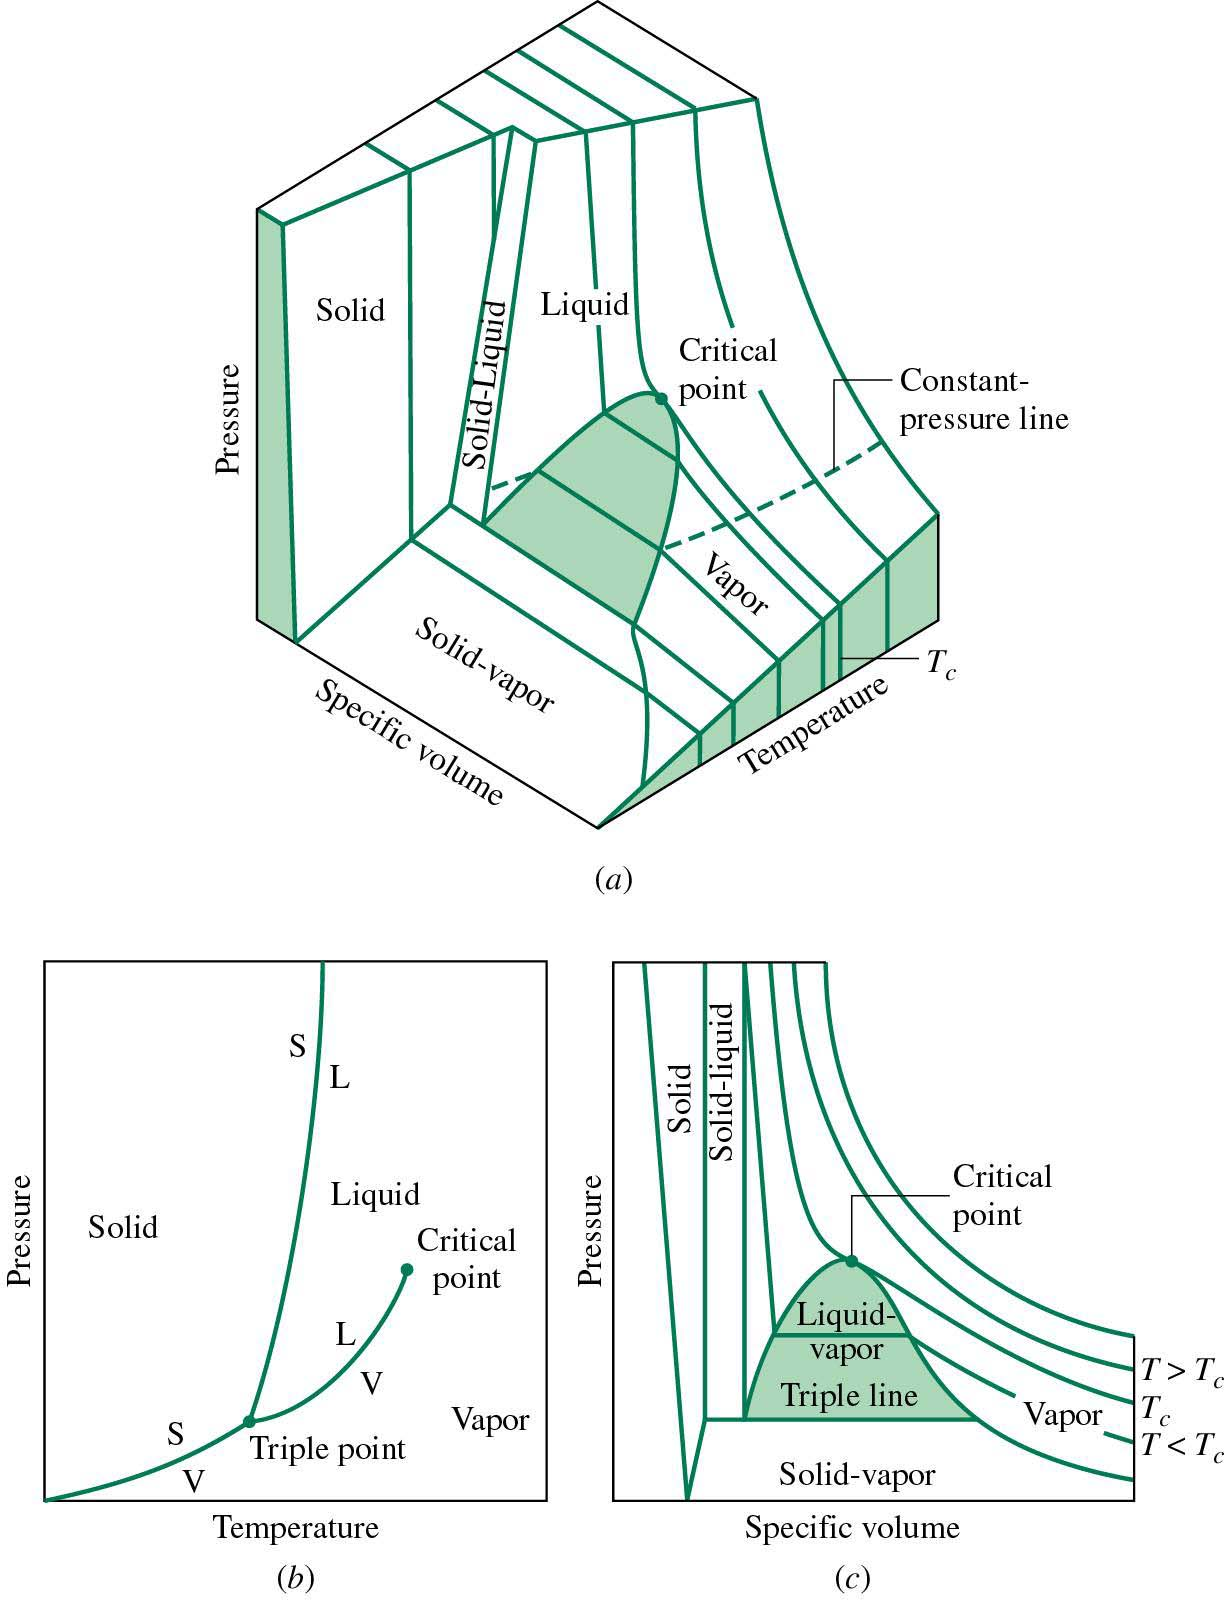
\includegraphics[width=4.cm,clip]{./../Pics/PVT_Surface.jpg}
    \end{center}
    \scriptsize\caption{\scriptsize$PVT$ volume (top) and projections onto (b) $PT$ and (c) $PV$ diagrams for a pure substance (Extracted from [4]).}
   \end{figure}    
  \end{column}
 \end{columns}
\end{frame}

%%%
%%% Slide
%%%
\begin{frame}
 \frametitle{PT Diagram}
 \begin{columns}
   \begin{column}[l]{0.5\linewidth}
     \begin{enumerate}\scriptsize
        \item<1-> The \textcolor{blue}{$PT$ phase diagram} describes fluid behaviour and phase change; 
        \item<2-> For example: \textcolor{blue}{A}-\;-\;-\textcolor{red}{B} defines a phase transition from \textcolor{blue}{liquid} to \textcolor{red}{gas} regions without crossing the phase boundary (vaporisation);
        \item <3-> {\bf Example 1:} In the $PT$ diagram for one hypothetical component -- $\textcolor{red}{\mathcal{C}=1}$, within each phase region -- $\textcolor{blue}{\mathcal{P}=1}$ (i.e., as either solid, liquid or vapour phase),
          \visible<3->{\begin{displaymath}
            \Psi = 2 + \textcolor{red}{1} - \textcolor{blue}{1} = 2
          \end{displaymath}
          \begin{enumerate}[(a)]\scriptsize
             \item  In this case, the number of degrees of freedom correspond to temperature and pressure;
             \item  Thus, within the vapour phase, temperature and pressure can readily be changed without explicit phase change or composition of the vapour phase.
          \end{enumerate}}
        \item <4-> {\bf Example 2:} However, along with the \textcolor{red}{phase-line boundary}, two phases are in equilibrium, i.e., $\textcolor{blue}{\mathcal{P}=2}$,%
          \visible<2->{\begin{displaymath}
            \Psi = 2 + \textcolor{red}{1} - \textcolor{blue}{2} = 1,
          \end{displaymath}}
     \end{enumerate}
  \end{column}
  \begin{column}[l]{0.5\linewidth}\scriptsize
          \visible<4->{when the vapour and liquid phases are in equilibrium, any change in temperature {\bf leads} to change in pressure for the system remains in equilibrium;}
      \begin{figure}%
        \begin{center}
          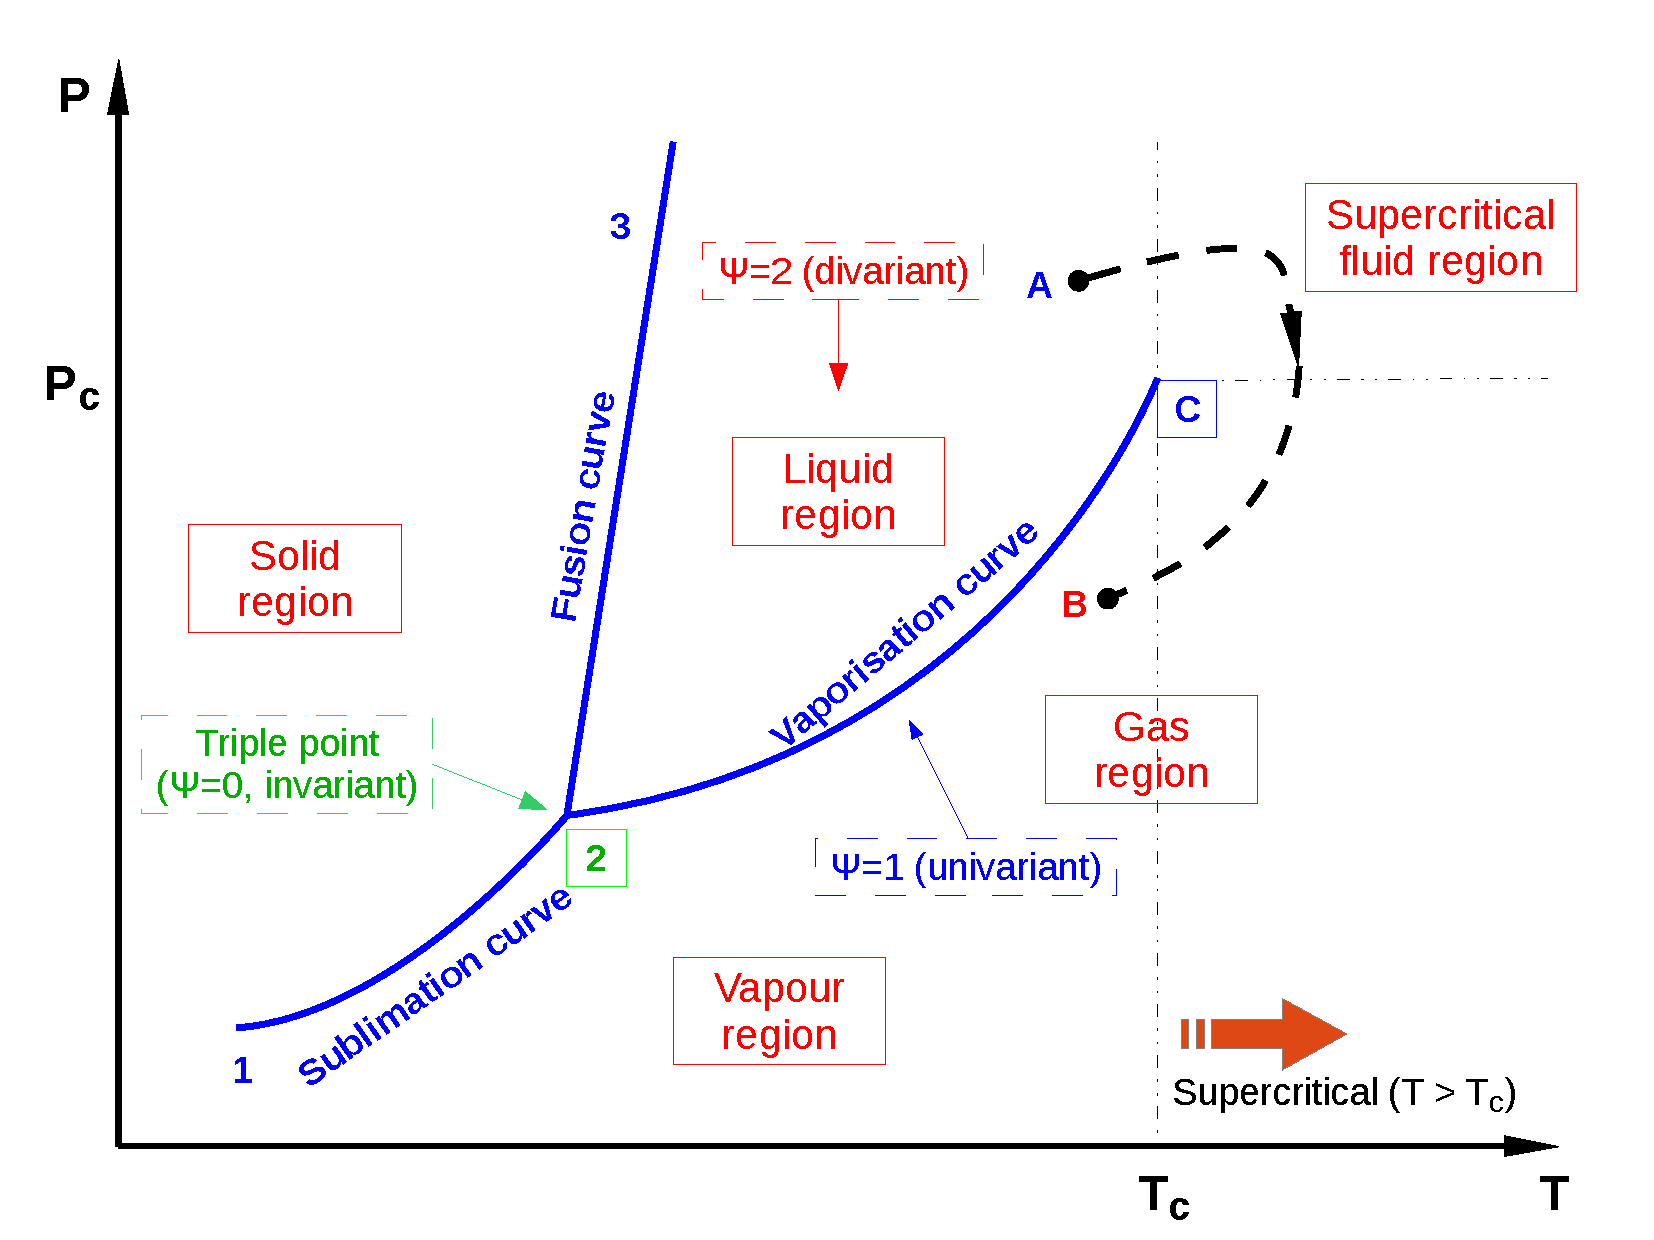
\includegraphics[width=1.05\columnwidth,clip]{./../Pics/PT_Diagram}
        \end{center}
      \end{figure}
     \begin{enumerate}\setcounter{enumi}{4}\scriptsize
        \item<5-> However, there is \red{no} information about the volume in the {\it PT} diagram.
     \end{enumerate}
  \end{column}
 \end{columns}
\end{frame}
 
%%%
%%% Slide
%%%
\scriptsize
\begin{frame}
 \frametitle{PV Diagram}
  \begin{columns}
    \begin{column}[l]{0.5\linewidth}
      \visible<1->{\begin{figure}%
        \begin{center}
          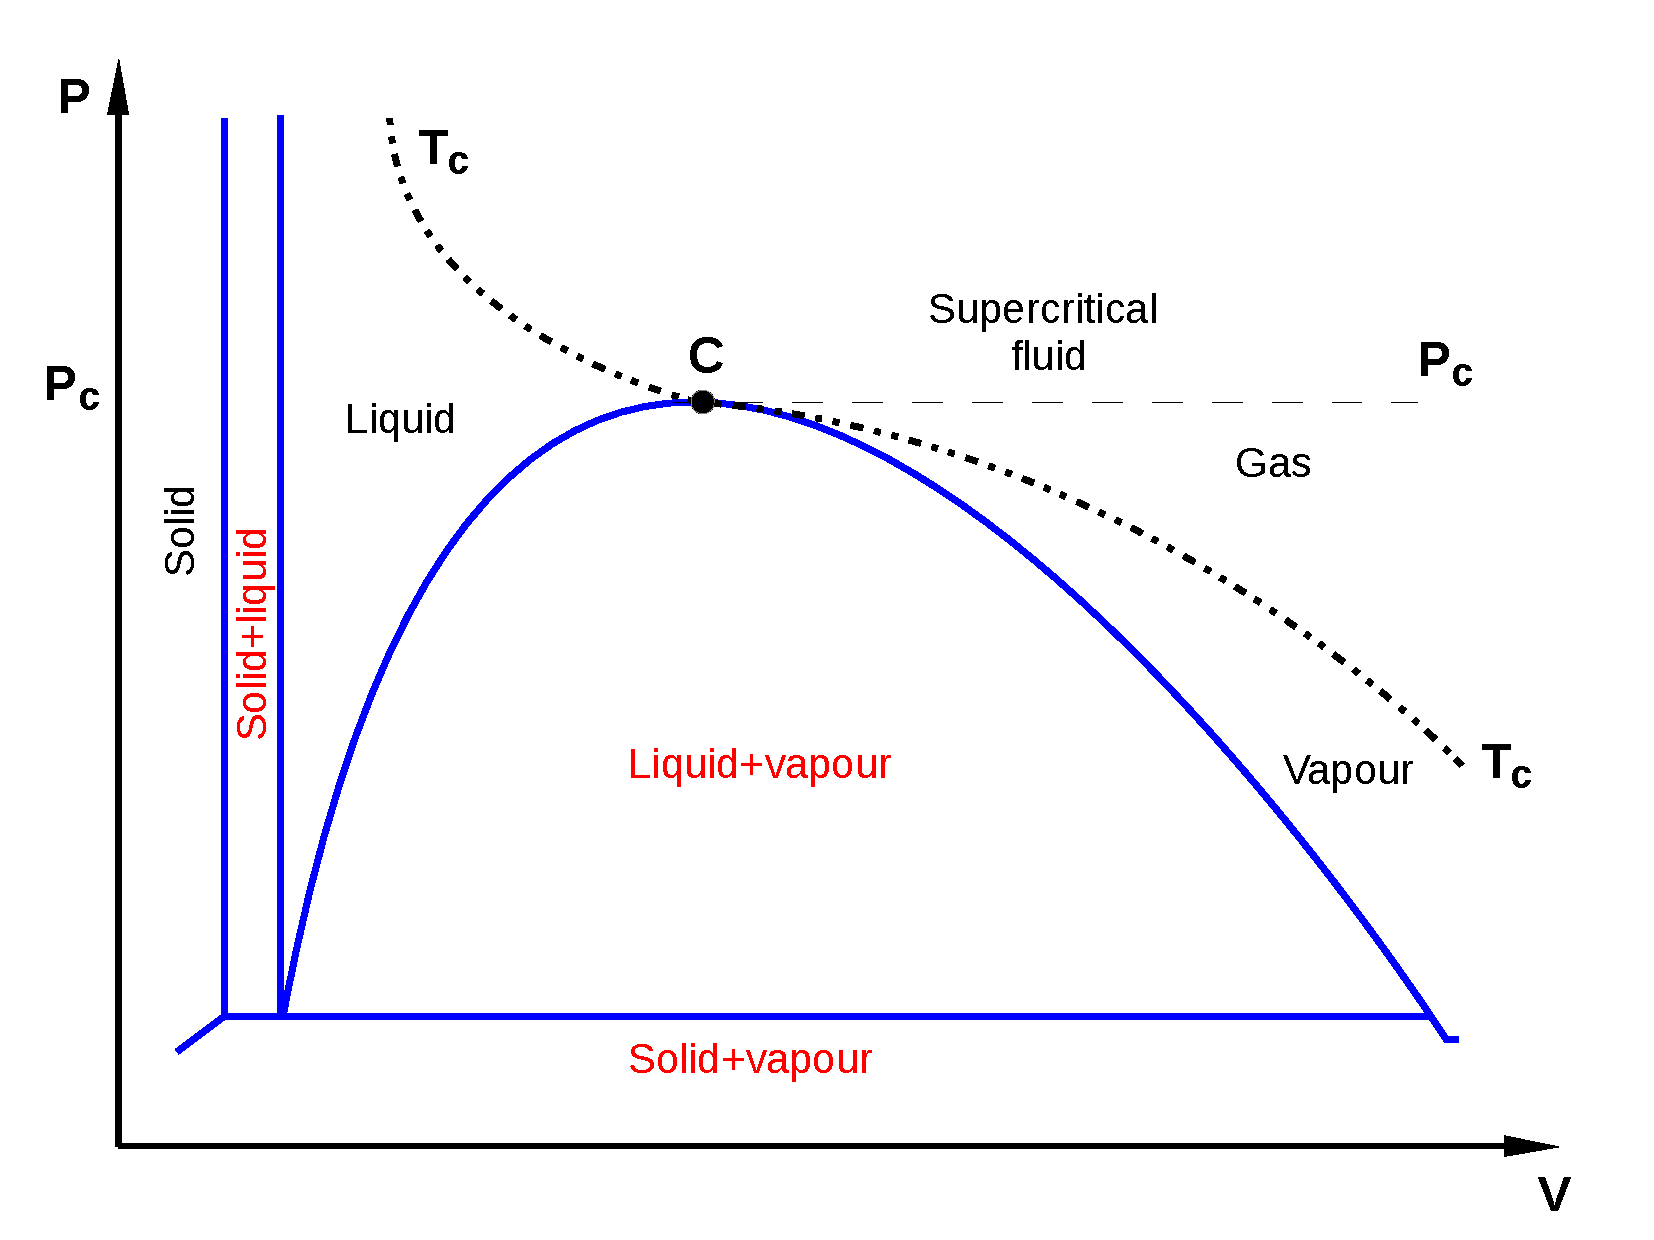
\includegraphics[width=\columnwidth,clip]{./../Pics/PV_Diagram1}
        \end{center}
      \end{figure}}
      \begin{enumerate} \scriptsize
        \item<1-> Two-phase regions (e.g., liquid+vapor) are represented by \textcolor{red}{areas} and;
        \item<2-> Lines represent the actual transition transition between \textcolor{blue}{single phase} to \textcolor{blue}{two phases} regions, thus;
        \item<2-> The \textcolor{blue}{triple point} is the horizontal line between the 3 phases;
      \end{enumerate}
    \end{column}
    \begin{column}[l]{0.5\linewidth}\scriptsize
      \visible<3->{\begin{figure}%
        \begin{center}
          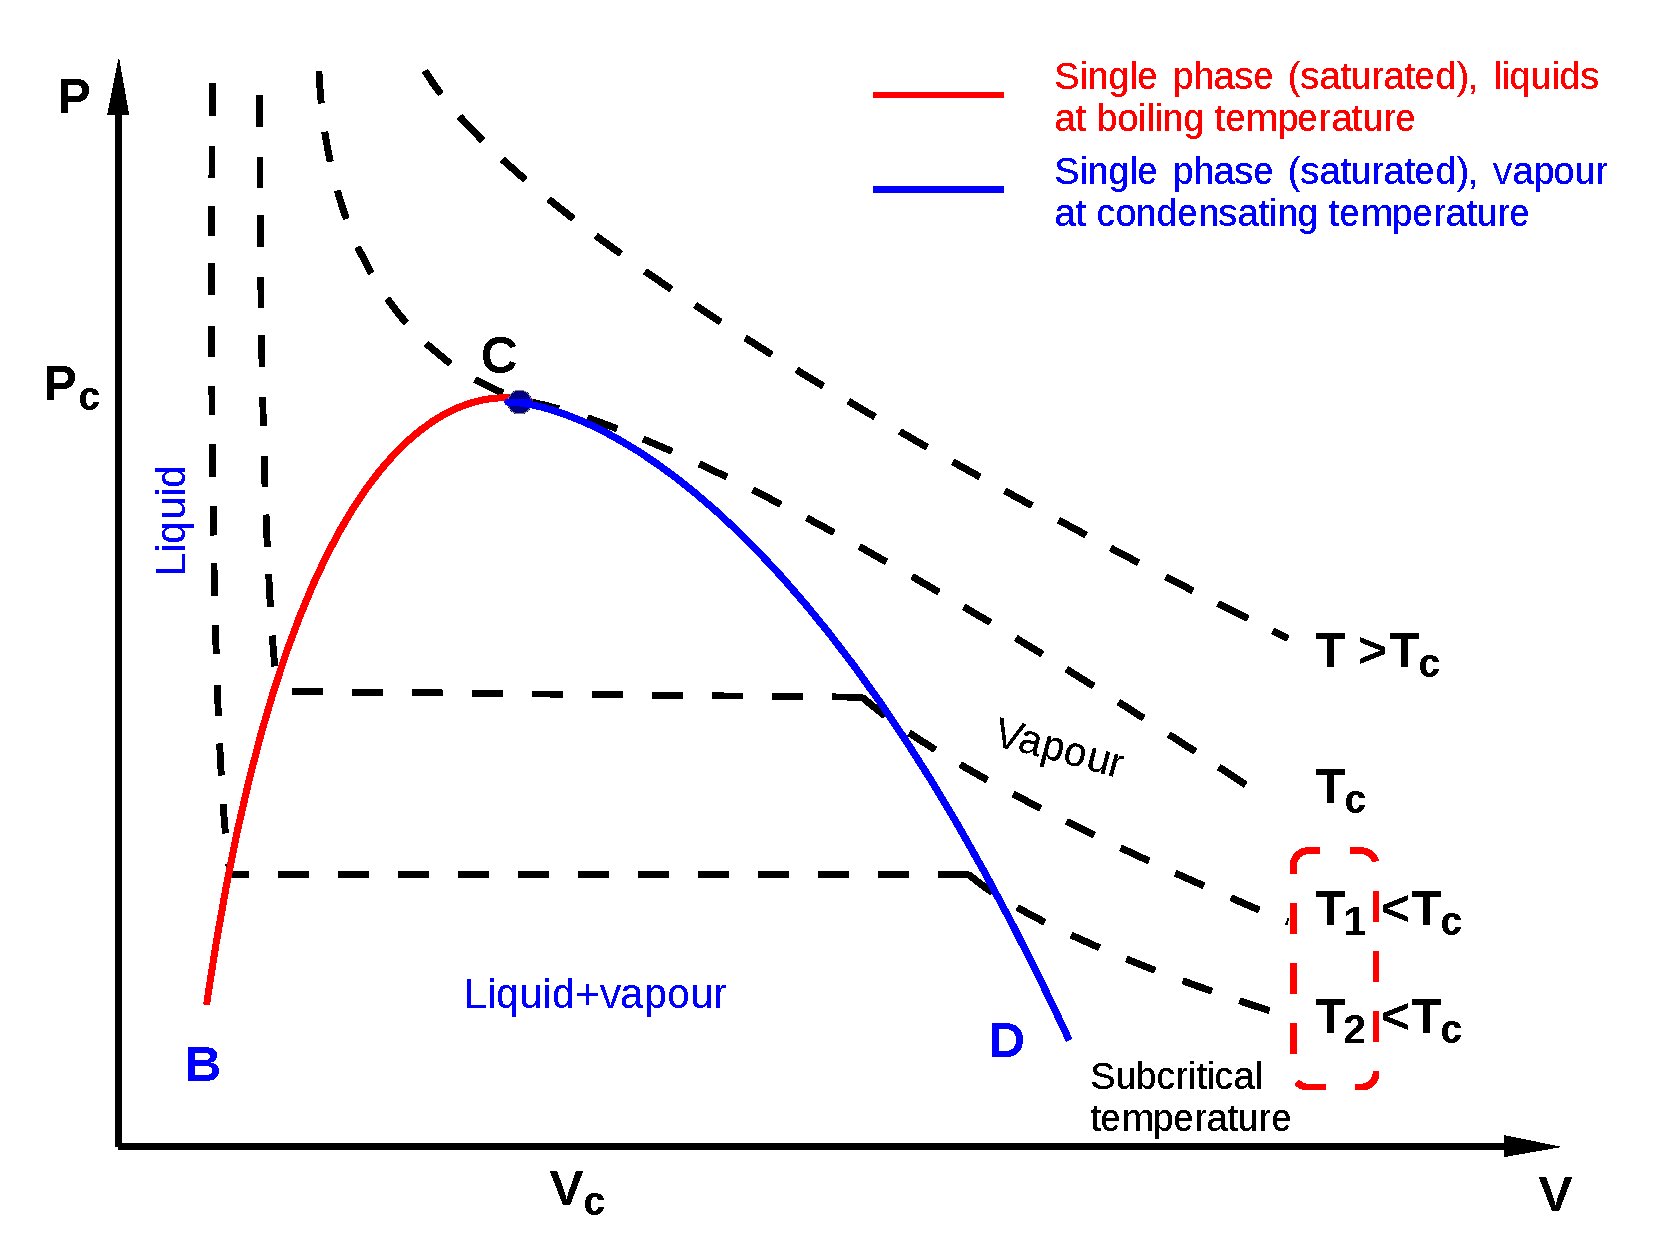
\includegraphics[width=\columnwidth,clip]{./../Pics/PV_Diagram2}
        \end{center}
      \end{figure}}
      \begin{enumerate}\setcounter{enumi}{3}
        \item<3-> The isotherms range from \textcolor{blue}{subcooled liquid} to \textcolor{blue}{superheated vapor} regions; 
        \item<3-> Isotherms are \textcolor{red}{steep} in the \textcolor{blue}{subcooled liquid}  region because liquid volumes have little changes with large change in pressure.
      \end{enumerate}
    \end{column}
  \end{columns}
\end{frame}
\normalsize

%%%% COMMENTS
\begin{comment}
%%%
%%% Slide
%%%
\scriptsize
\begin{frame}
 \frametitle{PV Diagram}
      \visible<1->{\begin{figure}%
        \begin{center}
          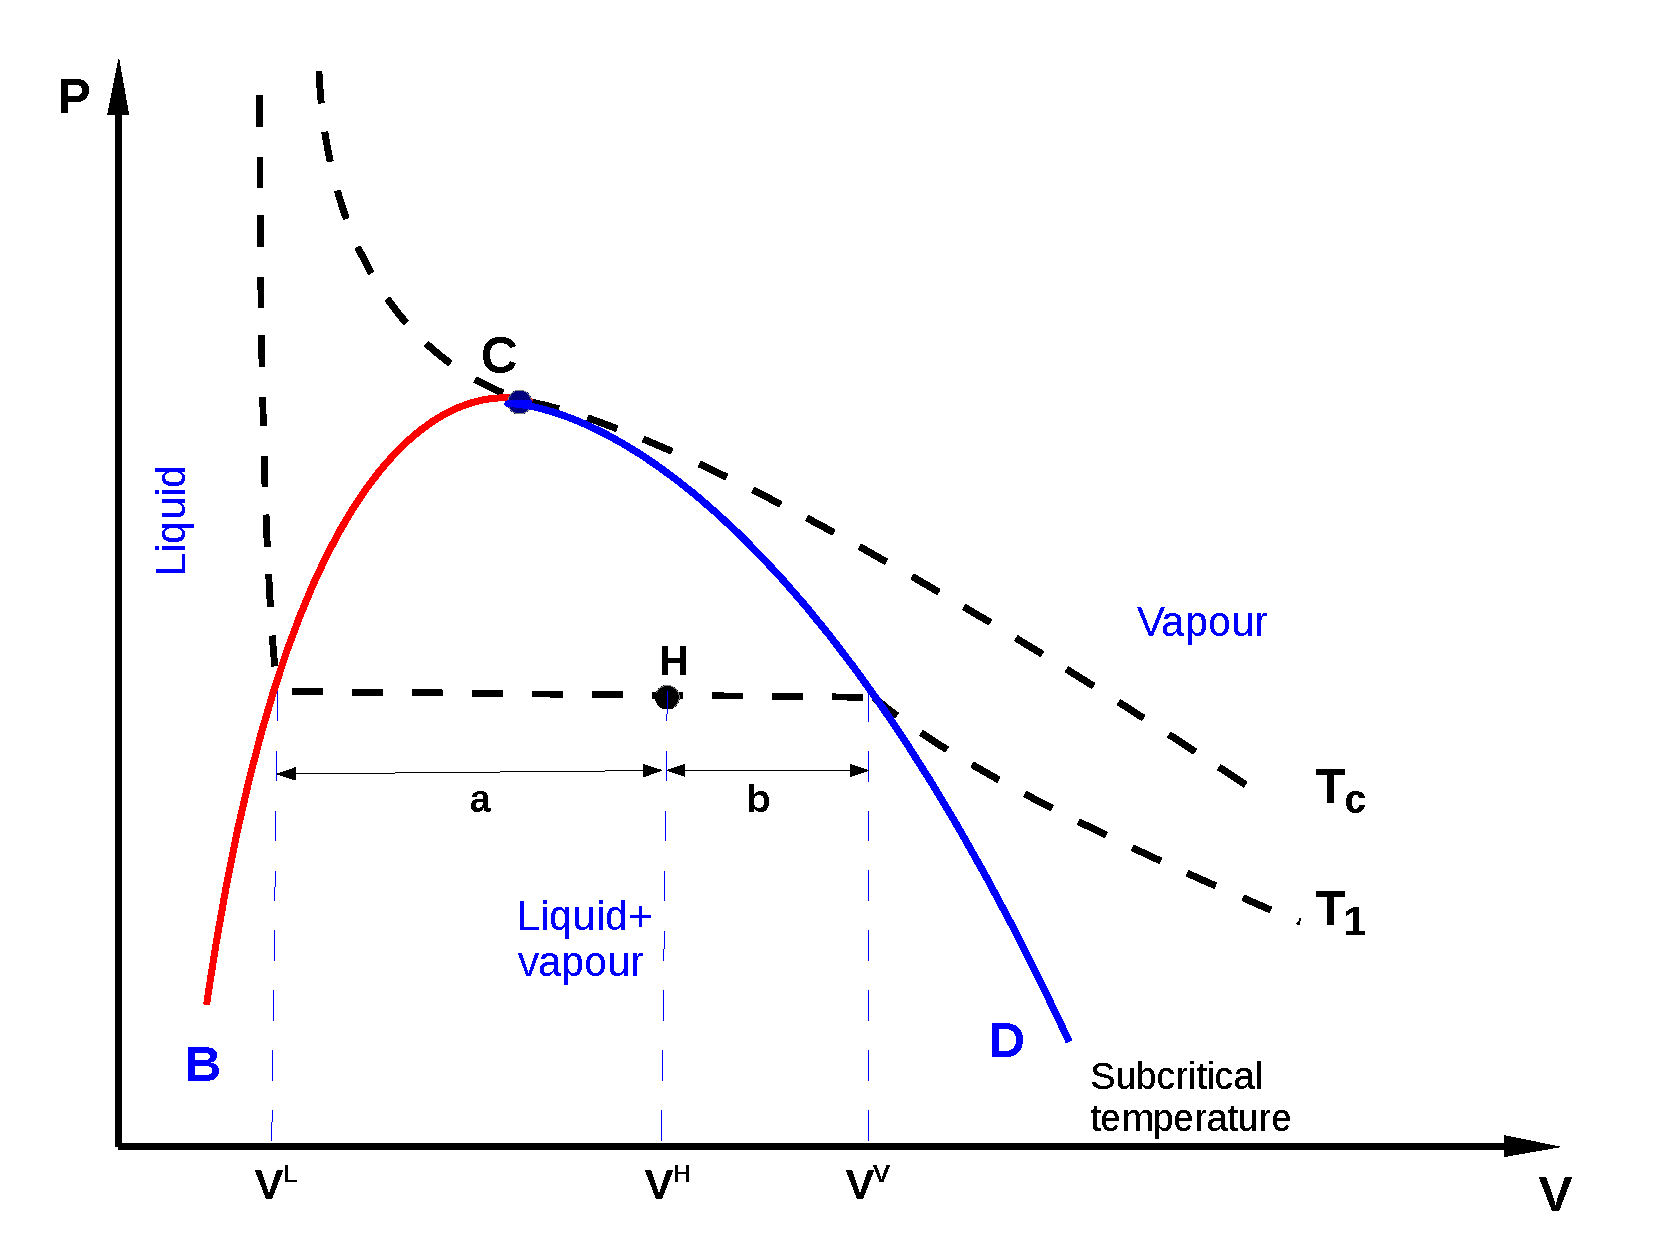
\includegraphics[width=.6\columnwidth,clip]{./../Pics/PV_Diagram3}
        \end{center}
      \end{figure}}
      \visible<2->{\begin{displaymath}
         \frc{a}{b} = \frc{V^{H}-V^{L}}{V^{V}-V^{H}} = \frc{m^{V}}{m^{L}} = \frc{\text{mass of saturated vapour}}{\text{mass of saturated liquid}}
      \end{displaymath}}
     
\end{frame}
\normalsize
\end{comment}

%%%
%%% Slide
%%%
\scriptsize
\begin{frame}
 \frametitle{Single Phase region}
    \begin{enumerate}\scriptsize
      \item<1-> \textcolor{blue}{Equations of State (EOS)} relates pressure, molar or specific volume and temperature of any \textcolor{blue}{pure homogeneous fluid} in equilibrium states;
      \item<2-> We can express it as a general functional,
          \visible<2->{\begin{displaymath}
              f\left(P, V, T\right) = 0
          \end{displaymath} 
          where $P$, $V$ or $T$ can be expressed as a function of two of this properties.}
      \item<3-> For example, we can represent the volume as $V=V\left(T,P\right)$, thus
          \visible<3->{\begin{equation}
              dV = \left(\frc{\partial V}{\partial T}\right)_{P} dT + \left(\frc{\partial V}{\partial P}\right)_{T} dP \;\;\Longrightarrow \;\; \textcolor{blue}{\frc{dV}{V} = \beta dT - \kappa dP} \label{genericV}
          \end{equation} 
            with $\beta  =  \frc{1}{V}\left(\frc{\partial V}{\partial T}\right)_{P}$ (coefficient of thermal expansion or volume expansivity coefficient) and $\kappa = -\frc{1}{V}\left(\frc{\partial V}{\partial P}\right)_{T}$ (coefficient of isothermal compressibility).
           }
      \item<4-> A few useful remarks:
        \begin{itemize}\scriptsize
          \item<4-> For \textcolor{blue}{incompressible fluids}: $\beta$ and $\kappa$ are zero;
          \item<4-> For liquids: $\beta>0$ (except for liquid H$_{2}$O at $0\leq T\leq 4^{\circ}$C) and $\kappa>0$  
        \end{itemize}
      \item<5-> Close to the critical point, $\beta$ and $\kappa$ are assumed constant, thus \blue{Eqn.~\ref{genericV}} becomes, 
        \visible<5->{\begin{displaymath}
            \ln\frc{V_{2}}{V_{1}} = \beta\left(T_{2}-T_{1}\right) - \kappa\left(P_{2}-P_{1}\right)
        \end{displaymath}}
    
    \end{enumerate}
\end{frame}
\normalsize

%%%
%%% SECTION
%%%
\section{Equations of State (EOS)}

%%%
%%% Slide
%%%
\scriptsize
\begin{frame}
 \frametitle{Summary List of EOS}
      \visible<1->{\begin{figure}%
        \begin{center}
          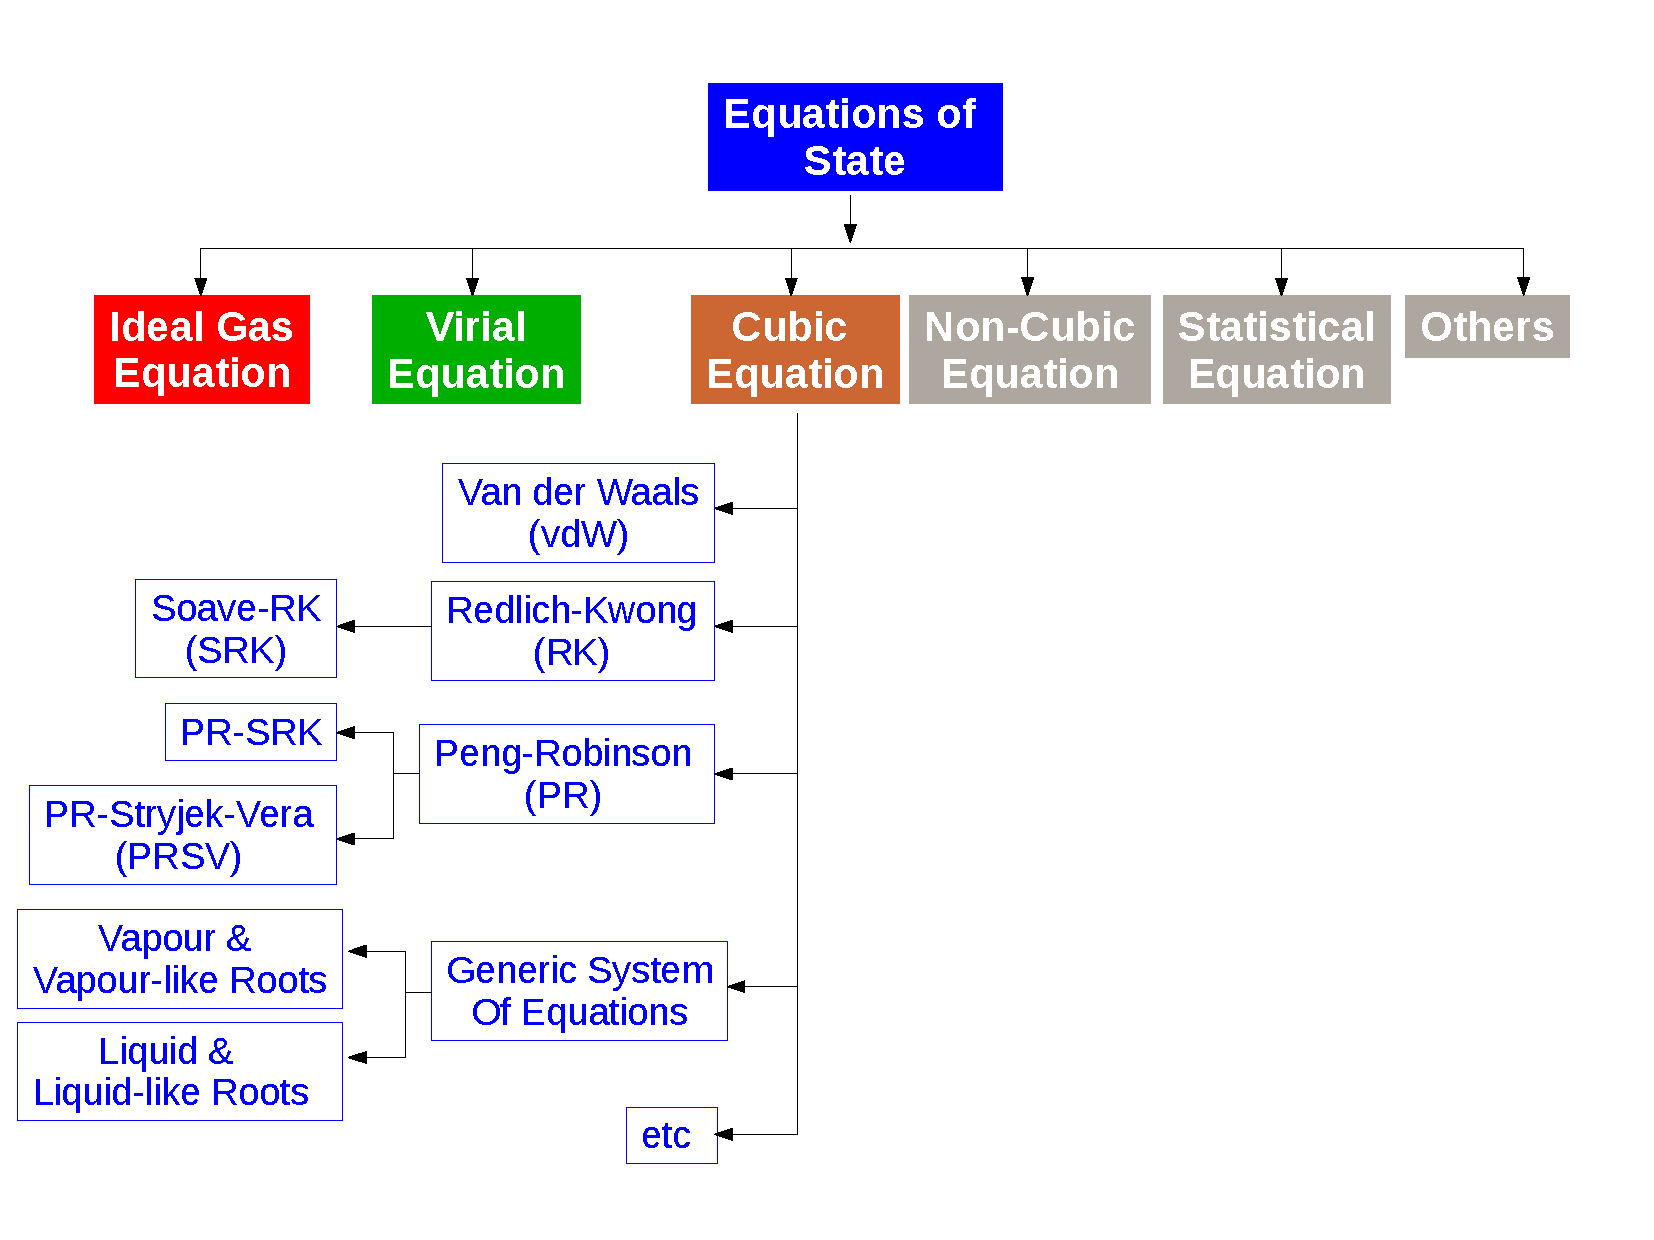
\includegraphics[width=0.9\columnwidth,clip]{./../Pics/ListEOS}
        \end{center}
      \end{figure}}
\end{frame}
\normalsize


%%%
%%% SUBSECTION
%%%
\subsection{Virial EOS}

%%%
%%% Slide
%%%
\scriptsize
\begin{frame}
 \frametitle{Virial Expansion}
   \begin{columns}
    \begin{column}[l]{0.5\linewidth}
      \begin{enumerate} \scriptsize
        \item<1-> $\left(PV\right)$ along an isotherm can be expressed as function of {\bf P} by a \textcolor{blue}{power series},
           \visible<1->{\begin{displaymath}
             \left(PV\right) = a + bP + cP^{2} + dP^{3} + \cdots
           \end{displaymath}}
        \item<2-> Defining $b=aB^{\prime}$, $c=aC^{\prime}$, $d=aD^{\prime}$, $\cdots$, then
           \visible<2->{\begin{equation}\label{Mod3:VirialEoS1}
             \left(PV\right) = a\left( 1 + B^{\prime}P + C^{\prime}P^{2} + D^{\prime}P^{3} + \cdots\right) 
           \end{equation}}
        \item<2-> $B^{\prime}$, $C^{\prime}$ and $D^{\prime}$ are constants, characteristic for each chemical species and temperature-dependent $\left(\text{i.e.,} B^{\prime}=B^{\prime}(T), C^{\prime}=C^{\prime}(T)\right)$  
        \item<3-> In the limit case -- $P\rightarrow 0$, \textcolor{blue}{$\left(PV\right)$ for all gases}:\\
           \begin{displaymath}
              \visible<3->{\textcolor{blue}{\left(PV\right)^{\star} =}} 
                   \begin{cases}
                      \visible<3->{a = f\left(T\right)} \\
                      \visible<4->{\textcolor{blue}{a= RT}}\\ 
                   \end{cases}
           \end{displaymath}
           \visible<4->{where $R$ is a proportionally constant, i.e.,  universal gas constant.}
        \item<5-> At this limiting case, $\left(PV\right)_{T}^{\star} = R \times 273.16$. 
      \end{enumerate}
    \end{column}
    \begin{column}[l]{0.5\linewidth}\scriptsize
     \begin{enumerate}\setcounter{enumi}{5}
       \item<6->For \textcolor{blue}{ideal gasses}, pressure is sufficiently small $\left(P\rightarrow 0\right)$. 
       \item<6-> This means that the molecules are separated by infinite distances, and therefore the \textcolor{blue}{intermolecular forces approaches zero}. 
     \end{enumerate}
      \visible<3->{\begin{figure}%
        \begin{center}
          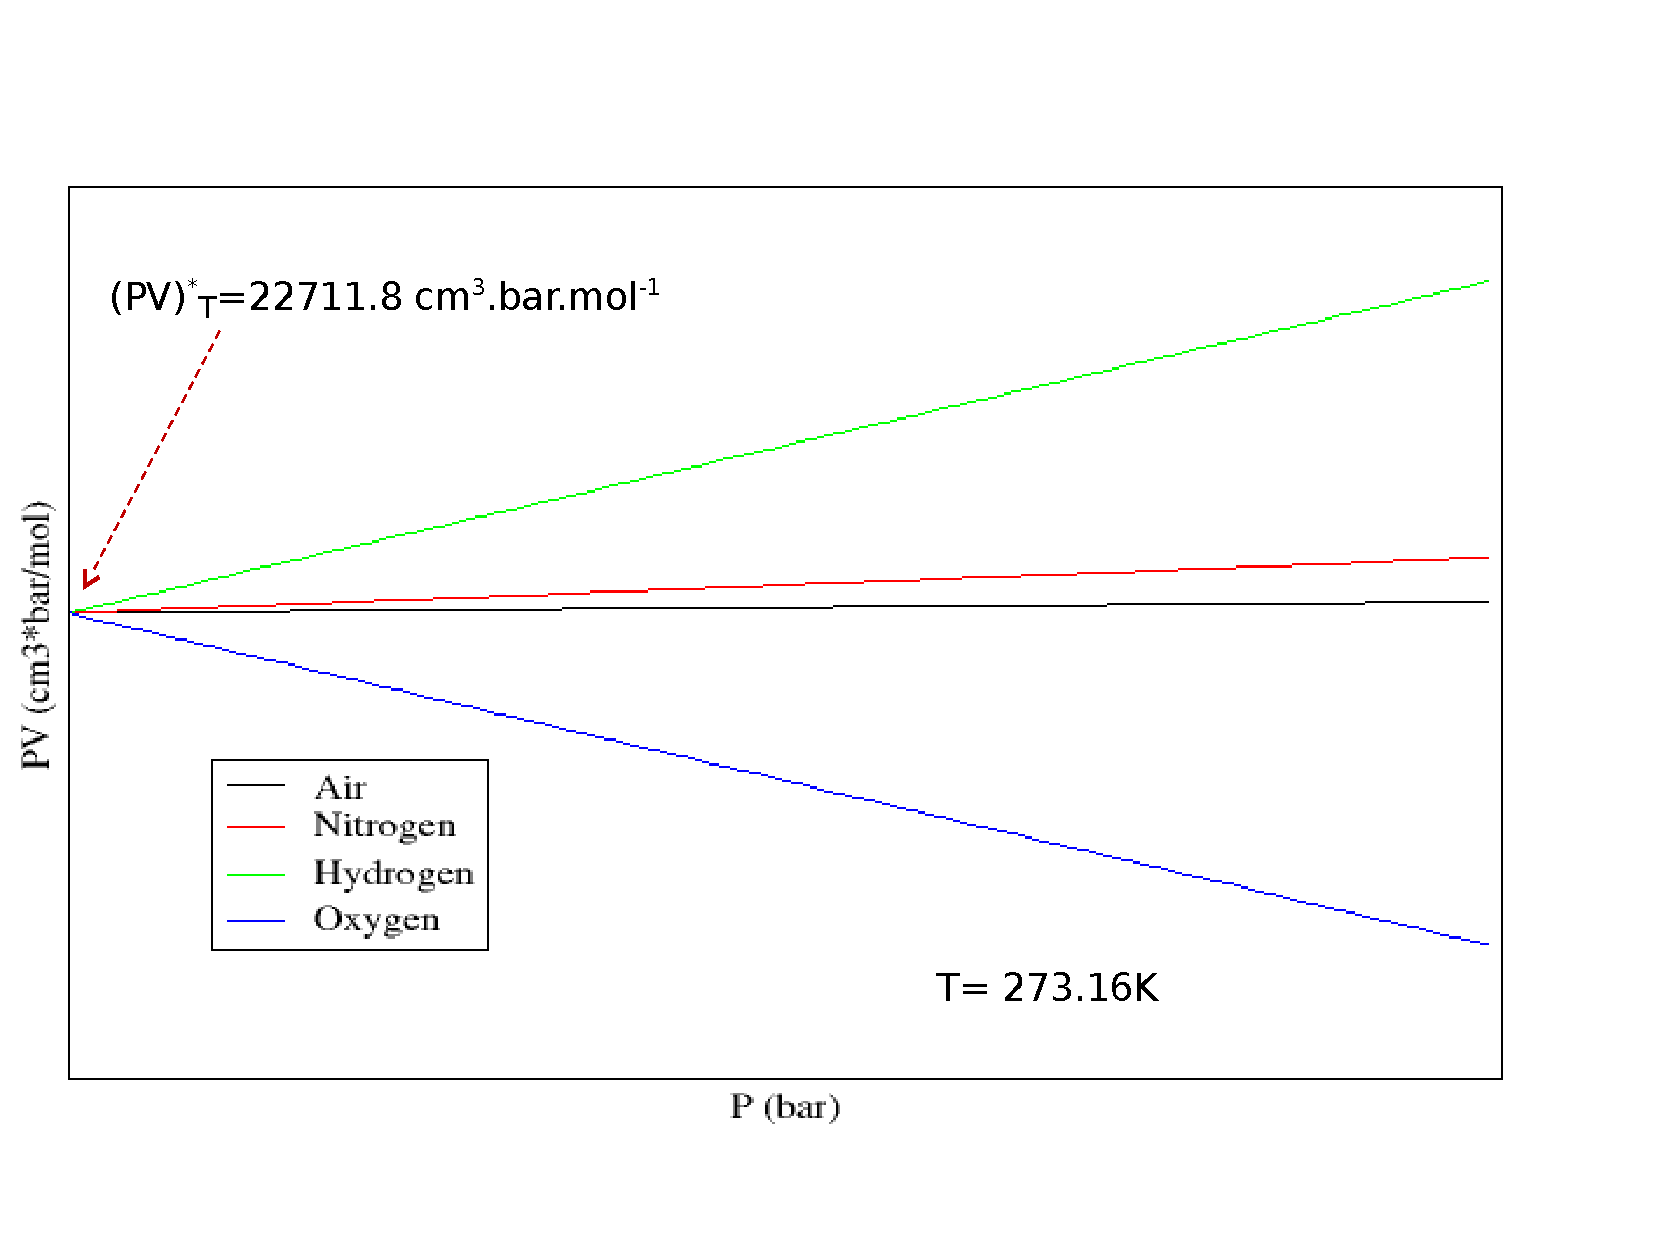
\includegraphics[width=1.05\columnwidth,clip]{./../Pics/Virial_EOS}
        \end{center}
      \end{figure}}
    \end{column}
  \end{columns}

\end{frame}
\normalsize


%%%
%%% Slide
%%%
\scriptsize
\begin{frame}
 \frametitle{Compressibility Factor -- $Z$}
   \begin{enumerate}\setcounter{enumi}{7}\scriptsize
     \item<1-> The {\it Virial expansion} is considered the only EOS based on rigorous mathematical derivation. It can also be derived from statistical mechanics leading to physical  significance of the virial coefficients;
     \item<2->The original form of the Virial EOS (Eqn.~\ref{Mod3:VirialEoS1}) can be rewritten as
        \begin{equation}\label{Mod3:VirialEoS2}
            \visible<2->{\frc{PV}{RT}} \visible<3->{ = \textcolor{red}{Z}} = \visible<2->{1 + B^{\prime}P + C^{\prime}P^{2} + D^{\prime}P^{3} + \cdots}
        \end{equation}
     \item<4-> \textcolor{red}{$Z$} is the \textcolor{blue}{compressibility factor} and is commonly used to estimate the deviation from ideal gas behaviour.
     \item<5->Therefore, the Virial EOS can be represented by 2 main forms:
        \begin{equation}
          Z = \frc{PV}{RT} =
             \begin{cases}
                1 + \textcolor{blue}{\frc{B}{V}} + \textcolor{red}{\frc{C}{V^{2}}} + \textcolor{purple}{\frc{D}{V^{3}}} + \cdots \\
                \visible<6->{1 + \blue{B^{\prime}P} + \red{C^{\prime}P^{2}} + \purple{D^{\prime}P^{3}} + \cdots} \\
                \visible<7->{1 + \blue{\frc{B}{RT}P} + \red{\frc{C-B^{2}}{\left(RT\right)^{2}}P^{2}} + \purple{\frc{D-3BC+2B^{2}}{\left(RT\right)^{3}}P^{3}} + \cdots}
             \end{cases}
        \end{equation}
     \item<8-> Thus, for real cases
        \begin{equation}
          \visible<8->{Z = \frc{PV}{RT} =}
             \begin{cases}
                \visible<8->{1 + \blue{B^{\prime}P} = 1 + \blue{\frc{BP}{RT}} \hspace{2.6cm} \Rightarrow\;\; \text{Low-Moderate pressures -- P}<\text{15 bar}}\\
                \visible<9->{1 + \blue{B^{\prime}P} + \red{C^{\prime}P^{2}}  = 1 + \blue{\frc{BP}{RT}} + \red{\frc{C-B^{2}}{\left(RT\right)^{2}}P^{2}}\;\;\Rightarrow\;\; \text{High pressures \red{but} below the } P_{c}}
             \end{cases}
        \end{equation}
             
   \end{enumerate}
\end{frame}
\normalsize


%%%
%%% SUBSECTION
%%%
\subsection{Cubic EOS}

%%%
%%% Slide
%%%
\scriptsize
\begin{frame}
 \frametitle{Generic Cubic EOS}
    \begin{enumerate}\scriptsize
      \item<1-> The simplest equations able to represent both \blue{liquid} and \blue{vapour} phases behaviour but \red{not} for two-phase condition;
      \item<2-> They are designed to be used in a wide range of temperature and pressure;
      \item<3-> General format of a cubic equation on $V$,
         \begin{equation}\label{Mod3:GenCubicEqn}
            \visible<3->{
             P = \frc{RT}{V-b} - \frc{\theta\left(V-\eta\right)}{\left(V-b\right)\left(V^{2}+\kappa V + \lambda\right)}
            }
         \end{equation}
         \visible<3->{Where $b$, $\theta$, $\kappa$, $\lambda$ and $\eta$ are parameters that depend on \blue{T} and \blue{composition} (for mixtures).}
      \item<4-> If $\eta=b$, $\theta=a(T)$,$\kappa=\left(\epsilon+\sigma\right)b$ and $\lambda=\epsilon\sigma b^{2}$, we can define a generic cubic equation of state,
           \visible<4->{\begin{equation}\label{Mod3:GenCubicEOS}
              P = \frc{RT}{V-b} - \frc{a(T)}{\left(V-\epsilon b\right)\left(V+\sigma b\right)}
           \end{equation}
           where $\epsilon$ and $\sigma$ are constants.}
       \item<5-> $a(T)$ and $b$ are specific for chemical species and defined as,
           \visible<5->{\begin{displaymath} 
             a(T) = \Psi\frc{\alpha(T)R^{2}T_{c}^{2}}{P_{c}}\;\;\;\text{ and }\;\;\; b=\Omega\frc{R T_{c}}{P_{c}}
           \end{displaymath}
           $\Psi$ and $\Omega$ are constants and may vary for different cubic EOS.} 
    \end{enumerate}
\end{frame}
\normalsize

%%%
%%% Slide
%%%
\scriptsize
\begin{frame}
 \frametitle{Cubic Equations of State}
    \visible<1->{\begin{block}{van der Waals}
        If we set $\eta=b$, $\theta=a$ and $\kappa=\lambda=0$, Eqn.~\ref{Mod3:GenCubicEqn} reduces to 
        \begin{equation}\label{Mod3:vdWEOS}
              P = \frc{RT}{V-b} - \frc{a}{V^{2}}
        \end{equation}
        with $a=\frc{27 R^{2}T_{c}^{2}}{64 P_{c}}$ and $b=\frc{R T_{c}}{8 P_{c}}$.
    \end{block}}    

    \visible<2->{\begin{block}{Redlich-Kwong}
        \begin{equation}\label{Mod3:vdWEOS}
              P = \frc{RT}{V-b} - \frc{a}{\sqrt{T_{r}}\left(V + b\right)V}
        \end{equation}
       with $a = 0.42748\frc{R^{2}T_{c}^{2}}{P_{c}}$ and $b=0.08664\frc{R T_{c}}{P_{c}}$.
    \end{block}}    

\end{frame}
\normalsize

%%%
%%% Slide
%%%
\scriptsize
\begin{frame}
 \frametitle{Cubic Equations of State}
    \visible<1->{\begin{block}{Soave-Redlich-Kwong}
        \begin{equation}\label{Mod3:SRKEOS}
              P = \frc{RT}{V-b} - \frc{a\alpha}{V\left(V+b\right)}
        \end{equation}
        with $\alpha = \left[1+\gamma\left(1-\sqrt{T_{r}}\right)\right]^{2}$ and $\gamma=0.480+1.574\omega-0.176\omega^{2}$, where $T_{r}=\frc{T}{T_{c}}$.
    \end{block}}    

    \visible<2->{\begin{block}{Peng-Robinson}
        \begin{equation}\label{Mod3:PREOS} 
              P = \frc{RT}{V-b} - \frc{a\alpha}{V\left(V+b\right)+b\left(V-b\right)}
        \end{equation}
       with  $\gamma=0.37464+1.54226\omega-0.26992\omega^{2}$, $a=0.45724\frc{R^{2}T_{c}^{2}}{P_{c}}$ and $b=0.07780\frc{R T_{c}}{P_{c}}$
    \end{block}}    

\end{frame}
\normalsize


%%%
%%% Slide
%%%
%\scriptsize
\begin{frame}
 \frametitle{Cubic Equations of State}
   \visible<1->{\begin{block}{Theorem of Corresponding States (TCS)}
     \blue{$\lq$All fluids, when compared at the same reduced temperature $\left(T_{r}\right)$ and pressure $\left(P_{r}\right)$, have approximately the same compressibility factor $(Z)$, and all deviate from ideal behaviour to about the same degree.'}
     \begin{displaymath}
           T_{r}\equiv\frc{T}{T_{c}} \hspace{3cm} P_{r} \equiv \frc{P}{P_{c}}
     \end{displaymath}
   \end{block}}
   \begin{enumerate}
     \item<2-> TCS is exact for \blue{simple fluids}, e.g., $Ar$, $Kr$ and $Xe$.
     \item<3-> However, larger deviations are observed for \blue{more complex fluids}. 
     \item<4-> Thus, an \red{acentric factor $\left(\omega\right)$} was introduced,
         \begin{displaymath}
            \omega \equiv 1 -\log\left(P^{\text{sat}}_{r}\right)_{T_{r}=0.7}
         \end{displaymath}
         where $\left(P_{r}^{\text{sat}}\right)_{T_{r}=0.7}$ is the reduced vapour pressure at reduced temperature of 0.7. At $T_{r}=0.7$, $\omega=0$ for $Ar$, $Kr$ and $Xe$.
     \item<5-> $\omega$ can be determined for any fluid based on $T_{c}$, P$_{c}$ and a vapour-pressure measurement at $T_{r}=0.7$. 
   \end{enumerate}

\end{frame}
\normalsize


%%%
%%% Slide
%%%
%\scriptsize
\begin{frame}
 \frametitle{Cubic Equations of State}
    \visible<1->{\begin{block}{Vapour $\&$ Vapour-like Roots}
      \begin{displaymath}
        Z= 1 + \beta - q\beta \frc{Z - \beta} {\left(Z+\varepsilon\beta\right)\left(Z+\sigma\beta\right)}
      \end{displaymath}
      with $\beta=\Omega\frc{P_{r}}{T_{r}}$ and $q=\frc{\Psi\alpha}{\Omega T_{r}}$
    \end{block}}


    \visible<2->{\begin{block}{Liquid $\&$ Liquid-like Roots}
      \begin{displaymath}
        Z= 1 + \beta + \left(Z + \epsilon\beta\right)\left(Z+\sigma\beta\right)\left(\frc{1+\beta-Z}{q\beta}\right)
      \end{displaymath}
    \end{block}}

    \visible<3->{Iterative method to solve the expressions above, using $Z=1$ as the initial guess.}


\end{frame}
\normalsize



%%%
%%% Slide
%%%
%\scriptsize
\begin{frame}
 \frametitle{Cubic Equations of State -- Parameters}
    \begin{center}
       \begin{tabular}{| l | c c c c c| }
       \hline
          {\bf EOS}  & {\bf $\alpha$} & {\bf $\sigma$}  & {\bf $\varepsilon$} & {\bf $\Omega$} & {\bf $\Psi$ } \\
       \hline
            vdW      & 1              & 0               & 0                  & 1/8            & 27/64          \\
            RK       & T$_{r}^{-1/2}$  & 1                & 0                  & 0.08664       & 0.42748        \\
           SRK       &$\alpha_{\text{SRK}}$& 1            & 0                   & 0.08664       & 0.42748        \\
            PR       &$\alpha_{\text{PR}}$& 1+$\sqrt{2}$   & 1-$\sqrt{2}$        & 0.07780        & 0.45724  \\
       \hline
       \end{tabular}
    \end{center}
\begin{eqnarray}
\alpha_{\text{SRK}} &=& \left[ 1 + \left( 0.480 + 1.574 \omega - 0.176\omega^{2}\right)\left(1-\sqrt{T_{r}}\right)\right]^{2} \nonumber \\
\alpha_{\text{PR}} &=& \left[ 1 + \left( 0.37464 + 1.54226 \omega - 0.26992\omega^{2}\right)\left(1-\sqrt{T_{r}}\right)\right]^{2} \nonumber
\end{eqnarray}

\end{frame}
\normalsize

\section{Summary}

%%%
%%% Slide
%%%
%\scriptsize
\begin{frame}
 \frametitle{Summary}
   \begin{enumerate}
     \item Review of phase diagram and Gibbs rule, including
       \begin{enumerate}
         \item $PT$ and $PV$ diagrams and phase equilibrium;
         \item Critical and Triple points;
       \end{enumerate}
     \item Equations of state
       \begin{enumerate}
         \item General formulation;
         \item Parameters for cubic EOS;
         \item 2- and 3- parameters cubic EOS.
       \end{enumerate}
   \end{enumerate}
\end{frame}


\end{document}
 % Volumetric Properties of Pure Fluids

\part{Power and Refrigeration}

\part{Liquid Solutions}

\part{Fundamental Chemical Reactions}

\pagebreak

\cleardoublepage

  \begin{appendix}
\part{Appendices}
     
\chapter{Unit Conversion}


Extracted from~\cite{Balmer_Book}:\\
  \begin{tabular}{c l}
     \hspace{1cm} & R.T. Balmer \\
                  & Modern Engineering Thermodynamics \\
                  & Academic Press, 2011  \\
  \end{tabular}


\begin{list}{\bf Example \arabic{qcounter}:~}{\usecounter{qcounter}}
%
   \item\label{Example:UnitConversion1} Calculate the volume $\left(\text{in m}^{3}\right)$ of 1 kg of hydrogen gas $\left(\text{molecular mass of 2.016 kg.kgmol}^{-1}\right)$ at 27$^{\circ}$C and 1 bar. Assume ideal gas behaviour.
     \begin{description}
        \item[Solution:] We can use the ideal gas equation of state to calculate the volume of H$_{2}$ gas,
           \begin{displaymath}
              V = \frc{nRT}{P},
           \end{displaymath}
           where $n = m/MW$ is the number of moles, $m$, $MW$ and $R$ are the mass, molecular mass, and universal gas constant, respectively. We should be able to replace the variables with their values,
           \begin{eqnarray}
              V &=& \frc{nRT}{P} = \frc{ \frc{m}{MW} R T }{ P } \nonumber \\
                &=& \frc{ \frc{ 1\text{ kg}}{ 2.016\text{ kg.kgmol}^{-1}}\;\; 0.08314\frc{\text{bar.m}^{3}}{\text{kgmol.K}}\;\; ( 27 + 273.15)\text{ K}}{ 1 \text{ bar}},\nonumber
           \end{eqnarray}
           It is clear that the units above are consistent and can be easily eliminated resulting in m$^{3}$,
           \begin{eqnarray}
              V &=& \frc{ \frc{ 1\cancel{\text{ kg}}}{ 2.016\text{ \cancel{kg}.}\cancel{\text{kgmol}^{-1}}}\;\; 0.08314\frc{\text{\cancel{bar}.m}^{3}}{\text{\cancel{kgmol}.\cancel{K}}}\;\; ( 27 + 273.15)\cancel{\text{ K}}}{ 1 \text{ \cancel{bar}}},\nonumber \\
                &=& 12.3782\text{ m}^{3}.\nonumber
           \end{eqnarray}

     \end{description}
%
   \item\label{Example:UnitConversion2}  Liquid water at 0.70 bar is transferred from a condenser to a boiler through a pump. The pressure in the exit of the pump is 25 bar. Assuming that the water undertakes an isentropic (\ie constant entropy) compression, calculate the specific enthalpy of the water after the pump. Consider that the liquid water as incompressible and
       \begin{displaymath}
          dh = Tds + vdP,
       \end{displaymath}
where h, s, v are specific enthalpy (kJ/kg), entropy (kJ/(kg.K)) and volume (m$^{3}$.kg).
     \begin{description}
        \item[Solution:] If the process is isentropic, therefore $ds=0$ and the fundamental thermodynamic relation is simplified to,
       \begin{displaymath}
          dh = vdP \Longrightarrow h_{2} - h_{1} = v\left(P_{2}-P_{1}\right),
       \end{displaymath}
      or summarising,
       \begin{center}
         \begin{tabular}{c| c c c}
            State  & $P$ (bar)  & $h$ (kJ/kg) & $v$ $\left(\text{m}^{3}\text{.kg}\right)$ \\
\hline
              1    &   0.70    &  376.70   &  1.0360$\times$10$^{-3}$                 \\
              2    &  25.0    & \red{h$_{2}$}& 1.0360$\times$10$^{-3}$ 
         \end{tabular}
       \end{center}
       Values of {\it State 1} were obtained from the water saturated table (Appendix~\ref{Appendix:Saturated_SH_Tables}). Note that as the fluid is assumed incompressible there is no variation in the volume, $v_{1}=v_{2}$.
       \begin{eqnarray}
         h_{2} &=& h_{1} = v\left(P_{2}-P_{1}\right) \nonumber \\
              &=& 376.70\frc{\text{kJ}}{\text{kg}} + 1.0360\times 10^{-3}\frc{\text{m}^{3}}{\text{kg}}\;\left(25 - 0.70\right)\text{ bar}  \nonumber\\
              &=& 376.70\frc{\text{kJ}}{\text{kg}} + 0.02517 \frc{\text{m}^{3}.\text{bar}}{\text{kg}} \nonumber
       \end{eqnarray}
       It is clear that the units in the two terms of the r.h.s. of the equation contain distinct units that \underline{can not} be summed up. Therefore, we need to convert $\left[\text{m}^{3}.\text{bar}\right]$ to $[\text{kJ}]$. Bearing in mind that 1 J = 1 N.m = 1 kg.m$^{2}$.s$^{-2}$, we first can convert $\left[\text{m}^{3}.\text{bar}\right]$ to $\left[\text{kg.m}^{2}.\text{s}^{-2}\right]$
       \begin{displaymath}
          1 \cancelto{\blue{\text{m}^{2}}}{\text{m}^{3}}.\red{\cancel{\text{bar}}} \times \frc{\red{10^{5}\cancel{\text{ Pa}}}}{\red{1 \cancel{\text{ bar}}}} \times \frc{\red{ 1 \text{ kg}/\left(\cancel{\blue{\text{m}}}.\text{s}^{2}\right)}}{\red{ 1 \cancel{\text{ Pa}}}} = 10^{5} \frac{\text{kg.m}^{2}}{\text{s}^{2}}
       \end{displaymath}
       Now, replacing the converted $\left[\text{m}^{3}.\text{bar}\right]$ term in the r.h.s. of the expression for $h_{2}$,
       \begin{eqnarray}
         h_{2} &=& 376.70\frc{\text{kJ}}{\text{kg}} + 0.02517 \frc{\text{m}^{3}.\text{bar}}{\text{kg}} \nonumber \\
              &=& 376.70\frc{\text{kJ}}{\text{kg}} + 0.02517 \frc{\cancel{\left(\text{m}^{3}.\text{bar}\right)}}{\text{kg}} \times \frc{10^{5} \frac{\text{kg.m}^{2}}{\text{s}^{2}}}{1 \cancel{\left(\text{m}^{3}.\text{bar}\right)}} \nonumber \\
              &=& 376.70\frc{\text{kJ}}{\text{kg}} + 2517 \frc{\cancelto{\red{\text{J}}}{\frac{\text{kg.m}^{2}}{\text{s}^{2}}}}{\text{kg}}\nonumber\\
              &=& 376.70\frc{\text{kJ}}{\text{kg}} + 2517 \frc{\text{J}}{\text{kg}} \nonumber
       \end{eqnarray}
       We still \underline{can not} sum the two terms in the r.h.s., as the first term involves $\left[\text{kJ/kg}\right]$ whereas the second term is $\left[\text{J/kg}\right]$, therefore
       \begin{eqnarray}
         h_{2} &=& 376.70\frc{\text{kJ}}{\text{kg}} + 2517 \frc{\text{J}}{\text{kg}} \nonumber\\
              &=& 376.70\frc{\text{kJ}}{\text{kg}} + 2517 \frc{\cancel{\text{J}}}{\text{kg}} \red{\times \frc{1\text{ kJ}}{1000 \cancel{\text{J}}}}\nonumber\\
              &=& 379.22 \frc{\text{kJ}}{\text{kg}}\nonumber
       \end{eqnarray}
       


     \end{description}
%
\end{list}

  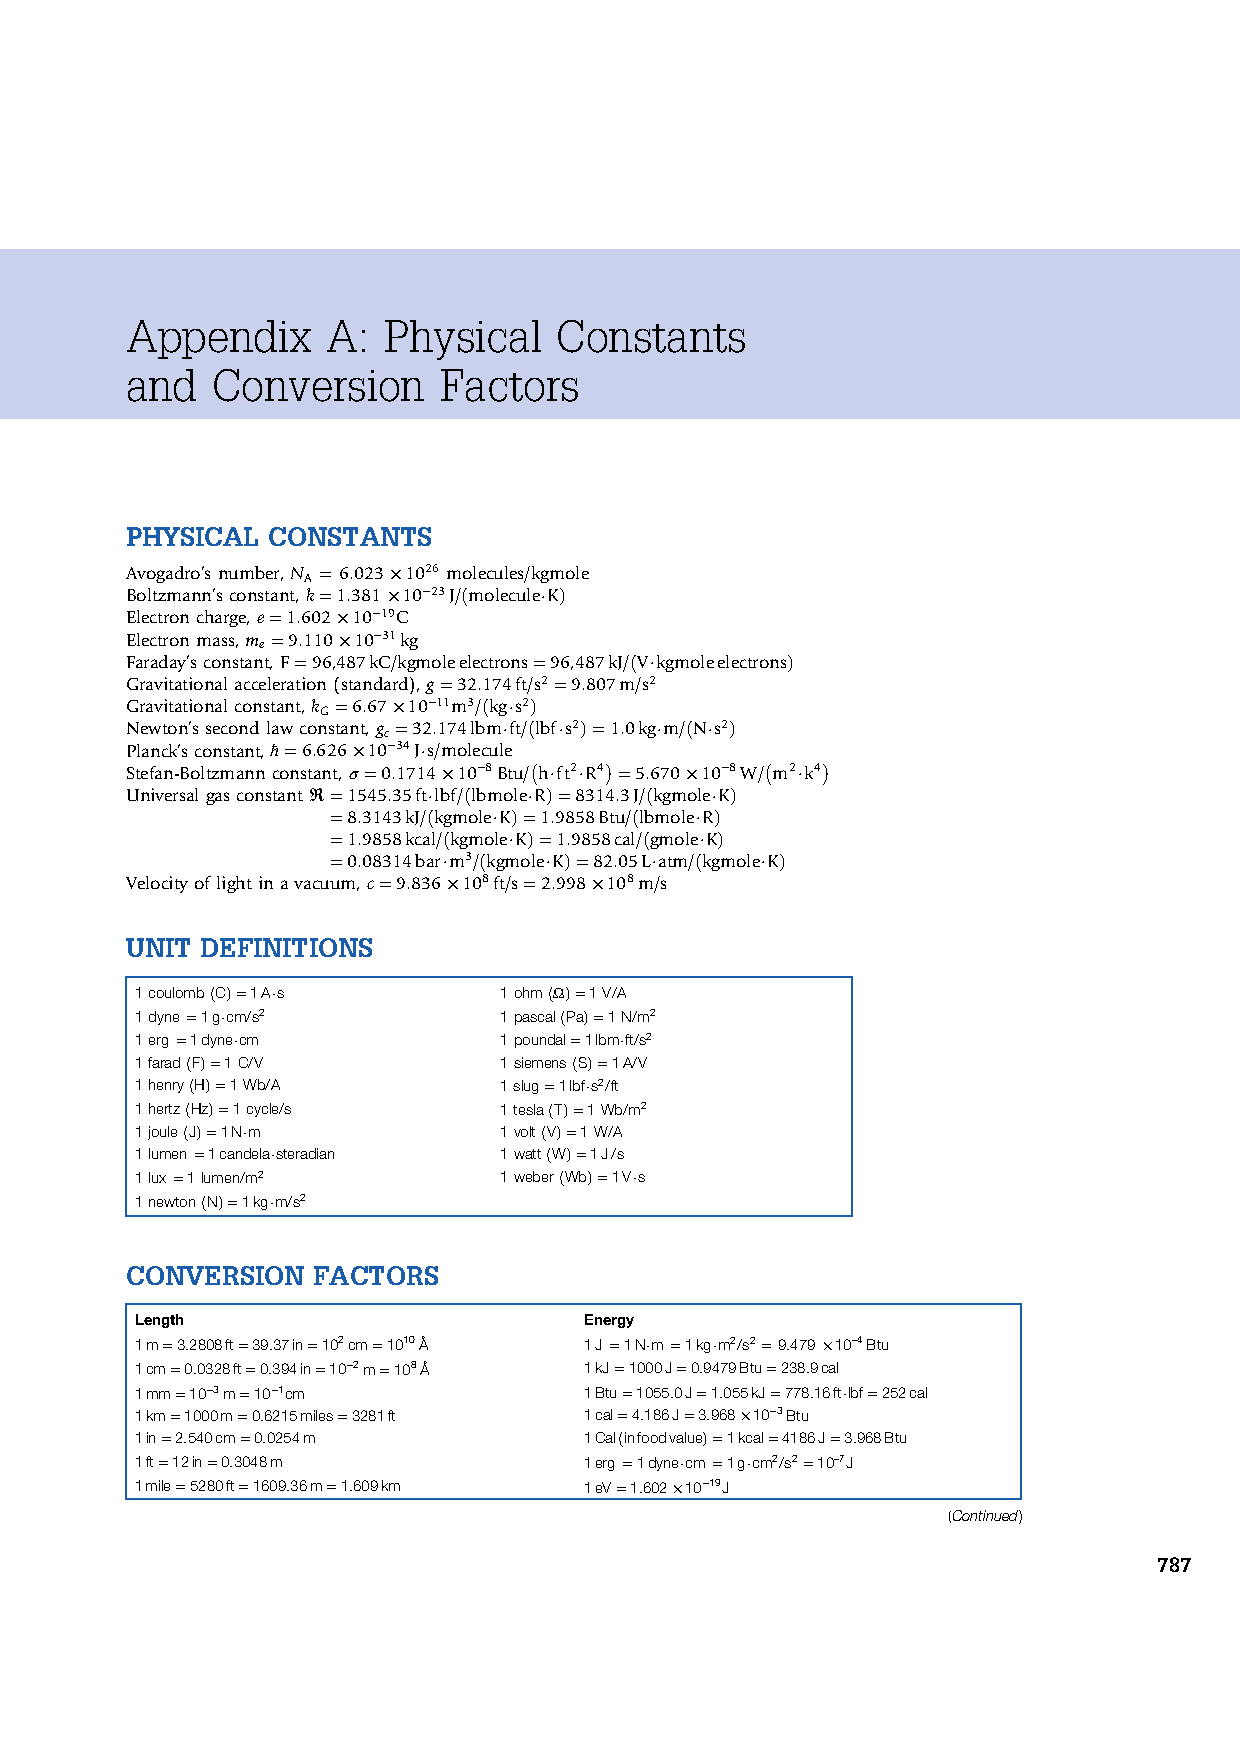
\includepdf[scale=1,pages=-,pagecommand={}, fitpaper]{./../Pics/ChemEng_UnitConv.pdf}

     
\chapter{Table of Properties of Saturated and Superheated Fluids}

Extracted from~\cite{Moran_Book}:\\
  \begin{tabular}{c l}
     \hspace{1cm} & M.J. Moran and H.N. Saphiro \\
                  & Fundamentals of Engineering Thermodynamics \\
                  & John Wiley $\&$ Sons, 5$^{\text{th}}$ Edition  \\
  \end{tabular}

  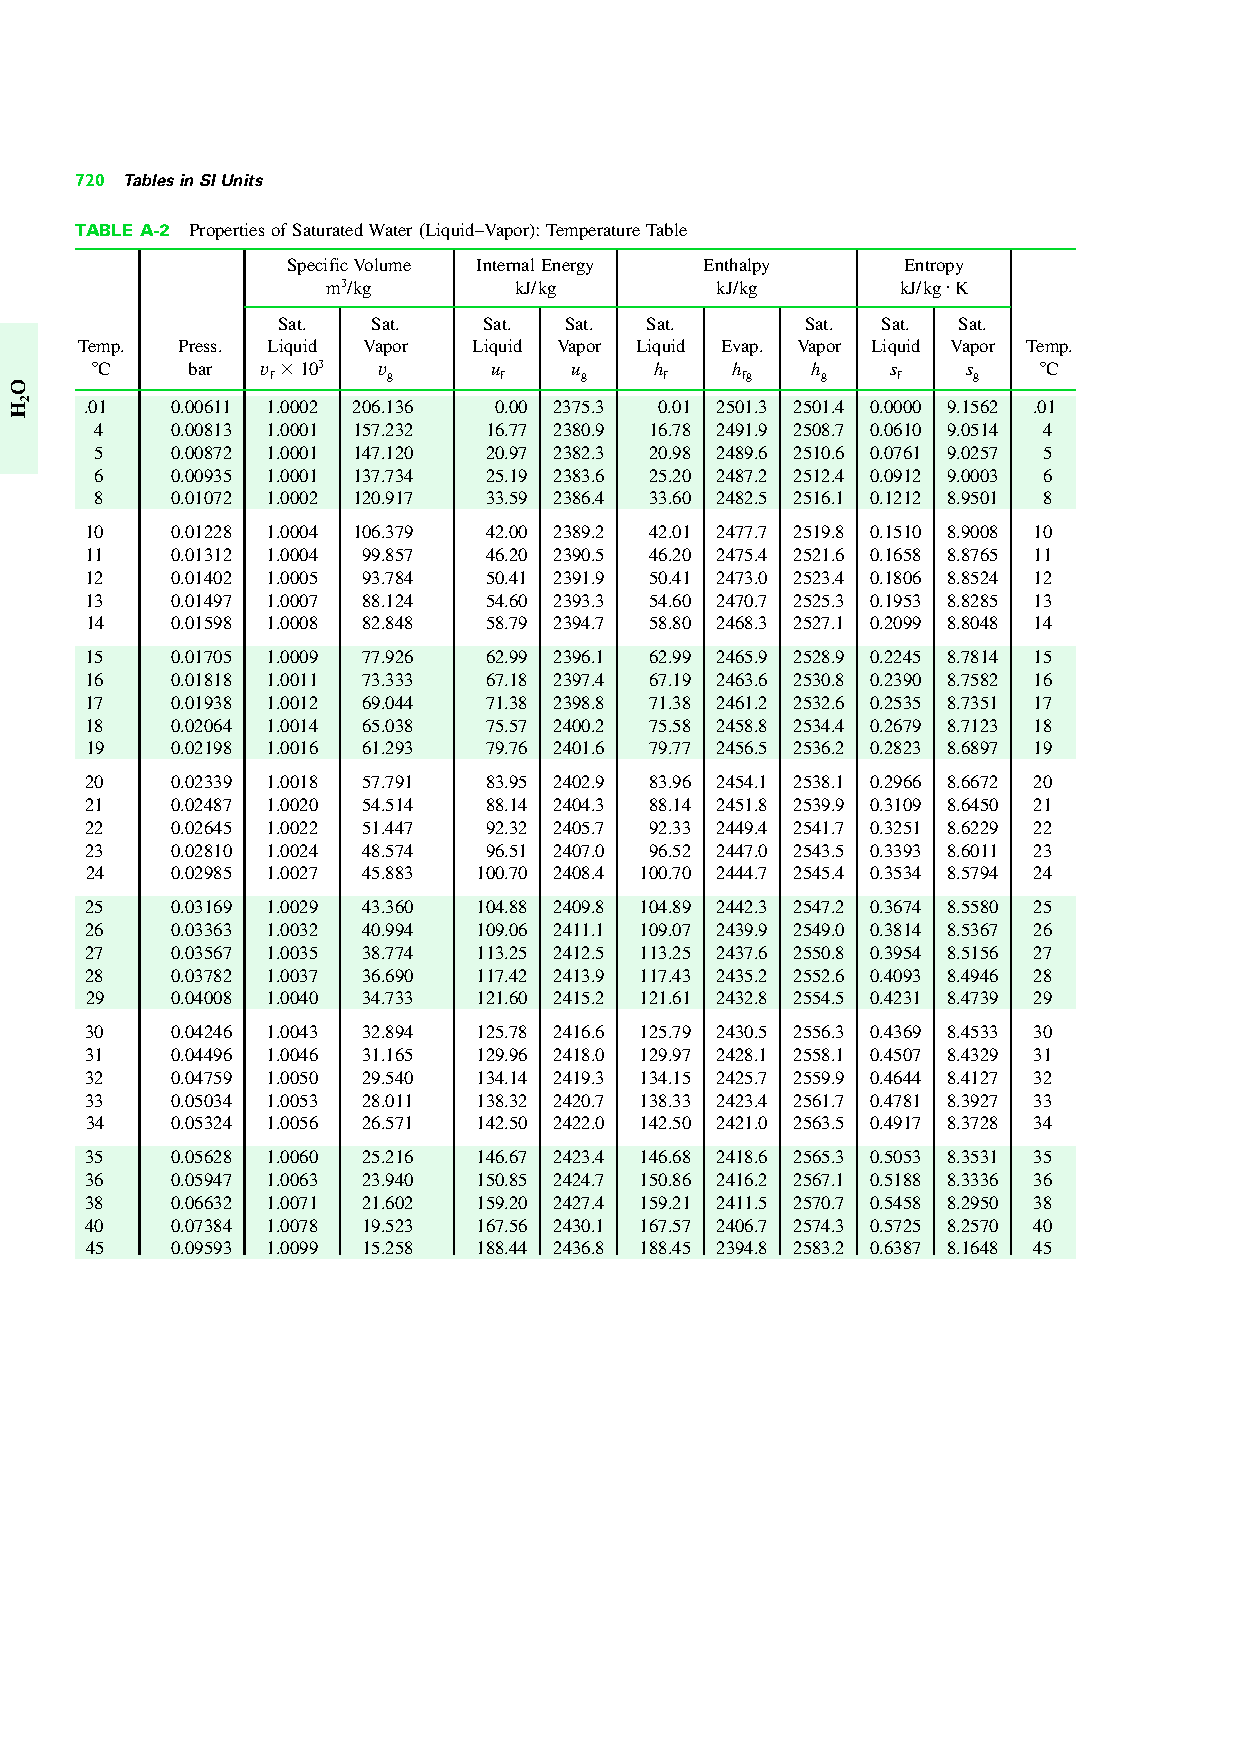
\includepdf[scale=1,pages=-,pagecommand={}, fitpaper]{./Pics/ChemEng_AllTables.pdf}

     
\chapter{Summary of Logarithms and Exponential Properties}
{\it This is not examinable} -- it is here so that you can see where some of the notations, operations and results of earlier sections come from. 

%%%
%%% EXPONENTS
%%%
\section{Exponents}
Assuming that $a$, $b$, $m$ and $n$ are real numbers, the following properties of exponents hold:
\begin{center}
  \begin{tabular}{||c l | c l ||}
    \hline\hline
     1 & $a^{m}a^{n} = a^{m+n}$ & 6 & $\frc{a^{m}}{a^{n}} = a^{m-n}$, $\forall a\neq 0$ \\
     2 & $\left(a^{m}\right)^{n} = a^{mn}$ & 7 &  $\left(ab\right)^{m} = a^{m}b^{m}$ \\
     3 & $\left(\frc{a}{b}\right)^{m} = \frc{a^{m}}{b^{m}}$, $\forall b\neq 0$ & 8 & $a^{-m}=\frc{1}{a^{m}}$, $\forall a\neq 0$ \\
     4 & $a^{1/n} = \sqrt[n]{a}$ & 9 & $a^{0} = 1$, $\forall a\neq 0$ \\
     5 & $a^{m/n} = \sqrt[n]{a^{m}} = \left(\sqrt[n]{a}\right)^{m}$ & & \\ 
    \hline\hline
  \end{tabular}
\end{center}


%%%
%%% LOGARITHMS
%%%
\section{Logarithms}
Let's define $y = \log_{a}x$ if ({\it and only if}) $x=a^{y}$, $\forall a>0$. Given the {\it Euler number}, $e$,
\begin{displaymath}
e = \sum\limits_{n=0}^{\infty}\frc{1}{n!}\sim 2.71828
\end{displaymath}
we can define $\ln x = \log_{e}{x}$, referred as the natural logarithm. The following properties of logarithms hold:
\begin{center}
  \begin{tabular}{||c l | c l||}
     \hline\hline
       1  & $\log_{a}b = \frc{\log_{10}{a}}{\log_{10}{b}}$ & 1' & $\log_{a}b = \frc{\ln{a}}{\ln{b}}$\\
     \hline
       2  & $\log_{a}{xy} = \log_{a}{x}+\log_{a}{y}$ & 2' &$\ln{xy} = \ln{x}+\ln{y}$  \\
     \hline
       3  & $\log_{a}{\frc{x}{y}} = \log_{a}{x}-\log_{a}{y}$ & 3' & $\ln{\frc{x}{y}} = \ln{x}-\ln{y}$ \\
     \hline
       4  & $\log_{a}{x^{y}} = y\cdot\log_{a}{x}$ & 4' & $\ln{x^{y}} = y\cdot\ln{x}$ \\
     \hline
       5  & $\log_{a}{a^{x}} = x$ & 5' & $\ln{e^{x}} = x$ \\
     \hline
       6  & $a^{\log_{a}{x}} = x$   & 6' & $e^{\ln{x}} = x$ \\
     \hline
       7  & $\log_{a}{a} = 1$, $\forall a>0$ & 7' & $\ln{e} = 1$ \\ 
     \hline
       8  & $\log_{a}1 = 0$, $\forall a > 0$ & 8' & $\ln{1} = 0$ \\
     \hline\hline
  \end{tabular}  
\end{center}

     
\chapter{Calculus' Background for Thermodynamics}\label{Appendix_Calculus}
{\it This is not examinable} -- it is here so that you can see where some of the notations, operations and results of earlier sections came from. Details of the contents of this Appendix can be found in \cite{Leithold_Book,Kallo_1955,Strang_Book} or in any {\it Calculus} text-book.
\bigskip

%%%
%%% SECTION
%%%
\section{Vector Calculus}

The operator {\it del} (or {\it nabla}),\index{{\it del} ($\nabla$) operator}\index{{\it nabla} ($\nabla$) operator}\index{$\nabla$}
\begin{displaymath}
  \nabla \equiv \left(\frc{\partial}{\partial x}, \frac{\partial}{\partial y}, \frac{\partial}{\partial z}\right)
\end{displaymath} 
is both a vector and a differential operator and can be used to define,
\begin{enumerate}
%
  \item Gradient: operates on a scalar field $\phi$, e.g., $T$, $\rho$, $\cdots$\index{Gradient}
     \begin{displaymath}
        \text{grad}\phi \equiv \nabla\phi \equiv \left(\frc{\partial\phi}{\partial x}, \frac{\partial\phi}{\partial y}, \frac{\partial\phi}{\partial z}\right)
     \end{displaymath}
%
  \item Divergence: operates on a vector field  $\theta = \left(\theta_{x}, \theta_{y}, \theta_{z}\right) $, e.g., velocity field.\index{Divergence}
     \begin{displaymath}
        \text{div}\theta \equiv \nabla\cdot\theta \equiv \frc{\partial\theta_{x}}{\partial x} + \frac{\partial\theta_{y}}{\partial y} + \frac{\partial\theta_{z}}{\partial z}
     \end{displaymath}
%
  \item Curl: operates on a vector field  $\theta = \left(\theta_{x}, \theta_{y}, \theta_{z}\right)$,\index{Curl}
     \begin{displaymath}
        \text{curl}\theta \equiv \nabla\times\theta \equiv \begin{pmatrix} i & j & k \\ \frc{\partial}{\partial x} & \frc{\partial}{\partial y} & \frc{\partial}{\partial z} \\ \theta_{x} & \theta_{y} & \theta_{z} \end{pmatrix}
     \end{displaymath}
%
   \item Laplacian: operates on a scalar field $\phi$,\index{Laplacian}
      \begin{displaymath}
         \text{div}\left(\text{grad}\phi\right) \equiv \nabla\cdot\nabla\phi \equiv \nabla^{2}\phi \equiv \frc{\partial^{2}\phi}{\partial x^{2}} + \frc{\partial^{2}\phi}{\partial y^{2}} + \frc{\partial^{2}\phi}{\partial z^{2}}
      \end{displaymath}
%
\end{enumerate}


%%%
%%% SECTION
%%%
\section{Some Basic Derivatives/Integration Operations}

\begin{center}
  \begin{tabular}{|| l l | l l ||}
    \hline\hline
       {\bf f(x)}  & {\bf f'(x)}  & {\bf f(x)}  & {\bf f'(x)}  \\
    \hline\hline
       $x^{n}$      &  $nx^{n-1}$   & $\ln{x}$    & $x^{-1}$      \\
       $e^{x}$      &  $e^{x}$      & $sin(x)$   & $cos(x)$     \\
       $cos(x)$    &  $-sin(x)$   & $tan(x)$    & $sec^{2}(x)$  \\
    \hline\hline
       {\bf f(x)}  &  {\bf $\int$f(x)dx} & {\bf f(x)}  &  {\bf $\int$f(x)dx} \\
    \hline\hline
       $e^{x}$      & $e^{x}+\mathcal{C}$& $x^{n}$ for $n\neq -1$ & $\frc{x^{n+1}}{n+1}+\mathcal{C}$ \\
                    &                  &                        & \\
       $1/x$ for $x\neq 0$& $\ln{|x|}+\mathcal{C}$ & $a^{x}$ for $a\neq 1$, $a>0$ & $\frc{a^{x}}{\ln{a}}+\mathcal{C}$\\
                   &                  &                         & \\
       $e^{ax}$ for $a\neq 0$  & $\frc{e^{ax}}{a}+\mathcal{C}$ & $cos(ax)$ for $a\neq0$ & $\frc{1}{a}sin(ax)+\mathcal{C}$\\
                   &                  &                        & \\
       $sin(ax)$ for $a\neq 0$ & $-\frc{1}{a}cos(ax)+\mathcal{C}$& & \\
    \hline\hline
  \end{tabular}
\end{center}

\begin{itemize}
%
  \item Derivative of a sum:
    \begin{displaymath}
       \frc{d}{dx}\left[f(x)+g(x)\right] = \frc{d}{dx}f(x) + \frc{d}{dx}g(x) = f'(x)+g'(x) 
    \end{displaymath}
%
  \item Derivative with a constant factor $c$:
    \begin{displaymath}
       \frc{d}{dx}\left[c f(x)\right] = c\frc{d}{dx}f(x) = cf'(x)
    \end{displaymath}
%
  \item Derivative of a product:
    \begin{displaymath}
       \frc{d}{dx}\left[f(x)g(x)\right] = f(x)g'(x) + f'(x)g(x)
    \end{displaymath}
%
  \item Derivative of a quotient:
    \begin{displaymath}
      \frc{d}{dx}\left[\frc{f(x)}{g(x)}\right] = \frc{g(x)f'(x)-f(x)g'(x)}{g^{2}(x)}
    \end{displaymath}
%
  \item Chain rule (or function of a function):
    \begin{displaymath}
      \frc{d}{dx}f\left[g(x)\right] = f'\left[g(x)\right]g'(x)
    \end{displaymath}
%
  \item Chain rule of a linear function:
    \begin{displaymath}
      \frc{d}{dx} \left[f(ax+b)\right] = a f'(ax+b)
    \end{displaymath}
%
  \item Integral of a function of a linear function:
    \begin{displaymath}
       \int\left[f'(ax+b)\right]dx = \frc{1}{a}f(ax+b) + \mathcal{C}
    \end{displaymath}
%
  \item Integral of a chain rule derivative:
    \begin{displaymath}
       \int\left\{f'\left[g(x)\right]g'(x)\right\}dx = f\left[g(x)\right] + \mathcal{C}
    \end{displaymath}
%
  \item Integral of a sum:
    \begin{displaymath}
      \int\left[f(x)+g(x)\right]dx = \int f(x)dx + \int g(x)dx
    \end{displaymath}
%
  \item Integral with a constant function:
    \begin{displaymath}
       \int c f(x)dx = c\int f(x)dx
    \end{displaymath}
%
  \item Integration by parts:
    \begin{displaymath}
       \int\left[f(x)g'(x)\right]dx = f(x)g(x) - \int\left[f'(x)g(x)\right]dx
    \end{displaymath}
%
  \item Definite integral (if $f'(x)$ is continuous at $a<x<b$):
    \begin{eqnarray}
       && \int\limits_{a}^{b}f(x)dx = - \int\limits_{b}^{a}f(x)dx \nonumber \\
       && \int\limits_{a}^{b}f'(x)dx = \left.f(x)\right|_{a}^{b} = \lim_{x\rightarrow b^{-}}f(x)-\lim_{x\rightarrow a^{+}}f(x)\nonumber
    \end{eqnarray}
%
  \item Substitution:
    \begin{eqnarray}
        \int f(x)dx = \int f(x(u))\frc{dx}{du}du && \text{(indefinite integral)} \nonumber \\
        \int\limits_{a}^{b} f(x) = \int\limits_{u(a)}^{u(b)}f(x(u))\frc{dx}{du}du  && \text{(definite integral)} \nonumber
    \end{eqnarray}
%
  \item Integration by parts:
    \begin{eqnarray}
       \int f(x)g'(x)dx = f(x)g(x) - \int f'(x)g(x) && \text{(indefinite integral)} \nonumber \\
       \int\limits_{a}^{b} f(x)g'(x)dx = \left.f(x)g(x)\right|_{a}^{b} - \int\limits_{a}^{b} f'(x)g(x) && \text{(definite integral)} \nonumber        
    \end{eqnarray}
%
\end{itemize}


%%%
%%% SECTION
%%%
\section{Partial Derivatives and Total Differentials}

%%% SUBSECTION
\subsection{Partial Derivatives:} Given a function $\phi\left(x_{1},x_{2},x_{3},\cdots,x_{n-1},x_{n}\right)$ of $n$ independent variables, the partial derivative of $\phi$ with respect to $x_{i}$, holding the other $n-1$ independent variables constant, is defined as,
  \begin{displaymath}
    \left(\frc{\partial\phi}{\partial x_{i}}\right)_{x_{j\neq i}} = \lim_{\Delta x_{i}\rightarrow 0}\left\{\frc{\phi\left(x_{1},x_{2},\cdots,x_{i}+\Delta x_{i},\cdots,x_{n}\right)-\phi\left(x_{1},x_{2},\cdots,x_{i},\cdots,x_{n}\right)}{\Delta x_{i}}\right\}
  \end{displaymath}

{\bf Example:} A pure fluid with ideal gas behaviour, the pressure can be expressed as a function of the number of mols ($n$), volume ($V$) and temperature ($T$),
  \begin{displaymath}
     P(n,V,T) = \frc{n R T}{V},
  \end{displaymath}
thus,
  \begin{displaymath}
     \left(\frc{\partial P}{\partial n}\right)_{V,T} = \frc{RT}{V}\hspace{1cm} \left(\frc{\partial P}{\partial V}\right)_{n,T} = -\frc{n R T}{V^{2}} \hspace{1cm} \left(\frc{\partial P}{\partial T}\right)_{n,V} = \frc{n R}{V}\d{T}
  \end{displaymath}


%%% SUBSECTION
\subsection{Total Differentials:} Given a function $\phi\left(x_{1},x_{2},x_{3},\cdots,x_{n-1},x_{n}\right)$ of $n$ independent variables, the {\it total differential} of $\phi$, $d\phi$, is defined as
  \begin{eqnarray}
     d\phi &=& \sum\limits_{i=1}^{n}\left(\frc{\partial \phi}{\partial x_{i}}\right)_{x_{j\neq i}} d x_{i} \nonumber \\
     &=& \left(\frc{\partial\phi}{\partial x_{1}}\right)_{x_{2},\cdots,x_{n}} d x_{1} + \left(\frc{\partial\phi}{\partial x_{2}}\right)_{x_{1},x_{3},\cdots,x_{n}} dx_{2} + \cdots +  \left(\frc{\partial\phi}{\partial x_{n}}\right)_{x_{1},x_{2},\cdots,x_{n-1}} d x_{n} \nonumber 
  \end{eqnarray}
where $d x_{i}$ is an infinitesimal small increment in $x_{i}$.

\noindent
{\bf Example:} Infinitesimal changes in the ideal gas pressure are expressed as,
  \begin{eqnarray}
      d P &=& \left(\frc{\partial P}{\partial n}\right)_{V,T}\d{n} + \left(\frc{\partial P}{\partial V}\right)_{n,T}\d{V} + \left(\frc{\partial P}{\partial T}\right)_{n,V}\d{T} \nonumber \\
     &=& \frc{R T}{V} d n - \frc{n R T}{V^{2}} d V + \frc{n R}{V} d T. \nonumber 
  \end{eqnarray}

%%% SUBSECTION
\subsection{Properties of Partial Derivatives}\label{Appendix_Calculus:Properties}
  \begin{enumerate}[(i)]
%
     \item The order of differentiation in mixed second derivatives is immaterial, i.e.,
        \begin{displaymath}
           \left[\frc{\partial}{\partial y}\left(\frc{\partial\phi}{\partial x}\right)_{y}\right]_{x} = \left[\frc{\partial}{\partial x}\left(\frc{\partial\phi}{\partial y}\right)_{x}\right]_{y} \hspace{1cm}\Longleftrightarrow\hspace{1cm} \frc{\partial^{2}\phi}{\partial x\partial y} = \frc{\partial^{2}\phi}{\partial y\partial x}
        \end{displaymath}
%
     \item Cyclic rule:
        \begin{displaymath}
           \left(\frc{\partial\phi}{\partial x}\right)_{y}\left(\frc{\partial y}{\partial \phi}\right)_{x}\left(\frc{\partial x}{\partial y}\right)_{\phi} = -1
        \end{displaymath}
%
     \item Given $\phi(x,y)$ and $\varphi(x,y)$:
        \begin{enumerate}[(a)]
           \item $\left(\frc{\partial\phi}{\partial\varphi}\right)_{x} = \left(\frc{\partial\phi}{\partial y}\right)_{x}\left(\frc{\partial y}{\partial\varphi}\right)_{x}$  (chain rule);
           \item $\left(\frc{\partial\phi}{\partial x}\right)_{\varphi} = \left(\frc{\partial\phi}{\partial x}\right)_{y} + \left(\frc{\partial\phi}{\partial y}\right)_{x}\left(\frc{\partial y}{\partial x}\right)_{\varphi} $
        \end{enumerate}  
%
  \end{enumerate}

%%%
%%% SECTION
%%%
\section{The Mean Value Theorem and l'H\^opital's Rule}\label{Appendix:lHopital}

\begin{theorem}[Mean value]\index{Mean value theorem}\label{Appendix:MeanValueTheorem}
Suppose $f(x)$ is continuous in the closed interval $a\leq x\leq b$ and has derivatives everywhere in the open interval $a<x<b$. Then,
     \begin{equation}
       \frc{f(a)-f(b)}{b-a} = f'(c)\;\;\;\text{ at some point } a<c<b.
     \end{equation}
\end{theorem}

\begin{theorem}[Rolle's theorem, i.e., extrema of a function]\index{Mean value theorem ! Rolle's theorem}
   Suppose $f(a) = f(b) = 0$ (zero at endpoints). Then $f'(c) = 0$ at some point within $a<c<b$.
\end{theorem}

\begin{theorem}[l'H\^opital rule]\index{Mean value theorem ! L'H\^opital rule}\index{L'H\^opital rule}
   Suppose $f(x)$ and $g(x)$ are differentiable and $g'(x)\neq 0$ near a point $a$ (except possibly at $a$). Suppose that
    \begin{displaymath}
      \lim_{x\rightarrow a} f(x) = 0 \;\;\text{ and }\;\; \lim_{x\rightarrow a} g(x) = 0,
    \end{displaymath}
or that
    \begin{displaymath}
      \lim_{x\rightarrow a} f(x) = \pm\infty \;\;\text{ and }\;\; \lim_{x\rightarrow a} g(x) = \pm\infty,
    \end{displaymath}
$\left(\text{i.e., an indeterminate quotient, }\frc{0}{0} \text{ or }\frc{\infty}{\infty}\right)$. Then
    \begin{equation}
        \lim_{x\rightarrow a}\frc{f(x)}{g(x)} = \lim_{x\rightarrow a}\frc{f'(x)}{g'(x)},
    \end{equation}
if the limit on the right side exists (or is $\infty$ or $-\infty$).
%both approach zero as $x\rightarrow a$. Then $\frc{f(x)}{g(x)}$ approaches the same limit as $\frc{f'(x)}{g'(x)}$, if this second limit exists,
%    \begin{equation}
%        \lim_{x\rightarrow a}\frc{f(x)}{g(x)} = \lim_{x\rightarrow a}\frc{f'(x)}{g'(x)}.
%    \end{equation}
%   This limit often is $\frc{f'(a)}{g'(a)}$.
    \begin{list}{\bf Example \arabic{qcounter}:~}{\usecounter{qcounter}}
%       
       \item Find $\lim\limits_{x\rightarrow\infty} \frc{5x-2}{7x+3}$.
           \begin{eqnarray}
              \lim_{x\rightarrow\infty}\frc{5x-2}{7x+3} &=& \frc{\infty}{\infty} \nonumber \\
                                                   &=& \lim_{x\rightarrow\infty}\frc{\left[5x-2\right]'}{\left[7x+3\right]'} = \lim_{x\rightarrow\infty} \frc{5}{7} = \frc{5}{7}\nonumber
           \end{eqnarray}
%
      \item Find $\lim\limits_{x\rightarrow -2}\frc{x+2}{\ln{(x+3)}}$. 
           \begin{eqnarray}
              \lim_{x\rightarrow -2}\frc{x+2}{\ln{(x+3)}} &=& \frc{0}{0} \nonumber \\                                                   &=& \lim_{x\rightarrow -2}\frc{\left[x+2\right]'}{\left[\ln{(x+3)}\right]} = \lim_{x\rightarrow -2} \frc{1}{\frc{1}{x+3}} = \lim_{x\rightarrow -2} \left(x+3\right) = 1 \nonumber
           \end{eqnarray}
         
%
    \end{list}


\end{theorem}

%%%
%%% SECTION
%%%
\section{Line Integrals}\index{Line integral}

%%%
\subsection{Exact and Inexact Differential}\index{Line integral!Exact differential}\index{Line integral!Inexact differential}
Consider that $\mathbf{\Psi}$ is a function of the independent variables $x_{j}$ (with $j=1,2,\cdots,n$),  $\Psi_{i}=\Psi_{i}\left(x_{1},x_{2},\cdots,x_{n}\right)$. An infinitesimal quantity,
   \begin{displaymath}
      dz = \sum\limits_{i=1}^{n} \Psi_{i}\left(x_{1},x_{2},\cdots,x_{n}\right) d x_{i} =  \Psi_{1} d x_{1} + \Psi_{2} d x_{2} +\cdots + \Psi_{n} d x_{n},
   \end{displaymath}
is called {\it linear differential}\index{Linear differential}. If we focus on a two-dimensional problem, i.e., $\mathbf{\Psi}=\left\{M(x,y),N(x,y)\right\}$,
   \begin{equation}
      dz = M d x + N d y\label{Appendix_Calculus:Eqn:ExactLinearDifferential}
   \end{equation}

\medskip
Equation~\ref{Appendix_Calculus:Eqn:ExactLinearDifferential} is an {\it exact differential}\index{Exact differential} if, and only if, there is a function of $x$ and $y$, $\Phi(x,y)$, such that $d \Phi= d z$ for all values of $x$ and $y$. This is equivalent to
   \begin{displaymath}
        \Partial[M]{y}{x} = \Partial[N]{x}{y}.
   \end{displaymath}
The equation
   \begin{equation}
      dw = M^{\prime} d x + N^{\prime} d y,\label{Appendix_Calculus:Eqn:InexactLinearDifferential}
   \end{equation}
 is an {\it inexact differential}\index{Inexact differential} if, and only if, there is no function $\Phi(x,y)$, such that $d \Phi = d w$ for all values of $x$ and $y$, thus,
   \begin{displaymath}
        \Partial[M^{\prime}]{y}{x} \neq \Partial[N^{\prime}]{x}{y}.
   \end{displaymath}

%%%
\subsection{Fundamental Theorem for Line Integrals}\index{Line integral!Fundamental theorem}

\begin{theorem}
   If {\bf F} is a gradient or conservative vector field, i.e., $\mathbf{F}=\mathbf{\nabla}f(x,y)=\langle f_{x}, f_{y}\rangle$ for a {\it potential function} $f$ for the field, and $\mathcal{C}$ is a curve with endpoints $P_{0}=\left(x_{0},y_{0}\right)$ and $P_{1}=\left(x_{1},y_{1}\right)$,
      \begin{eqnarray}
         \int\limits_{\mathcal{C}}\mathbf{F}\cdot d\mathbf{r} &=& \int\limits_{\mathcal{C}}\mathbf{\nabla}f d \mathbf{r} = \left.f(x,y)\right|_{P_{0}}^{P_{1}}\\
                                                           &=& f\left(P_{1}\right)-f\left(P_{0}\right) = f\left(x_{1},y_{1}\right) - f\left(x_{0},y_{0}\right)\nonumber.
      \end{eqnarray}
\end{theorem} 
That is, for gradient fields the line integral is independent of the path taken, i.e., it depends only on the endpoints of $\mathcal{C}$. We call such a line integral {\it path independent}.
\medskip

The line integral of a vector field over a {\it simple} (i.e., non-intersecting) {\it closed} (i.e., no endpoints) curve $\mathcal{C}$ is denoted as,\index{Line integral}
        \begin{equation}
           \oint_{\mathcal{C}}\mathbf{F}\cdot d \mathbf{r} = 0,
        \end{equation}
i.e., the line integral around all closed paths is 0 $\leftrightarrow$ -- {\it path independence}.

     
\chapter{Introduction to Numerical Methods relevant to Thermodynamics}\label{Appendix_NumMethods}

{\it This is not examinable} -- it is here so that you can see where some of the notations, operations and results of earlier sections came from. Details of the contents of this Appendix can be found in \cite{Atkinson_Book_Newton,Atkinson_Book_Interpolation,NumericalRecipes_Interpolation,NumericalRecipes_Newton} or in any text-book of {\it Mathematical or Numerical Methods} for engineering.

%%%
%%% SECTION
%%%
\section{Linear Interpolation}\label{LinearInterpolation}\index{Linear interpolation}

Given a continuous and unknown function $f(x)$, defined at a set of points  $x_{1} < \cdots < x_{i} < \cdots < x_{N}$. Interpolation is the process of determining a polynomial expression to calculate the pair $\left[x_{k}, f\left(x_{k}\right)\right]$ based on neighbours discrete coordinates $\left\{\left[x_{1},f\left(x_{1}\right)\right], \cdots, \left[x_{N},f\left(x_{N}\right)\right]\right\}$. 

Consider a set of discrete data points,
  \begin{center}
    \begin{tabular}{c | c }
        $\mathbf{x}$   & $\mathbf{f\left(x_{i}\right)}$ \\
        \hline
           $x_{1}$ &  $f\left(x_{1}\right)$ \\
           $x_{2}$ &  $f\left(x_{2}\right)$ \\
           $x_{3}$ &  $f\left(x_{3}\right)$ \\
           $x_{4}$ &  $f\left(x_{4}\right)$ \\
    \end{tabular}
  \end{center}
that are a subset of a continuous and smooth function $y=f(x)$ (Fig.~\ref{Appendix:Fig:Interpolation}). Polynomials of order $n\ge 1$ can be generated to represent this function. High-order polynomials can more accurately fit the discrete coordinatess than low-order polynomials. In Fig.~\ref{Appendix:Fig:Interpolation}, let's assume the discrete pairs 
  \begin{displaymath}
     \left\{\left[x_{1},f\left(x_{1}\right)\right], \left[x_{2},f\left(x_{2}\right)\right],\left[x_{3},f\left(x_{3}\right)\right], \left[x_{4},f\left(x_{4}\right)\right]\right\}
  \end{displaymath}
are known, and one wants to determine the value of the function $f$ at $x_{2} < x_{k} < x_{3}$. If the interval $\Delta x= x_{3}-x_{2}$ is sufficiently small, a linear function can be used to fit these coordinates,
   \begin{displaymath}
       f\left(x_{k}\right) = f\left(x_{2}\right) + m\left(x_{k}-x_{2}\right),%\label{LinearInterpolation:Eqn1}
   \end{displaymath}
where 
   \begin{displaymath}
      m = \frc{f\left(x_{3}\right)-f\left(x_{2}\right)}{x_{3}-x_{2}}.
   \end{displaymath}
If $m$ is replaced in the previous equation, %Eqn.~\ref{LinearInterpolation:Eqn1},
   \begin{displaymath}
       f\left(x_{k}\right) = \frc{f\left(x_{2}\right)\left(x_{3}-x_{k}\right) + f\left(x_{3}\right)\left(x_{k}-x_{2}\right)}{x_{3}-x_{2}}.
   \end{displaymath}
   
   \begin{shaded}
      Or for a general case with $x_{a} < x_{k} < x_{b}$,
        \begin{equation}\label{LinearInterpolation:Eqn1}
            f\left(x_{k}\right) = \frc{f\left(x_{a}\right)\left(x_{b}-x_{k}\right) + f\left(x_{b}\right)\left(x_{k}-x_{a}\right)}{x_{b}-x_{a}}.
        \end{equation}
   \end{shaded}

%%% Figure
     \begin{figure}[h]\label{Appendix:Fig:Interpolation}%
        \begin{center}
          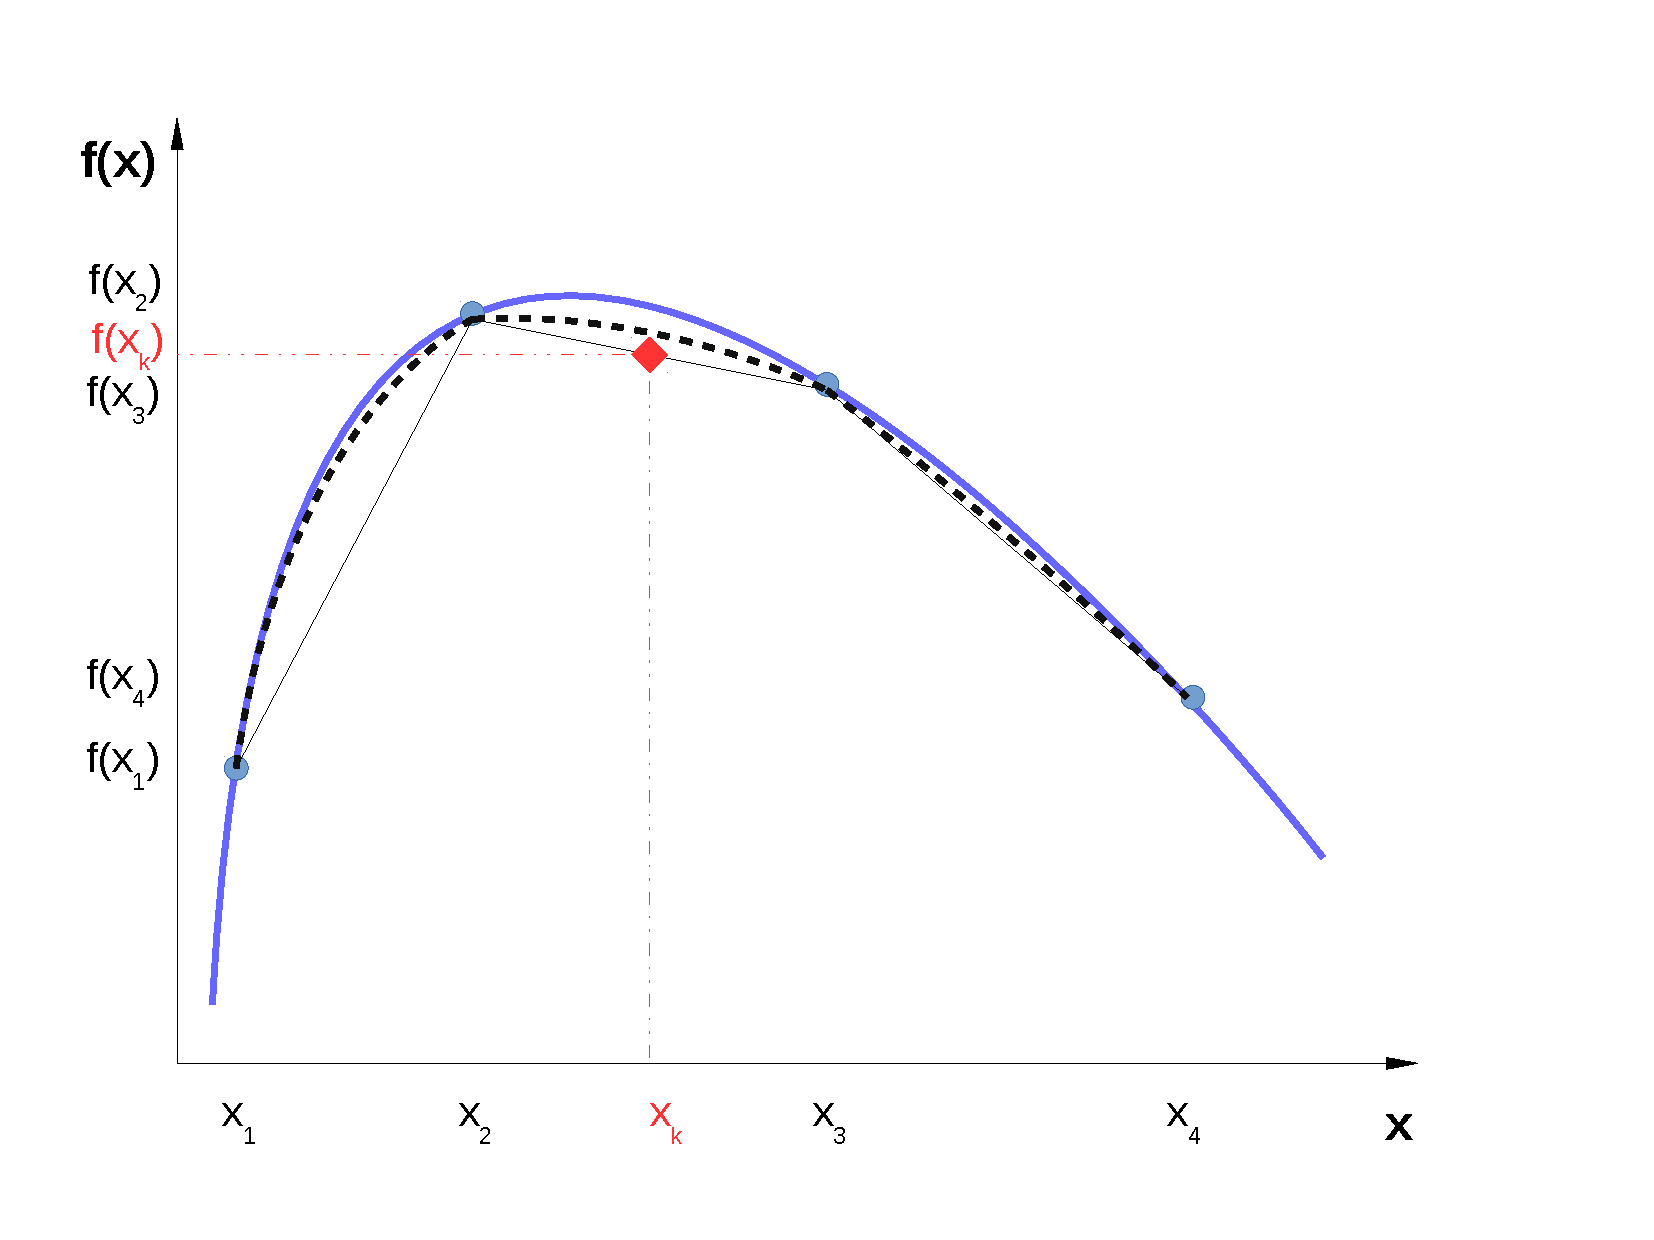
\includegraphics[width=\columnwidth,clip]{./../Pics/Interpolation}
           \caption{Smooth function $f(x)$ (solid blue line) may be more accurately interpolated by a high-order polynomial (black dotted line) than by a low-order polynomial (solid black line).} 
        \end{center}
      \end{figure}

    \begin{list}{\bf Example \arabic{qcounter}:~}{\usecounter{qcounter}}
%       
         \item Given a table of values for $f(x)=\tan{x}$ for a few values of $x$,
            \begin{center}
               \begin{tabular}{c | c c c c}
                   $x$        & 1.00   & 1.10   & 1.20   & 1.30   \\
                   \hline
                   $\tan{x}$  & 1.5574 & 1.9648 & 2.5722 & 3.6021 \\
               \end{tabular}
            \end{center}
            Estimate $\tan{1.15}$ and $\tan{1.23}$.

            {\bf Solution:} For $\left(x_{a}=1.10\right) < \left(x_{k}=1.15\right) < \left(x_{b}=1.20\right)$,
               \begin{eqnarray}
                  f\left(x_{k}\right) &=& \frc{f\left(x_{a}\right)\left(x_{b}-x_{k}\right) + f\left(x_{b}\right)\left(x_{k}-x_{a}\right)}{x_{b}-x_{a}} \nonumber \\
                                     &=& \frc{1.9648\times(1.20-1.15) + 2.5722\times(1.15-1.10)}{1.20-1.10} = 2.2685 \nonumber
               \end{eqnarray}

For  $\left(x_{a}=1.20\right) < \left(x_{k}=1.23\right) < \left(x_{b}=1.30\right)$,
               \begin{eqnarray}
                  f\left(x_{k}\right) &=& \frc{f\left(x_{a}\right)\left(x_{b}-x_{k}\right) + f\left(x_{b}\right)\left(x_{k}-x_{a}\right)}{x_{b}-x_{a}} \nonumber \\
                                     &=& \frc{2.5722\times(1.30-1.23) + 3.6021\times(1.23-1.20)}{1.30-1.20} = 2.8812 \nonumber
               \end{eqnarray}
%
         \item Calculate specific volume $\left(v, \text{in m}^{3}\text{.kg}^{-1}\right)$, internal energy $\left(u, \text{in kJ.kg}^{-1}\right)$ and entropy $\left(s, \text{in kJ.(kg.K)}^{-1}\right)$ of saturated water vapour at 133.45$^{\circ}$C.

           {\bf Solution:} From Appendix~\ref{Appendix:Saturated_SH_Tables} (Table A-2), for $T_{a}(=130.0) < T_{k} (= 133.45) < T_{b} (=140.0)^{\circ}C$, thus:
               \begin{eqnarray}
                  v\left(T_{k}\right) &=& \frc{v\left(T_{a}\right)\left(T_{b}-T_{k}\right) + v\left(T_{b}\right)\left(T_{k}-T_{a}\right)}{T_{b}-T_{a}} \nonumber \\
                                     &=& \frc{0.6685\times(140.0-133.45) + 0.5089\times(133.45-130.0)}{140.0-130.0} = 0.6134 \text{ m}^{3}\text{.kg}^{-1}\nonumber \\
                                     && \nonumber \\
                  u\left(T_{k}\right) &=& \frc{u\left(T_{a}\right)\left(T_{b}-T_{k}\right) + u\left(T_{b}\right)\left(T_{k}-T_{a}\right)}{T_{b}-T_{a}} \nonumber \\
                                     &=& \frc{2539.9\times(140.0-133.45) + 2550.0\times(133.45-130.0)}{140.0-130.0} = 2543.39 \text{ kJ.kg}^{-1}\nonumber \\
                                     && \nonumber \\
                  s\left(T_{k}\right) &=& \frc{s\left(T_{a}\right)\left(T_{b}-T_{k}\right) + s\left(T_{b}\right)\left(T_{k}-T_{a}\right)}{T_{b}-T_{a}} \nonumber \\
                                     &=& \frc{7.0269\times(140.0-133.45) + 6.9299\times(133.45-130.0)}{140.0-130.0} = 6.9934 \text{ kJ.}\left(\text{kg.K}\right)^{-1}\nonumber 
               \end{eqnarray}


    \end{list}

%%%
%%% SECTION
%%%
\section{Root-Finder Methods}\label{Section:RootFinderMethods}\index{Root-Finder Methods}

%%% SUBSECTION
\subsection{Motivation}
Given a smooth, {\it continuous} and {\it fully differentiable} function 
  \begin{displaymath}
     y = f(x) \hspace{3cm} \text{ with } x\in\mathbb{R}.
  \end{displaymath}
We aim to find the root $x=\psi$ of the function 
  \begin{displaymath}
     f(x) = 0.
  \end{displaymath}
The first step is to estimate $x_{0}$ that results in $f\left(x_{0}\right)\neq 0$ and may lead to a new estimate $x_{1}$. The procedure is repeated until $f\left(x_{n}\right)\rightarrow 0$ (\ie $x_{n}\approx\psi$), where $n$ is the number of repetitions (or {\it iterations}). There are several methods designed to solve non-linear equations, i.e., find the rrot of the function, here we will focus on the most popular {\it Newton-Raphson} method that combines simplicity and power.


%%% SUBSECTION
\subsection{Newton-Raphson Iterative Method}\label{Section:RootFinderMethods:NewtonRaphson}\index{Root-Finder Methods!Newton-Raphson method}
Let's assume that $x_{0}$ is a good estimate of the root$\psi$ and $\psi = x_{0} + h$. Since the root of the function $f(x)$ is $\psi$ and $h = \psi 0 x_{0}$, $h$ represents the distance between the initial estimate (or guess) and the root. Assuming $h$ is very (or {\it infinitesimal}) small, we can linearly approximate the function,
   \begin{displaymath}
        f\left(\psi\right) = 0 = f\left(x_{0}+h\right) \approx f\left(x_{0}\right) + h f'\left(x_{0}\right).
   \end{displaymath}
Therefore, except if $f'\left(x_{0}\right)$ is close to $0$, 
   \begin{displaymath}
        h \approx -\frc{f\left(x_{0}\right)}{f'\left(x_{0}\right)} \hspace{.3cm} \Longrightarrow \hspace{.3cm} \psi = x_{0} + h \approx x_{0} -\frc{f\left(x_{0}\right)}{f'\left(x_{0}\right)}.
   \end{displaymath}
%%% Figure
     \begin{figure}[h]\label{Appendix:Fig:NewtonRaphson}%
        \begin{center}
         \vbox{
           \hbox{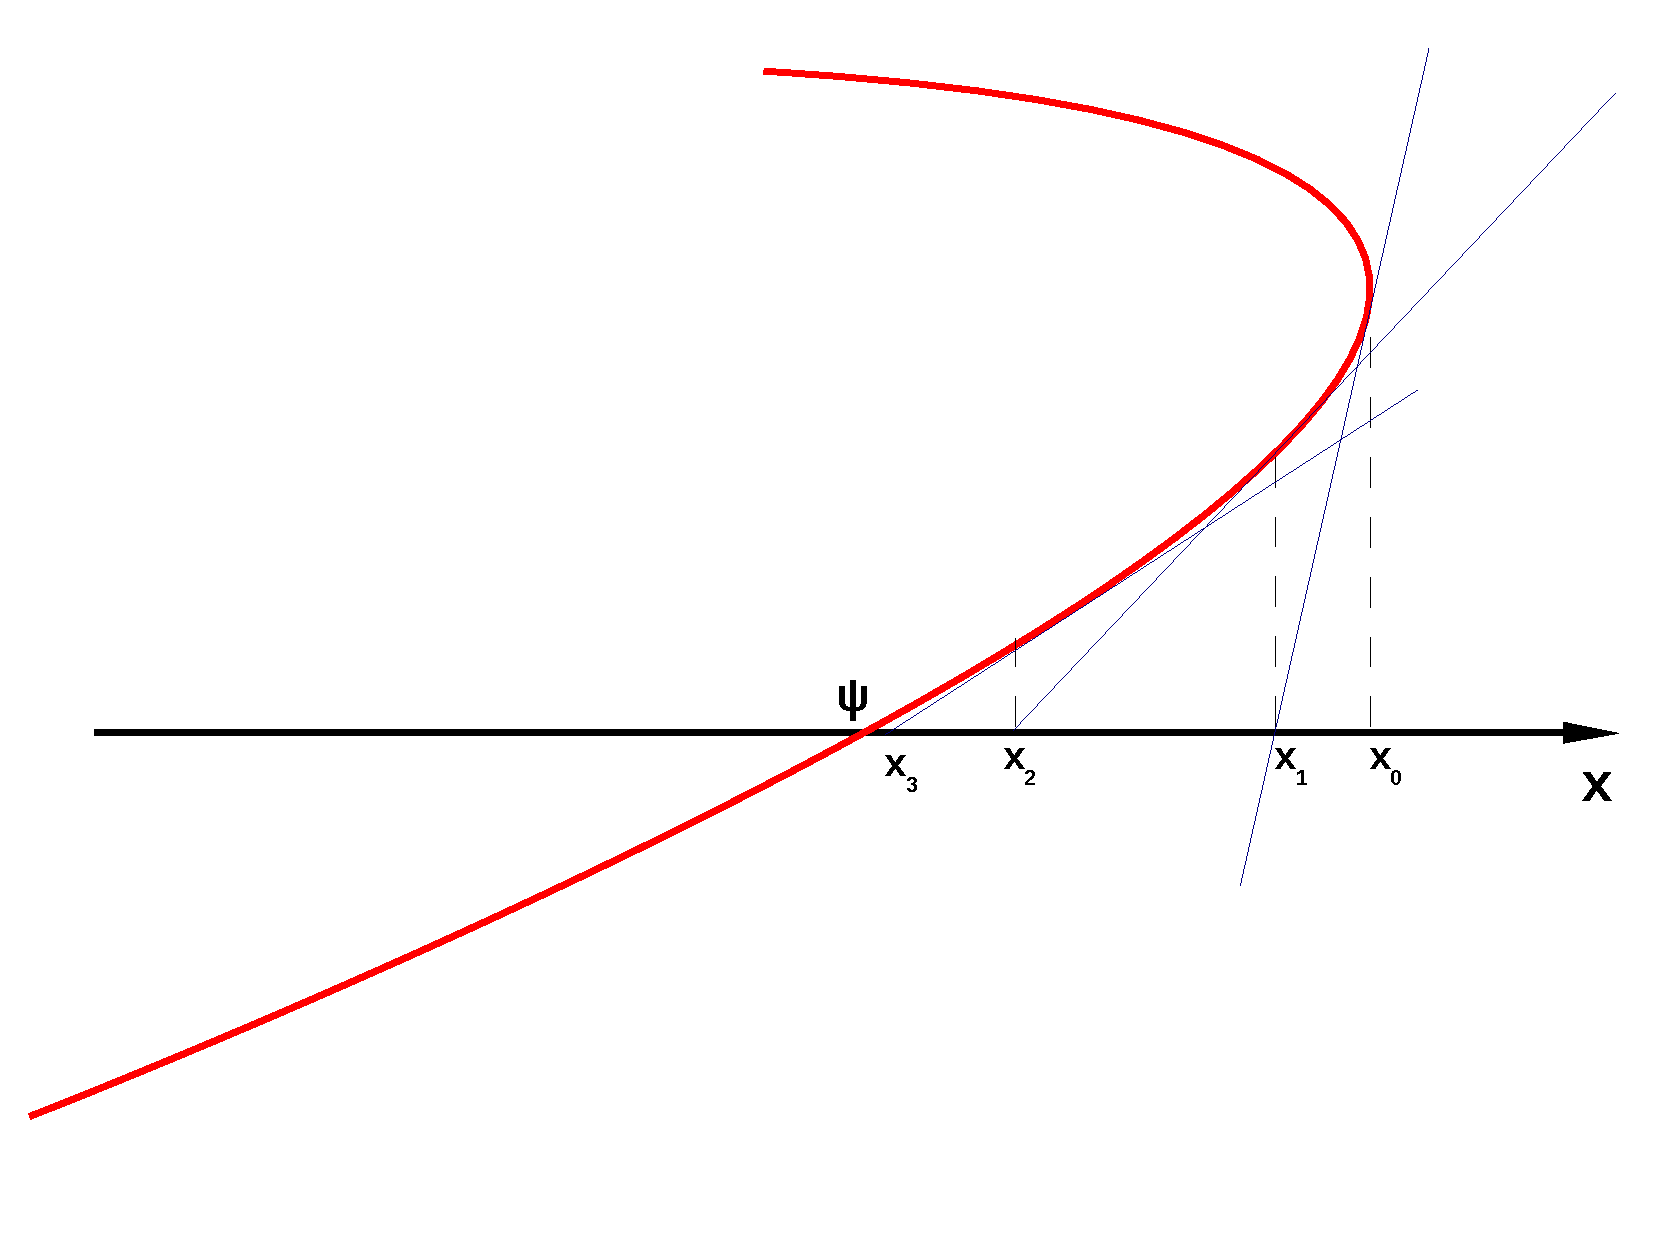
\includegraphics[width=\columnwidth,height=10cm]{./../Pics/NewtonRaphson2}}
           \hbox{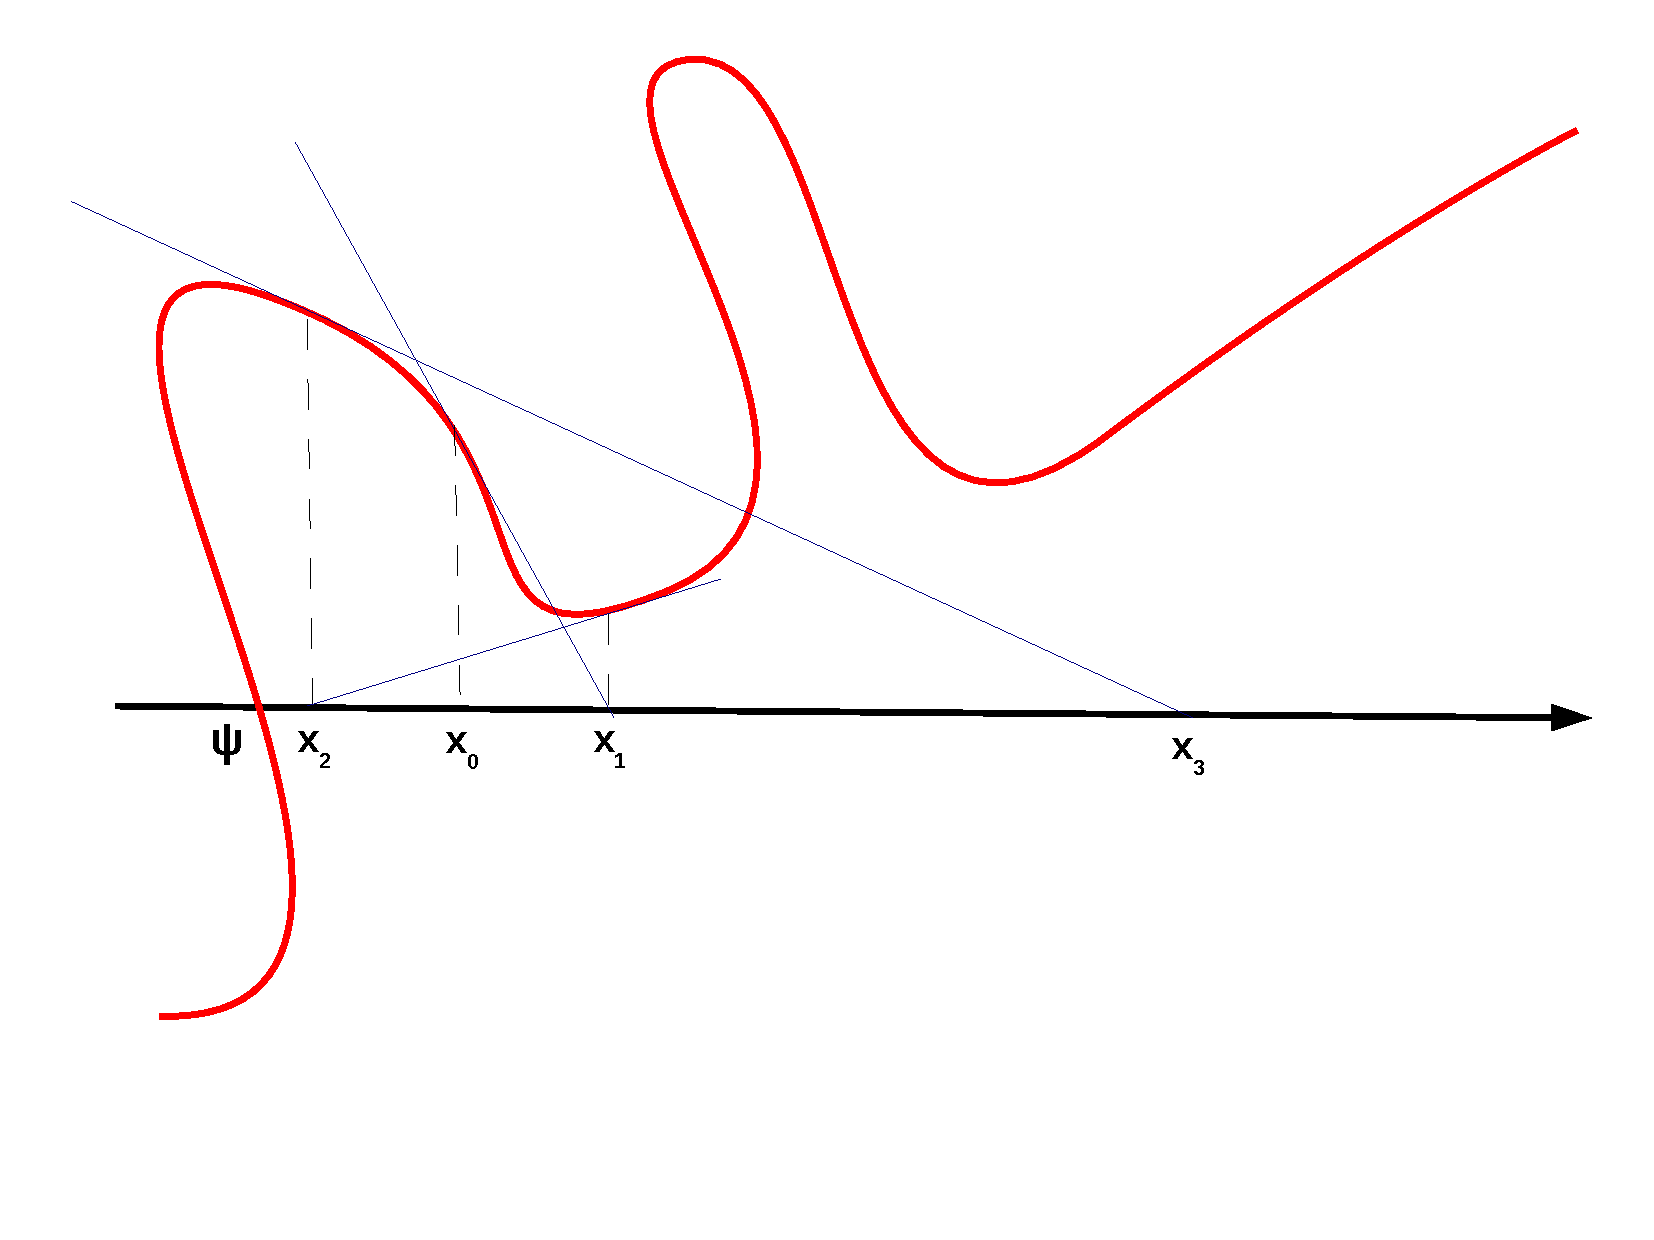
\includegraphics[width=\columnwidth,height=10cm]{./../Pics/NewtonRaphson3}}}
           \vspace{-1cm}
           \caption{Graphic representation of the Newton-Raphson iterative method: (top) solution of the smooth and continuous function $f(x)$ (solid red line) is approximated from the initial estimate $x_{0}$ to the final solution $x=\psi$; (bottom) initial estimate $x_{0}$ is far away from the root $\psi$ and the solution may diverge. Blue solid lines are tangent of the function at $x_{i}$.} 
        \end{center}
      \end{figure}
%
This expression represents an improvement of the original estimate, i.e.,  
   \begin{displaymath}
        x_{1} = x_{0} -\frc{f\left(x_{0}\right)}{f'\left(x_{0}\right)}.
   \end{displaymath}
The next estimate, $x_{2}$, is obtained from $x_{1}$, 
   \begin{displaymath}
        x_{2} = x_{1} -\frc{f\left(x_{1}\right)}{f'\left(x_{1}\right)}.
   \end{displaymath}

   \begin{shaded}
      We can generalise this expression for the $n-${\it th iteration},
         \begin{equation}
            x_{n+1} = x_{n} -\frc{f\left(x_{n}\right)}{f'\left(x_{n}\right)}.\label{NewtonRaphson:Eqn1}
         \end{equation}
   \end{shaded}

Figure~\ref{Appendix:Fig:NewtonRaphson}(a) shows a geometrical representation of the Newton-Raphson iterative method, where $m=f(x)$ is the tangent (blue) line at the coordinate pair $\left[x_{0},f\left(x_{0}\right)\right]$,
   \begin{displaymath}
     m = f\left(x_{0}\right) + \left(x-x_{0}\right)f'\left(x_{0}\right).
   \end{displaymath}
Let $x_{1}$ be the {\it x-intercept} of the tangent line, therefore
   \begin{displaymath}
     x_{1} = x_{0} - \frc{f\left(x_{0}\right)}{f'\left(x_{0}\right)}
   \end{displaymath}
The tangent line is a geometrical representation of the Newton-Raphson iterative method, Eqn.~\ref{NewtonRaphson:Eqn1}, as the estimates gradually tend to the root $\psi$ of the function. As it can be seen in the Fig.~\ref{Appendix:Fig:NewtonRaphson}(b), if the initial estimate $x_{0}$ is not close enough of the root $\psi$, the solution may not {\it converge}. In fact, the Newton-Raphson iterative method works most of the time if the initial estimate is {\it good enough}.

 From the {\it mean value theorem} (Theorem~\ref{Appendix:MeanValueTheorem}), let the function $f(x)$ be such that, 
   \begin{enumerate}[(a)]
      \item it is continuously differentiable in some open interval containing the solution $x=\psi$;
      \item $\left|f'(\psi)\right| < 1$.
   \end{enumerate}
Then there is a number $\epsilon > 0$ such that the iteration $x_{k+1}=f\left(x_{k}\right)$ {\it converges} whenever $x_{0}$ is chosen in $\left|x_{0}-\psi\right|\leq\epsilon$.

For bounded $x\in\mathbb{R}$ (\ie contained in the interval $a\leq x \leq b$), if $f''(x)$ exists and is continuous on $[a,b]$ and $\psi$ is a root of $f(x)$, that is, $f(\psi)=0$ and $f'(\psi)\neq0$. Thus for a function $g(x)$
    \begin{displaymath}
        g(x) = x - \frc{f(x)}{f'(x)}
    \end{displaymath}
with
    \begin{displaymath}
        g'(x) = 1 - \frc{[f'(x)]^{2} - f(x)f''(x)}{[f'(x)]^{2}} = \frc{f(x)f''(x)}{[f'(x)]^{2}},
    \end{displaymath}
and
    \begin{displaymath}
        g'(\psi) = \frc{f(\psi)f''(\psi)}{[f'(\psi)]^{2}}=0, \text{ since } f(\psi) = 0 \text{ and } f'(\psi) \neq 0
    \end{displaymath}
As $g'(x)$ is continuous, this means that there is a small neighbourhood around the root $x=\psi$ such that for all points $x$ in that neighbourhood, $\left|g'(x)\right|<1$.  Therefore, if $g(x)$ is chosen as above and the initial estimate $x_{0}$ is chosen {\it sufficiently close to the root} $x=\psi$, then the Newton-Raphson method is {\it guaranteed to converge}. 

Algorithm~\ref{Algorithm:NewtonRaphson} highlights the steps towards find the root of a function $f(x)$.

\begin{algorithm}[h]%\scriptsize
   \SetKwData{Left}{left}\SetKwData{This}{this}\SetKwData{Up}{up}
   \SetKwFunction{Union}{Union}\SetKwFunction{FindCompress}{FindCompress}
   \SetKwInOut{Input}{Input}\SetKwInOut{Output}{Output}\SetKwInOut{Calculate}{Calculate}\SetKwInOut{Set}{Set}\SetKwInOut{Adjust}{Adjust}\SetKwInOut{Assumption}{Assumption}

      \Input{Given the function $f(x)$, the initial estimate $x_{0}$, the error tolerance $\epsilon$ and the maximum number of iterations $N$:}
      \Output{An approximation to the root $x=\psi$}

      \Assumption{$x=\psi$ is a root of $f(x)$}

      \For{$k \leftarrow 0$ \KwTo $N$}{
             \Calculate{ $f\left(x_{k}\right)$ and $f'\left(x_{k}\right)$ }

             \Calculate{ $x_{k+1} = x_{k} - \frc{f\left(x_{k}\right)}{f'\left(x_{k}\right)}$ }

             \eIf{ $k == N$}{
                             {\it Calculation has \underline{not converged}. Modify the initial estimate $x_{0}$.} 
                   }{
                     \If{ $\left|f\left(x_{k}\right)\right| \leq \epsilon$ {\bf or} $\frc{\left|x_{k+1}-x_{k}\right|}{\left|x_{k}\right|} \leq \epsilon$ }{
                          {\it Stopping criteria} achieved. The root of function $f(x)$ is $\psi = x_{k+1}$
                          } }
          }
 \caption{Newton-Raphson method algorithm.}\label{Algorithm:NewtonRaphson}
\end{algorithm}

%%% SUBSECTION
\subsection{Secant Iterative Method}\label{Section:RootFinderMethods:Secant}\index{Root-Finder Methods!Secant method}
The Secant method is essentially the same as Newton-Raphson, however the derivative $f'(x)$ is approximated by a finite difference based on the current and the previous estimate for the root,
   \begin{displaymath}
       f'\left(x_{n}\right) \approx \frc{f\left(x_{n}\right) - f\left(x_{n-1}\right)}{x_{n}-x_{n-1}}
   \end{displaymath}

   \begin{shaded}
      Replacing the derivative in Eqn.~\ref{NewtonRaphson:Eqn1} for the $(n+1)^{\text{th}}$-{\it iteration},
         \begin{equation}
            x_{n+1} = x_{n} - \frc{ x_{n} - x_{n-1} }{f\left(x_{n}\right) - f\left(x_{n-1}\right)} f\left(x_{n}\right).\label{Secant:Eqn1}
         \end{equation}
   \end{shaded}
The main problem of the Secant iterative method is that it requires two initial estimates $x_{1}$ and $x_{0}$ for the calculations. These estimates must bound the solution, \ie, $x_{0} \leq \psi \leq x_{1}$. Algorithm~\ref{Algorithm:Secant} shows the steps for its implementation.


\begin{algorithm}[h]%\scriptsize
   \SetKwData{Left}{left}\SetKwData{This}{this}\SetKwData{Up}{up}
   \SetKwFunction{Union}{Union}\SetKwFunction{FindCompress}{FindCompress}
   \SetKwInOut{Input}{Input}\SetKwInOut{Output}{Output}\SetKwInOut{Calculate}{Calculate}\SetKwInOut{Set}{Set}\SetKwInOut{Adjust}{Adjust}\SetKwInOut{Assumption}{Assumption}

      \Input{Given the function $f(x)$, the initial estimates $x_{0}$ and $x_{1}$, the error tolerance $\epsilon$ and the maximum number of iterations $N$:}
      \Output{An approximation to the root $x=\psi$}

      \Assumption{$x=\psi$ is a root of $f(x)$}

      \For{$k \leftarrow 1$ \KwTo $N$}{
             \Calculate{ $f\left(x_{k}\right)$ and $f\left(x_{k-1}\right)$ }

             \Calculate{ $x_{k+1} = x_{k} - \frc{f\left(x_{k}\right)\left(x_{k}-x_{k-1}\right)}{f\left(x_{k}\right) - f\left(x_{k-1}\right)}$ }

             \eIf{ $k == N$}{
                             {\it Calculation has \underline{not converged}. Modify the initial estimate $x_{0}$.} 
                   }{
                     \If{ $\left|f\left(x_{k}\right)\right| \leq \epsilon$ {\bf or} $\frc{\left|x_{k+1}-x_{k}\right|}{\left|x_{k}\right|} \leq \epsilon$ }{
                          {\it Stopping criteria} achieved. The root of function $f(x)$ is $\psi = x_{k+1}$
                          } }
          }
 \caption{Secant method algorithm.}\label{Algorithm:Secant}
\end{algorithm}

\begin{list}{\bf Example \arabic{qcounter}:~}{\usecounter{qcounter}}
   \item\label{Example:Roots:Secant} Calculate the root of the function $f(x) = x^{2}-2$ using the Secant iterative method. The error tolerance is $\epsilon=10^{-5}$.
      \begin{description}
        \item[Solution:] The function
          \begin{displaymath}
               f(x) = x^{2} - 2, \text{ with initial estimates of } x_{0}=1.5 \text{ and } x_{1}=1.0.
          \end{displaymath}
          The Secant method is expressed through Eqn.~\ref{Secant:Eqn1} for the $(k+1)^{\text{th}}$-iteration,
          \begin{displaymath}
            x_{k+1} = x_{k} - \frc{ x_{k} - x_{k-1} }{f\left(x_{k}\right) - f\left(x_{k-1}\right)} f\left(x_{k}\right).
         \end{displaymath}
         \begin{list}{{\bf Iteration \arabic{mcounter}} (k=\arabic{mcounter}):~}{\usecounter{mcounter}}
            \item Calculating $x_{2}$ from $x_{0}$ and $x_{1}$:
                  \begin{eqnarray}
                      x_{2} &=& x_{1} - \frc{ x_{1} - x_{0} }{f\left(x_{1}\right) - f\left(x_{0}\right)} f\left(x_{1}\right) \nonumber \\
                           &=& 1 - \frc{1 - 1.5}{-1-0.25}  (-1) = 1.4
                  \end{eqnarray}
                  Stoppage criteria:
                    \begin{enumerate}[(a)]
                         \item $\left|f\left(x_{2}\right)\right| = 0.04 \leq \epsilon \hspace{2cm} \Longrightarrow$ \underline{False}
                         \item $\frc{\left|x_{2}-x_{1}\right|}{\left|x_{1}\right|} = 0.0667 \leq \epsilon \hspace{1.4cm} \Longrightarrow$ \underline{False}
                    \end{enumerate}
            \item Calculating $x_{3}$ from $x_{1}$ and $x_{2}$:
                  \begin{eqnarray}
                      x_{3} &=& x_{2} - \frc{ x_{2} - x_{1} }{f\left(x_{2}\right) - f\left(x_{1}\right)} f\left(x_{2}\right) \nonumber \\
                           &=& 1.4 - \frc{1.4 - 1.0}{-0.04-(-1)}  (-0.04) = 1.4167
                  \end{eqnarray}
                  Stoppage criteria:
                    \begin{enumerate}[(a)]
                         \item $\left|f\left(x_{3}\right)\right| = 0.0070 \leq \epsilon \hspace{2cm} \Longrightarrow$ \underline{False}
                         \item $\frc{\left|x_{3}-x_{2}\right|}{\left|x_{2}\right|} = 0.0193 \leq \epsilon \hspace{1.65cm} \Longrightarrow$ \underline{False}
                    \end{enumerate}
            \item Calculating $x_{4}$ from $x_{2}$ and $x_{3}$:
                  \begin{eqnarray}
                      x_{4} &=& x_{3} - \frc{ x_{3} - x_{2} }{f\left(x_{3}\right) - f\left(x_{2}\right)} f\left(x_{3}\right) \nonumber \\
                           &=& 1.4167 - \frc{1.4167 - 1.4}{0.0070-(-0.04)}  (0.0070) = 1.4142
                  \end{eqnarray}
                  Stoppage criteria:
                    \begin{enumerate}[(a)]
                         \item $\left|f\left(x_{4}\right)\right| = 3.84\times 10^{-5} \leq \epsilon \hspace{2cm} \Longrightarrow$ \underline{False}
                         \item $\frc{\left|x_{4}-x_{3}\right|}{\left|x_{3}\right|} = 1.76\times 10^{-3} \leq \epsilon \hspace{1.65cm} \Longrightarrow$ \underline{False}
                    \end{enumerate}
            \item Calculating $x_{5}$ from $x_{3}$ and $x_{4}$:
                  \begin{eqnarray}
                      x_{5} &=& x_{4} - \frc{ x_{4} - x_{3} }{f\left(x_{4}\right) - f\left(x_{3}\right)} f\left(x_{4}\right) \nonumber \\
                           &=& 1.4142 - \frc{1.4142 - 1.4167}{-3.84\times 10^{-5}-(0.0070)}  (-3.84\times 10^{-5}) = 1.4142
                  \end{eqnarray}
                  Stoppage criteria:
                    \begin{enumerate}[(a)]
                         \item $\left|f\left(x_{5}\right)\right| = 3.84\times 10^{-5} \leq \epsilon \hspace{2cm} \Longrightarrow$ \underline{False}
                         \item $\frc{\left|x_{5}-x_{4}\right|}{\left|x_{4}\right|} = 0.0 \leq \epsilon \hspace{3cm} \Longrightarrow$ \red{\underline{True}}
                    \end{enumerate}
         \end{list}
         Thus, \underline{4 iterations} were necessary to calculate the root of the function $f(x)=x^{2}-2$. The root of the function is \underline{$x=\psi=1.4142$}.
       \end{description}
         
%
   \item{Example:Roots:NewtonRaphson} Calculate the root of the same function of the previous example using the Newton-Raphson method.
      \begin{description}
        \item[Solution:] Now that we know the solution of the function, let's take the initial estimate as $x_{1}=1.5$. Newton-Raphson method is expressed through Eqn.~\ref{NewtonRaphson:Eqn1} for the $(k+1)^{\text{th}}$-iteration,
          \begin{displaymath}
            x_{k+1} = x_{k} - \frc{f\left(x_{k}\right)}{f'\left(x_{k}\right)}, \text{ where } f'\left(x_{k}\right) = 2x_{k}.
         \end{displaymath}
         \begin{list}{{\bf Iteration \arabic{qcounter}} (k=\arabic{qcounter}):~}{\usecounter{qcounter}}
            \item Calculating $x_{2}$ from $x_{1}$:
                  \begin{eqnarray}
                      x_{2} &=& x_{1} - \frc{f\left(x_{1}\right)}{f'\left(x_{1}\right)} = x_{1} - \frc{ x_{1}^{2}-2 }{ 2x_{1}}   \nonumber \\
                           &=& 1.5 - \frc{0.25}{3} = 1.4167
                  \end{eqnarray}
                  Stoppage criteria:
                    \begin{enumerate}[(a)]
                         \item $\left|f\left(x_{2}\right)\right| = 0.0070 \leq \epsilon \hspace{2cm} \Longrightarrow$ \underline{False}
                         \item $\frc{\left|x_{2}-x_{1}\right|}{\left|x_{1}\right|} = 0.0555 \leq \epsilon \hspace{1.4cm} \Longrightarrow$ \underline{False}
                    \end{enumerate}
            \item Calculating $x_{3}$ from $x_{2}$:
                  \begin{eqnarray}
                      x_{3} &=& x_{2} - \frc{f\left(x_{2}\right)}{f'\left(x_{2}\right)} = x_{2} - \frc{ x_{2}^{2}-2 }{ 2x_{2}}  \nonumber \\
                           &=& 1.4167 - \frc{0.0070}{2.8334} = 1.4142
                  \end{eqnarray}
                  Stoppage criteria:
                    \begin{enumerate}[(a)]
                         \item $\left|f\left(x_{3}\right)\right| = 3.84\times 10^{-5} \leq \epsilon \hspace{2cm} \Longrightarrow$ \underline{False}
                         \item $\frc{\left|x_{3}-x_{2}\right|}{\left|x_{2}\right|} = 1.77\times 10^{-3} \leq \epsilon \hspace{1.65cm} \Longrightarrow$ \underline{False}
                    \end{enumerate}
            \item Calculating $x_{4}$ from $x_{3}$:
                  \begin{eqnarray}
                      x_{4} &=& x_{3} - \frc{f\left(x_{3}\right)}{f'\left(x_{3}\right)} = x_{3} - \frc{ x_{3}^{2}-2 }{ 2x_{3}} \nonumber \\
                           &=& 1.4142 - \frc{-3.84\times 10^{-5}}{2.8284} = 1.4142
                  \end{eqnarray}
                  Stoppage criteria:
                    \begin{enumerate}[(a)]
                         \item $\left|f\left(x_{4}\right)\right| = 3.84\times 10^{-5} \leq \epsilon \hspace{2cm} \Longrightarrow$ \underline{False}
                         \item $\frc{\left|x_{4}-x_{3}\right|}{\left|x_{3}\right|} = 0 \leq \epsilon \hspace{3.3cm} \Longrightarrow$ \red{\underline{True}}
                    \end{enumerate}
         \end{list}
         Thus, we need \underline{3 iterations} to calculate the root, \underline{$x=\psi=1.4142$}, of the function. Now try to use $x_{1}=1.0$ as a first estimate and check how many iterations will be necessary to convergence.
       \end{description}
    You may have noticed that the function $f(x)=x^{2}-2$ has two real roots, $\sqrt{2}$ and $-\sqrt{2}$, and in the examples we only obtained the positive root. In order to find the negative root, we need to use initial estimates close enough to the solution, \eg $x_{0}=-1.5$·

\end{list}

     
\chapter{A Few Examples}

  \begin{list}{\bf Example \arabic{qcounter}:~}{\usecounter{qcounter}}
%
     %%% EXAMPLE 1:
     \item\label{example1} Using the cyclic rule (Appendix~\ref{Appendix_Calculus:Properties}) and the definitions,
    \begin{displaymath}
        \alpha = \frc{1}{V}\left(\frc{\partial V}{\partial T}\right)_{P} \hspace{1cm}\text{ and }\hspace{1cm} \beta = -\frc{1}{V}\left(\frc{\partial V}{\partial P}\right)_{T},
    \end{displaymath}
    \noindent show that 
    \begin{displaymath}
      \left(\frc{\partial P}{\partial T}\right)_{V} = \frc{\alpha}{\beta}.
    \end{displaymath}
%%
\medskip
     {\bf Solution:} From the cyclic rule,
       \begin{displaymath}
          \left(\frc{\partial P}{\partial T}\right)_{V}\left(\frc{\partial V}{\partial P}\right)_{T}\left(\frc{\partial T}{\partial V}\right)_{T} = -1.
       \end{displaymath}
     Thus,
       \begin{displaymath}
          \left(\frc{\partial P}{\partial T}\right)_{V} = \frc{-1}{\left(\frc{\partial V}{\partial P}\right)_{T}\left(\frc{\partial T}{\partial V}\right)_{T}} = \frc{-\left(\frc{\partial V}{\partial T}\right)_{P}}{\left(\frc{\partial V}{\partial P}\right)_{T}} = \frc{-V\alpha}{-V\beta} = \frc{\alpha}{\beta}
       \end{displaymath}
      
%
     %%% EXAMPLE 2:
     \item\label{example2} For a van der Waals gas, the pressure $P$ and the internal energy $U$ can be expressed as functions of the number of mols ($n$), total volume ($V$) and temperature ($T$),
       \begin{displaymath}
         P = \frc{n R T}{V-nb} - \frc{n^{2}a}{V^{2}} \hspace{1cm}\text{ and }\hspace{1cm} U = \frc{3}{2}n R T - \frc{n^{2}a}{V},
       \end{displaymath}
       respectively, where $a$ and $b$ are constants. Use these equations and the chain rule to derive an equation for $\left(\frc{\partial U}{\partial P}\right)_{n,T}$ in terms of $n$, $V$ and $T$.

%%
\medskip
{\bf Solution:}
   \begin{eqnarray}
      \Partial[U]{P}{n,T} &=& \Partial[U]{V}{n,T}\Partial[V]{P}{n,T} = \frc{\Partial[U]{V}{n,T}}{\Partial[P]{V}{n,T}} \nonumber \\
                          &=& \frc{\frc{n^{2}a}{V^{2}}}{\frc{2n^{2}a}{V^{3}}-\frc{n R T}{\left(V-nb\right)^{2}}} = \frc{n a}{\frc{2 n a}{V}-\frc{R T V^{2}}{\left(V-nb\right)^{2}}}\nonumber
   \end{eqnarray}
      
%
     %%% EXAMPLE 3:
     \item\label{example3} The heat capacity at constant volume is defined as $C_{v}\equiv \Partial[U]{T}{V}$. Show that
       \begin{displaymath}
          \Partial[U]{T}{P} = C_{v} + \alpha V\Partial[U]{V}{T},
       \end{displaymath}
       with $\alpha=\frc{1}{V}\Partial[V]{T}{P}$.

%
\medskip
       {\bf Solution:}
          \begin{displaymath}
            \Partial[U]{T}{P} = \Partial[U]{T}{V} + \Partial[U]{V}{T}\Partial[V]{T}{P},
          \end{displaymath}
          however $\Partial[U]{T}{V}=C_{v}$ and $\Partial[V]{T}{P}=V\alpha$. Thus,
          \begin{displaymath}
             \Partial[U]{T}{P} = C_{v} + \alpha V\Partial[U]{V}{T}.
          \end{displaymath}

%
     %%% EXAMPLE 4:
     \item\label{example4} h
%
\end{list}

  \end{appendix}

\cleardoublepage

\pagebreak

%\bibliographystyle{plain}
\bibliography{refbib}
\bibliographystyle{unsrt}

\cleardoublepage
\phantomsection
\renewcommand\leftmark{}
\renewcommand\rightmark{Index}
\addcontentsline{toc}{chapter}{Index}

\printindex


\end{document}
